\documentclass[12pt,a4paper]{article}

\usepackage[british,UKenglish]{babel}  %% Language
\usepackage[a4paper, margin=1in]{geometry} %% margins
\usepackage{cite}
\usepackage{natbib} %% References -- uncomment this if you want to use the Harvard referencing style
\usepackage{graphicx} %http://en.wikibooks.org/wiki/LaTeX/Importing_Graphics#Graphics_storage
\usepackage[export]{adjustbox}
\usepackage[absolute,overlay]{textpos}
\usepackage{tikz}
\usepackage{algorithm} % Code-Listings
\usepackage{algorithmic} % Code-Listings
\usepackage{subcaption}
% see http://www.ctan.org/tex-archive/macros/latex/contrib/algorithm2e/algorithm2e.pdf
% for more sophisticated algorithm listings
\usepackage{amsmath,amsfonts,amssymb}	% AMS mathematical facilities, fonts and symbols
\usepackage{lastpage}
\usepackage{datetime}
\usepackage[bookmarks=true, colorlinks=false]{hyperref}

\DeclareGraphicsExtensions{.pdf,.png,.jpg}
\graphicspath{{./figures/}} 

% Uncomment one of the following, according to your module name
% \newcommand{\mytype}{MSc Research Project / (Research) Practicum / Internship}
\newcommand{\mytype}{MSc Research Project}
%\newcommand{\mytype}{MSc (Research) Practicum}
%\newcommand{\mytype}{MSc Internship}

% Uncomment one of the following, according to your programme
\newcommand{\mystream}{Cloud Computing}


\newcommand{\myname}{Olumide Akinkunmi}
\newcommand{\studentID}{23351411}
\newcommand{\mytitle}{A Hyper-Heuristic Framework for Adaptive Task Scheduling in Heterogeneous Cloud Environments}

\newcommand{\supervisor}{Yasantha Samarawickrama}

\hypersetup{
 pdfauthor={\myname},
 pdftitle={\mytitle},
 pdfsubject={\mytype},
 pdfkeywords={\mystream}
}

\hyphenation{
% Man-age-ment
}

\includeonly{%
titlepage,
text/abstract,
text/introduction,
text/relatedwork,
text/implementation,
text/evaluation,
text/conclusion,
text/appendix
}

\begin{document}
%% titlepage.tex
%%

% coordinates for the bg shape on the titlepage
\providecommand{\diameter}{20}
\providecommand{\xone}{-15}
\providecommand{\xtwo}{160}
\providecommand{\yone}{15}
\providecommand{\ytwo}{-253}
\providecommand{\myinstitute}{School of Computing \\ National College of Ireland}

\begin{titlepage}
% bg shape
\begin{tikzpicture}[overlay]
\draw[color=gray]  
 		 (\xone mm, \yone mm)
  -- (\xtwo mm, \yone mm)
 arc (90:0:\diameter pt) 
  -- (\xtwo mm + \diameter pt , \ytwo mm) 
	-- (\xone mm + \diameter pt , \ytwo mm)
 arc (270:180:\diameter pt)
	-- (\xone mm, \yone mm);
\end{tikzpicture}
	\begin{textblock}{10}[0,0](7.75,1)
		
\includegraphics[width=.4\textwidth, center]{logos/NCI_Logos_RGB_NCI_Logo_Colour.png}
	\end{textblock}	
	\vspace*{3.5cm}
	\begin{center}
		\Huge{\mytitle}
		\vspace*{1cm}
		\large{Project Report}\\
		\vspace*{2cm}
		\Large{
			\mytype \\ \mystream
		}\\
		\vspace*{1cm}
		\huge{\myname}\\
			\Large{Student~ID:~\studentID}\\
		\vspace*{1cm}
		\Large{
			\myinstitute
		}
	\end{center}
	\vspace*{3cm}
\Large{
\begin{center}
\begin{tabular}[ht]{l c l}
 Supervisor: & \hfill  & \supervisor \\
\end{tabular}
\end{center}
}

\newdateformat{monthyear}{\monthname[\THEMONTH] \THEYEAR}
\begin{center}
\vspace*{1cm}
\large{\monthyear\today }
\end{center}


\begin{textblock}{10}[0,0](14,16.75)
\large{
	\textbf{www.ncirl.ie} 
}
\end{textblock}

\end{titlepage}

\title{\mytitle}%
\author{\myname \\ \studentID}%
\date{}
% \maketitle

\pagestyle{plain}
\pagenumbering{arabic}

\begin{abstract}
Heterogeneous cloud computing environments require efficient task scheduling to handle volatile workloads, cut operational costs, and reduce carbon footprints. Static heuristics like HEFT and Min-Min work well under specific conditions, but they fail when workload dynamics change or system faults occur. This dissertation presents a dynamic Multi-Armed Bandit (MAB) hyper-heuristic framework for cloud task scheduling. The architecture links a Python controller to a CloudSim Plus simulation backend using standard I/O streaming pipes. The controller manages a low-level heuristic pool of nine algorithms, including classical list schedulers, meta-heuristics, and local search methods. 

We evaluate four MAB selection mechanisms: $\epsilon$-Greedy, Standard UCB1, Discounted UCB, and Scaled Thompson Sampling. The framework uses a workload fingerprinting method based on the Coefficient of Variation ($\text{CoV}$) alongside a batch-relative multi-objective reward function balancing makespan, execution cost, carbon emissions, and resource utilization. We test the system using HPC2N and NASA real-world trace datasets. Experimental results show that Discounted UCB adapts best to non-stationary environments. When subjected to a 90\% capacity drop, Discounted UCB decayed legacy performance memory and shifted policy from meta-heuristics to PEFT within 10 rounds, whereas Standard UCB remained stuck in stale Q-values. Overall, the hyper-heuristic framework achieved up to a 34.3\% reduction in both operational costs and carbon emissions compared to traditional baselines.
\end{abstract}

%% introduction.tex
%%

%% ==============================
\section{Introduction}
\label{sec:Introduction}
\subsection{Background and Motivation}
As the demand for compute becomes larger than ever, data centers become a very critical part of modern digital infrastructure, because it gives organizations access to a scale of computational power which, in most cases, cannot be managed on-premises. To manage these physical machines means to efficiently assign arriving requests or tasks to Virtual Machines, while in accordance with SLA violations and maximizing hardware utilization. The problem now comes down to finding the best mode of allocation in a heterogeneous cloud environment.

With the emergence of AI/ML workloads, it becomes more important than ever to find a way to efficiently and consistently assign workloads to the right Virtual Machine Instance. These days, data centers are beginning to face heavier batch jobs that are also compute-heavy. Modern data center managers are also responsible for balancing trade-offs that aim to reduce makespan and financial costs, while also trying to maintain high hardware utilization \cite{Jeba2019Green}.

\subsection{Problem Statement}
Traditional scheduling algorithms such as Heterogeneous Earliest Finish Time, Min-Min and Max-Min have fixed rules that they follow, in terms of task metadata and resource availability; their strengths become their shortcomings in the context of a heterogeneous cloud environment. Meta-heuristic algorithms like Simulated Annealing use higher-level workflows to explore complex search spaces \cite{KUMAR20191}, but the problem comes from their high computational complexity which makes them unsuitable for high-velocity workloads.

As mentioned above, static or traditional scheduling algorithms cannot simply adapt to constantly changing workloads, and when this happens, resources are underutilized, SLAs are violated,  and operational costs balloon

\subsection{Proposed Solution}
This project presents a dynamic Multi-Armed Bandit (MAB) hyper-heuristic framework for task scheduling heterogeneous cloud environments. Instead of directly searching the task-to-VM space, it dynamically selects the low-level heuristic that provides the most optimal result from a pool of scheduling algorithms.

The framework consists of a Python decision plane and a Java CloudSim plus simulation application which communicate via Inter Process Communication(IPC). The framework uses a multi-objective reward function that tanh squashes multiple execution metrics into a single, readable score between 0 and 1.

\subsection{Key Contributions}
The main contributions of this dissertation are:
\begin{itemize}
    \item \textbf{Decoupled Hyper-Heuristic Architecture:} We build a lightweight, streaming Python-CloudSim Plus framework that selects low-level heuristics dynamically without interrupting execution streams.
    \item \textbf{Non-Stationary Adaptation under Failure:} We demonstrate that Discounted UCB outperforms standard bandit variants during abrupt system failures, pivoting its policy from computationally intensive meta-heuristics to PEFT within 10 rounds after a 90\% VM capacity loss.
    \item \textbf{Multi-Objective Carbon-Aware Reward Model:} We design a batch-relative reward function using a hyperbolic tangent ($\tanh$) transformation to balance makespan, financial cost, carbon emissions, and resource utilization without scale distortion.
    \item \textbf{Trace-Driven Empirical Validation:} We evaluate our framework using real-world HPC2N and NASA workload traces across 10-seed multi-seed runs.
\end{itemize}

\subsection{Report Structure}
The rest of this report is organized as follows: Section~\ref{sec:rw} reviews related literature on cloud task scheduling, multi-armed bandits, and sustainable hyper-heuristics. Section~\ref{sec:Methodology} provides the theoretical foundation for our MAB formulations and reward functions. Section~\ref{sec:Design} presents the system design and pipeline architecture. Section~\ref{sec:Implementation} details the software implementation and IPC integration. Section~\ref{sec:Evaluation} presents experimental results, sensitivity analyses, and statistical evaluations. Finally, Section~\ref{sec:Conclusion} concludes the report and discusses directions for future work.
\section{Related Work}
\label{sec:rw}

The landscape of task scheduling in data centers keeps evolving. It has moved from traditional prioritization towards much more intricate online learning frameworks. Traditional scheduling research was more focused on singular objectives like makespan, using algorithms like HEFT and PEFT \citep{HosseiniShirvani2021A}. These traditional algorithms are heavily reliant on the fact that the physical hardware is statically available; it does not factor in downtime into its scheduling process. This makes it suffer serious performance degradation when it experiences hardware faults. To help with these limitations, newer algorithms like Hybrid Swarm Optimizers were developed \citep{Alkaam2025Hybrid}.

The latest advancements in the space seem to have moved towards utilizing Deep Reinforcement Learning and Multi-Armed Bandit Algorithms \citep{Khan2025Machine,DeCarvalho2025Toward}. Using the Deep Reinforcement Learning methodology provides stellar results in stationary environments, but have very high training overhead \citep{Choppara2025Efficient,Sravan2026DRL}. Multi-Armed Bandit gives the option of using hyper-heuristics for lightweight online learning \citep{Singh2024Leveraging}

There are still three major gaps in the current literature:
\begin{enumerate}
    \item \textbf{Historical Bias in Non-Stationary Environments:} Standard MAB algorithms such as UCB and standard Thompson Sampling keep a very long performance history window, which makes it difficult for them to quickly react to unexpected capacity drops, or other hardware failures.
    \item \textbf{Lack of Lightweight Contextual Workload Fingerprinting:} Existing contextual or content-aware schedulers often rely on heavy offline classifiers or neural feature extractors \citep{Adil2022scp}. 
    \item \textbf{Unbalanced Multi-Objective Reward Formulations:} While sustainability and carbon intensity have emerged as first-class scheduling parameters alongside cost and latency \citep{Arora2023Towards}, existing multi-objective reward functions often suffer from scale distortion across heterogeneous execution batches, leading to single-metric dominance during bandit update steps.
\end{enumerate}

The remainder of this section critically reviews prior contributions across these foundational domains.

\subsection{Foundations of Non-Stationary Workload Allocation}
In heterogeneous cloud environments where tasks and requests don't all arrive in a sequential or predictable order, allocating resources becomes an NP-hard problem.

\citet{Mathew2014Study} categorised different scheduling algorithms around performance measures such as makespan, load balancing and throughput. \citet{Saurav2021A} takes this further by looking into energy-aware task scheduling in large, heterogeneous systems, and bargaining and exchange between execution speed and power consumption. All literature referenced in this section come to the same conclusion that traditional scheduling algorithms always underperform in heterogeneous environments.

\subsection{Deterministic Task Prioritization and Heuristic Approximations}
List-based algorithms like HEFT, PEFT and HSIP work in two stages: firstly, they rank the tasks, then they assign them to processors. This flow helps to make DAG scheduling less complex, and it provides predictable scheduling behaviour.

\citet{HosseiniShirvani2021A} uses this approach as a foundation to propose HH-LiSch: a hybrid list scheduler that combine two ranking strategies RankI and RankO. It was tested on benchmarks like Montage and Cybershake, and it saw a reduction in average makespan by 16.71\%, compared to HEFT and PEFT.

The major limitation is still the fact that classical list schedulers use fixed rules and limited workload information, and they do not learn from changing task characteristics.

\subsection{Content and Workload Feature Engineering for Scheduling}
Instead of treating each task as a singular unit of computation, using feature-informed schedulers use properties of the workload itself to examine task characteristics and determine resource allocation.

\citet{Adil2022scp} proposed CA-MLBS, a solution that combines both Support Vector Machine classification and Particle Swarm Optimization. The algorithm works by classifying incoming tasks by content type and maps them onto the most ideal machine available. Experiments showed that this method reduced makespan by up to 29\% and increased throughput by 44\% against feature-agnostic algorithms.

A major deterrent with this approach is that the classifier is trained offline, which means that once it is deployed, it does not adapt to changes in hardware or workload conditions.

\subsection{Complex Search Space Exploration in Hybrid Meta-Heuristics}

\citet{Kumar2021Implementation} applied Ant Colony Optimization (ACO) in CloudSim and reported lower average task execution times and cloudlet failure rates than Round Robin and Minimum Completion Time (MCT) policies.

Recent studies have gone further by combining several meta-heuristics, like \citet{Alkaam2025Hybrid}, who proposed HGHHC: which combines Henry Gas Solubility Optimization, Harris Hawks Optimization, and Comprehensive Opposition-Based Learning (COBL). Across HPC2N, NASA, and synthetic workload traces, HGHHC reduced makespan by 34.30\%, 72.95\%, and 28.67\% respectively, relative to the reported baseline swarm methods. \citet{Bal2022A} also proposed RATS-HM, which combines an improved cat swarm optimization scheduler (ICS-TS), a group optimization deep neural network (GO-DNN) and NSUPREME encryption for resource allocation and security.

The downside of this is that it is very computationally expensive, as these methods most likely require multiple population-based searched to properly assign tasks to resources. Having to repeatedly run this process for constantly changing workloads is expensive and may as well be too slow.

\subsection{Adaptive Online Decision-Making and Regret Minimization}

Multi-Armed Bandit models continuously learns from previous actions, rather than searching from scratch. The trade-off is between exploration and exploitation: where the algorithm tries lesser known actions, or it continues with actions that have previously performed well.

\citet{Singh2024Leveraging} proposed a MAB model for task scheduling that derives logarithmic regret bounds, as well as proposes latency and utilization improvements. \citet{Tran-Dang2024Parallel} merged Thompson Sampling with matching theory for a decentralised taks offloading through MAB-MATCH. \citet{Chigu2024A} developed an Upper Confidence Bound scheduler for serverless FaaS systems. Multi-Armed Bandits can also be used for federated learning under mobility constraints, as well as satellite beamforming \citep{Jun2025Mobility,Liang2026Joint}.

This approach stands out from the rest because of how highly adaptable it is. MAB-based algorithms can easily and confidently update their decisions as new information and performance feedback arrive. This is why they are a standout candidate for dynamic workloads.

A detailed taxonomy and feature comparison summarizing the literature alongside the characteristics of our proposed contextual MAB hyper-heuristic framework is presented in Table~\ref{tab:related_work_summary}.

\begin{table}[H]
\centering
\caption{Comprehensive Comparison of Literature and Features of the Proposed Work}
\label{tab:related_work_summary}
\small
\resizebox{\textwidth}{!}{%
\begin{tabular}{p{3.2cm} p{2.8cm} p{2.5cm} p{2.8cm} p{2.5cm} p{2.2cm} p{2.2cm}}
\toprule
\textbf{Study / Work} & \textbf{Methodology / Core Strategy} & \textbf{Optimization Objectives} & \textbf{Target Environment} & \textbf{Dynamic Adaptivity} & \textbf{Context / Feature Awareness} & \textbf{Evaluation Engine} \\
\midrule

\multicolumn{7}{l}{\textbf{\textit{List-Based \& Classical Heuristics}}} \\
\citet{HosseiniShirvani2021A} & HH-LiSch (Task duplication \& slot insertion) & Makespan & Cloud VMs & Static / Low & $\times$ & Simulation \\
\citet{Adil2022scp} & CA-MLBS (SVM + PSO content classification) & Makespan, Throughput & Cloud & Static & $\checkmark$ (Content Type) & CloudSim \\

\midrule
\multicolumn{7}{l}{\textbf{\textit{Meta-Heuristic \& Hybrid Approaches}}} \\
\citet{Kumar2021Implementation} & Ant Colony Optimization (ACO) & Execution Time, Failure Rate & Cloud & Moderate & $\times$ & CloudSim \\
\citet{Alkaam2025Hybrid} & HGHHC (Henry Gas + Harris Hawks + COBL) & Makespan & Heterogeneous Cloud & Moderate & $\times$ & HPC2N / NASA Traces \\
\citet{Bal2022A} & RATS-HM (Cat Swarm + GO-DNN + Encryption) & Utilization, Power, Security, Latency & Cloud / Edge & Moderate & $\times$ & CloudSim \\

\midrule
\multicolumn{7}{l}{\textbf{\textit{Machine Learning \& Neural Network Methods}}} \\
\citet{Daid2021An} & Probabilistic Neural Networks + Linear Regression & CPU Power, Allocation & Cloud Datacenters & High & $\checkmark$ (CPU Load) & MATLAB (10 VMs) \\
\citet{Sravan2026DRL} & Multi-Objective DRL Framework & Latency, Energy, SLA & Cloud / Fog & High & $\checkmark$ (SLA Bounds) & Simulation \\

\midrule
\multicolumn{7}{l}{\textbf{\textit{Multi-Armed Bandit (MAB) \& Hyper-Heuristic Schedulers}}} \\
\citet{Singh2024Leveraging} & Game-Theoretic MAB & Utilization, Latency, Fairness & Dynamic Cloud & High & $\times$ & Cloud Simulator \\
\citet{DeCarvalho2025Toward} & HHCSP (UCB-MAB + FRRMAB Credit Assignment) & Makespan, Cost, Carbon & Cloud (AWS / Teads) & High & $\times$ & Real AWS Data \\
\citet{Chigu2024A} & UCB-based MAB Scheduler & Execution Latency & Edge-Cloud FaaS & High & $\times$ & AWS Lambda / OpenWhisk \\



\midrule
\rowcolor{gray!15}
\textbf{Proposed Work} & \textbf{Contextual MAB Hyper-Heuristic (UCB / Discounted-UCB / Thompson) + IPC Bridge} & \textbf{Makespan, Utilization, Non-stationary Regret} & \textbf{Heterogeneous Edge-Cloud} & \textbf{High (Online Adaptive)} & \textbf{$\checkmark$ (Task Graph \& Workload Features)} & \textbf{CloudSim Plus (Java) + Python IPC Bridge} \\
\bottomrule
\end{tabular}%
}
\end{table}


%% methodology.tex
%%

%% ==============================
\section{Methodology}
\label{sec:Methodology}

% Building upon the gaps identified in Section~\ref{sec:rw}, this section expands on the theoretical and empirical methodology underpinning the framework. The problem space is formalized, the low-level heuristic pool is defined, the mathematical formulations for the MAB algorithms are presented, the workload fingerprinting and multi-objective reward model are explained, and the statistical evaluation protocol is outlined.

\subsection{Problem Formalization and System Model}
% Cloud task scheduling is modelled as a dynamic mapping problem where a stream of tasks $T = \{t_1, t_2, \dots, t_N\}$ arrives at an orchestration engine and must be mapped to a heterogeneous virtual machine pool $V = \{v_1, v_2, \dots, v_M\}$. Each VM $v_j$ is defined by its processing capacity $P_j$ (in Million Instructions Per Second, MIPS), operational cost rate $C_j$ (\$/s), and baseline power draw. Each task $t_i$ carries a length $L_i$ (in Million Instructions, MI) and memory requirement.

Task scheduling in the cloud is seen as a problem where tasks arrive at the data center and need to be assigned to a virtual machine. Each virtual machine has a processing capacity which is in Million Instructions per Second (MIPS), an operational cost rate and a baseline power draw. Each task has a size or length in Million Instructions, and a memory requirement.

The tasks are executed in batches. For each batch, a number of tasks arrives, and the scheduler selects a low level heuristic from a predefined pool of algorithms. The selected algorithm then determines the virtual machine each task is assigned to, which is then executed within CloudSim. Once the execution is complete, CloudSim returns netrics which the then transformed into a singular reward within the python program, to update the bandit's Q-values.

% Execution proceeds in batch decision rounds $k \in \{1, 2, \dots, K\}$. At round $k$, a workload batch $B_k \subset T$ arrives. The hyper-heuristic controller selects a Low-Level Heuristic (LLH) $a_k \in \mathcal{A}$ from a predefined pool of $K_{arms} = 9$ candidate algorithms. The selected arm $a_k$ generates a schedule mapping $B_k$ across $V$, which is then executed on the CloudSim Plus simulation backend. Upon completion, the backend returns batch execution metrics, which the hyper-heuristic transforms into a scalar reward $R_k \in [-1, 1]$ to update the bandit's internal Q-values.

\subsection{Low-Level Heuristic Pool}
The low-level heuristic pool consists of nine scheduling algorithms:
\begin{enumerate}
    \item \textbf{HEFT (Heterogeneous Earliest Finish Time):} Prioritizes tasks using upward rank values and assigning tasks to VMs with the earliest finish time.
    \item \textbf{PEFT (Predicting Earliest Finish Time):} Extends HEFT by incorporating an Optimistic Cost Table (OCT) to evaluate the downstream path impact.
    \item \textbf{Min-Min:} Assigns small tasks first to resources that execute them the fastest.
    \item \textbf{Max-Min:} Prioritizes large tasks first to prevent longer duration jobs from monopolizing compute resources toward the end of execution.
    \item \textbf{Round-Robin:} A deterministic baseline distributing tasks sequentially across active VMs regardless of task length or node capacity.
    \item \textbf{Sufferage:} Assigns tasks based on sufferage value (the difference between a task's second-earliest and earliest finish times), prioritizing tasks that face the greatest penalty if delayed.
    \item \textbf{HEFT with Duplication (HEFT-TD):} Duplicates critical predecessor tasks on redundant VM idle slots to eliminate inter-task communication latency.
    \item \textbf{Simulated Annealing (SA):} A probabilistic local search meta-heuristic that escapes local optima by accepting inferior schedule moves according to a decaying temperature schedule.
    \item \textbf{HGHHC:} A novel meta-heuristic integrating Henry Gas Solubility Optimization and Harris Hawks Optimization with Comprehensive Opposition-Based Learning \citep{Alkaam2025Hybrid}.
\end{enumerate}

\subsection{Multi-Armed Bandit Decision Algorithms}
We evaluate four MAB selection mechanisms to manage the exploration-exploitation trade-off under dynamic cloud conditions:

\subsubsection{$\epsilon$-Greedy}
Selects the arm with the highest estimated mean reward with probability $1 - \epsilon$, and explores a random arm with probability $\epsilon$ as shown in Equation~\eqref{eq:eqn_1}:
\begin{equation}
\label{eq:eqn_1}
a_k = \begin{cases} 
\arg\max_{a \in \mathcal{A}} \hat{Q}_k(a), & \text{with probability } 1 - \epsilon \\
\text{random arm } a \in \mathcal{A}, & \text{with probability } \epsilon 
\end{cases}
\end{equation}
where $\epsilon = 0.1$, and $\hat{Q}_k(a)$ is the empirical mean reward of arm $a$ up to round $k$.

\subsubsection{Standard UCB}
Constructs upper confidence bounds based on Hoeffding's Inequality to balance empirical performance and selection uncertainty shown in Equation~\eqref{eq:eqn_2}:
\begin{equation}
\label{eq:eqn_2}
a_k = \arg\max_{a \in \mathcal{A}} \left[ \hat{Q}_k(a) + c \cdot \sqrt{\frac{\ln k}{N_k(a)}} \right]
\end{equation}
where $N_k(a)$ is the total pull count of arm $a$ up to round $k$, and $c = \sqrt{2}$ is the exploration constant.

\subsubsection{Discounted UCB (D-UCB)}
Introduces a discount factor $\gamma \in (0, 1)$ to exponentially decay historical observations \citep{DeCarvalho2025Toward, Singh2024Leveraging} shown in Equations~\eqref{eq:eqn_3} and ~\eqref{eq:eqn_4}:
\begin{equation}
\label{eq:eqn_3}
\hat{Q}_k(\gamma, a) = \frac{\sum_{i=1}^{k-1} \gamma^{k-1-i} R_i \mathbb{I}(a_i = a)}{N_k(\gamma, a)}
\end{equation}
\begin{equation}
\label{eq:eqn_4}
N_k(\gamma, a) = \sum_{i=1}^{k-1} \gamma^{k-1-i} \mathbb{I}(a_i = a)
\end{equation}
The decision rule selects the arm maximizing the discounted upper bound shown in Equation~\eqref{eq:eqn_5}:
\begin{equation}
\label{eq:eqn_5}
a_k = \arg\max_{a \in \mathcal{A}} \left[ \hat{Q}_k(\gamma, a) + 2 B \sqrt{\frac{\xi \ln n_k(\gamma)}{N_k(\gamma, a)}} \right]
\end{equation}
where $n_k(\gamma) = \sum_{a \in \mathcal{A}} N_k(\gamma, a)$, $\gamma = 0.95$, $B = 1.0$ represents the reward bound, and $\xi = 0.5$ tunes exploration intensity.

\subsubsection{Scaled Thompson Sampling}
Maintains continuous probability distributions over expected rewards. At round $k$, sample values are drawn for each arm $a \in \mathcal{A}$, and the arm with the maximum sample is selected, shown in Equation~\eqref{eq:eqn_6}:
\begin{equation}
\label{eq:eqn_6}
a_k = \arg\max_{a \in \mathcal{A}} \theta_a
\end{equation}

% \subsection{Batch-Relative Multi-Objective Reward Function}
% To evaluate schedule quality without scale distortion across heterogeneous batches, raw metrics—Makespan ($M_k$, seconds), Monetary Cost ($C_k$, \$), Carbon Footprint ($E_k$, kg $\text{CO}_2\text{e}$), and Mean VM Utilization ($U_k \in [0, 1]$)—are converted into batch-relative performance ratios against a baseline schedule $a_{\text{base}}$ (Round-Robin), in Equation~\eqref{eq:eqn_10}:
% \begin{equation}
% \label{eq:eqn_10}
% \Delta M_k = \frac{M_k^{(a_{\text{base}})} - M_k^{(a_k)}}{M_k^{(a_{\text{base}})}}, \quad \Delta C_k = \frac{C_k^{(a_{\text{base}})} - C_k^{(a_k)}}{C_k^{(a_{\text{base}})}}, \quad \Delta E_k = \frac{E_k^{(a_{\text{base}})} - E_k^{(a_k)}}{E_k^{(a_{\text{base}})Sud}}
% \end{equation}
% The composite multi-objective metric combines efficiency gains and raw resource utilization, shown in Equation~\eqref{eq:eqn_11}:
% \begin{equation}
% \label{eq:eqn_11}
% S_k = w_1 \Delta M_k + w_2 \Delta C_k + w_3 \Delta E_k + w_4 U_k
% \end{equation}
% where weight vector $\boldsymbol{w} = [0.35, 0.25, 0.25, 0.15]$ satisfies $\sum w_i = 1.0$.

% To ensure stable gradient bounds for bandit updates, $S_k$ is passed through a hyperbolic tangent ($\tanh$) squashing function, mapping scalar performance into a bounded range $R_k \in [-1, 1]$, in Equation~\eqref{eq:eqn_12}:
% \begin{equation}
% \label{eq:eqn_12}
% R_k = \tanh\left( \lambda \cdot S_k \right)
% \end{equation}
% where $\lambda = 2.0$ acts as a steepness scaling factor.

\subsection{Evaluation Methodology}
To ensure rigorous empirical evaluation \citep{Zhao2025Scheduling}, our experimental methodology follows a structured pipeline:

\subsubsection{Trace Datasets}
We evaluate the system using two real-world high-performance computing workload traces from the Parallel Workloads Archive:
\begin{itemize}
    \item \textbf{HPC2N Trace:} Workload trace containing long execution profiles and heavy resource demands.
    \item \textbf{NASA Ames iPSC/860 Trace:} Shorter duration scale trace with dynamic arrival bursts and high arrival density.
\end{itemize}

\subsubsection{Non-Stationary Failure Injection}
To confirm how adaptable the scheduler is, we simulate an infrastructure failure event, where we reduce the available computing resources by 90\%.
%% design.tex
%%

%% ==============================
\section{Design Specification}
\label{sec:Design}
%% ==============================
This section outlines the architectural framework, functional requirements, component interactions, and algorithmic design underlying our dynamic Multi-Armed Bandit (MAB) hyper-heuristic system.

\subsection{System Requirements and Architectural Constraints}
To deliver adaptive, multi-objective scheduling without introducing runtime bottlenecks, the system architecture must meet five key technical requirements:
\begin{enumerate}
    \item \textbf{Decoupled Execution Architecture:} The decision engine and the cloud simulation environment must run in separate process spaces to allow modular updates to learning algorithms or simulation backends without cross-language bindings or tight coupling.
    \item \textbf{Low-Latency Inter-Process Communication (IPC):} Communication between the decision controller and the simulation platform must operate via high-throughput, streaming pipes to handle task arrival streams in real time.
    \item \textbf{Non-Stationary Adaptability:} The hyper-heuristic controller must continuously update internal policy states to recover quickly from sudden node drops or sudden shifts in workload volume.
    \item \textbf{Multi-Objective Metric Extraction:} The simulation backend must log fine-grained runtime metrics—makespan, execution cost, carbon emissions, and node-level VM utilization—at the end of every execution batch.
    \item \textbf{Trace-Driven Reproducibility:} The pipeline must support exact trace replay with controlled seed initialization to guarantee fair benchmarking across disparate bandit algorithms.
\end{enumerate}

\subsection{System Architecture and Streaming Pipe Pipeline}
The system uses a decoupled, event-driven architecture split into two main subsystems: a high-level \textbf{Python Hyper-Heuristic Decision Engine} and a \textbf{Java CloudSim Plus Simulation Backend}. Figure~\ref{fig:arch_pipeline} illustrates the structural design and streaming interface.

\begin{figure}[htbp]
\centering
\begin{verbatim}
+-----------------------------------------------------------------------+
|                 Python Hyper-Heuristic Decision Engine                |
|                                                                       |
|  +-----------------------+    +------------------------------------+  |
|  | Workload Fingerprinter |    | MAB Controller                     |  |
|  | (CoV Metrics Engine)  |    | (D-UCB / UCB1 / Thompson / eps-Gr) |  |
|  +-----------+-----------+    +-----------------+------------------+  |
|              |                                  |                     |
|              +-----------------+----------------+                     |
|                                | Action Selection (Arm ID)            |
+--------------------------------|--------------------------------------+
                                 |
                     JSON-Lines Pipe (Standard I/O)
                                 |
+--------------------------------|--------------------------------------+
|                                v                                      |
|  +-----------------------------------------------------------------+  |
|  | CloudSim Plus Java Simulation Backend                           |  |
|  |                                                                 |  |
|  |  +---------------------+       +-----------------------------+  |  |
|  |  | LLH Execution Pool  | ----> | Heterogeneous VM Pool       |  |  |
|  |  | (HEFT, PEFT, HGHHC) |       | (MIPS, Power, Carbon Model) |  |  |
|  |  +---------------------+       +-----------------------------+  |  |
|  +-----------------------------------------------------------------+  |
|                                |                                      |
|                    Batch Performance Feedback                         |
|                    (Makespan, Cost, Carbon, Util)                     |
+--------------------------------|--------------------------------------+
                                 |
                     JSON-Lines Pipe (Standard I/O)
                                 v
+-----------------------------------------------------------------------+
|                   Reward Transformer & State Updater                  |
|                   R_k = tanh( lambda * Composite_Score )              |
+-----------------------------------------------------------------------+
\end{verbatim}
\caption{System Architecture showing the Python Hyper-Heuristic Engine linked via Standard I/O streaming pipes to the CloudSim Plus backend.}
\label{fig:arch_pipeline}
\end{figure}

The interaction workflow proceeds as follows:
\begin{enumerate}
    \item \textbf{Batch Arrival and Workload Characterization:} The Python engine ingests a batch of tasks $B_k$ from the trace reader and calculates its Coefficient of Variation ($\text{CoV}_k$).
    \item \textbf{Action Selection:} The MAB controller passes $\text{CoV}_k$ to its selection rule ($\epsilon$-Greedy, UCB1, Discounted UCB, or Thompson Sampling) to pick an arm $a_k \in \mathcal{A}$.
    \item \textbf{Command Streaming:} The engine packages $a_k$ and $B_k$ metadata into a structured JSON-Lines payload and writes it to standard output.
    \item \textbf{Simulation Execution:} The Java CloudSim Plus process reads standard input, deserializes the JSON object, instantiates the chosen low-level heuristic, schedules the tasks across the active VM pool, and runs the simulation step.
    \item \textbf{Feedback Streaming:} Once the batch completes, CloudSim Plus calculates makespan, financial cost, carbon emissions, and VM utilization, serializes these metrics into JSON-Lines, and writes them back to standard output.
    \item \textbf{Reward Squashing and Policy Update:} The Python engine reads the feedback payload, computes the batch-relative reward $R_k \in [-1, 1]$ via the hyperbolic tangent function, and updates the bandit's Q-values or probability distributions.
\end{enumerate}

\subsection{Algorithmic Functionality of the Hyper-Heuristic Model}
Our core algorithm—the \textbf{Dynamic Workload-Aware Discounted MAB Hyper-Heuristic}, operates as a high-level policy wrapper over the pool of nine low-level heuristics. 

\subsubsection{Operational Logic}
Algorithm~\ref{alg:mab_hyper_heuristic} details the step-by-step decision framework running inside the Python orchestration controller.

\begin{algorithm}[H]
\caption{Dynamic Workload-Aware Discounted MAB Hyper-Heuristic}
\label{alg:mab_hyper_heuristic}
\begin{algorithmic}[1]
\REQUIRE Arm space $\mathcal{A} = \{1, \dots, 9\}$, discount factor $\gamma = 0.95$, exploration scale $c_0$, objective weights $\boldsymbol{w}$, total batches $K$.
\ENSURE Schedule mappings and updated bandit parameters.
\STATE Initialize $N(a) \leftarrow 0$, $\hat{Q}(a) \leftarrow 0$ for all $a \in \mathcal{A}$.
\FOR{each batch decision round $k = 1$ to $K$}
    \STATE Read arriving task batch $B_k$ from workload trace stream.
    \STATE Compute task length mean $\mu(B_k)$ and standard deviation $\sigma(B_k)$.
    \STATE Calculate trace volatility: $\text{CoV}_k \leftarrow \sigma(B_k) / \mu(B_k)$.
    \STATE Auto-tune exploration scale: $c_k \leftarrow c_0 \cdot (1 + \tanh(\text{CoV}_k - \text{CoV}_{\text{baseline}}))$.
    
    \IF{$k \le |\mathcal{A}|$}
        \STATE Select $a_k \leftarrow k$ \COMMENT{Warm-up phase: pull every arm once}
    \ELSE
        \FOR{each arm $a \in \mathcal{A}$}
            \STATE Compute discounted pull count: $N_k(\gamma, a) \leftarrow \sum_{i=1}^{k-1} \gamma^{k-1-i} \mathbb{I}(a_i = a)$.
            \STATE Compute discounted reward sum: $\hat{Q}_k(\gamma, a) \leftarrow \frac{\sum_{i=1}^{k-1} \gamma^{k-1-i} R_i \mathbb{I}(a_i = a)}{N_k(\gamma, a)}$.
        \ENDFOR
        \STATE Select arm: $a_k \leftarrow \arg\max_{a \in \mathcal{A}} \left[ \hat{Q}_k(\gamma, a) + 2 B \sqrt{\frac{\xi \ln \sum_b N_k(\gamma, b)}{N_k(\gamma, a)}} \right]$.
    \ENDIF
    
    \STATE Package $\{a_k, B_k\}$ into JSON payload and emit over standard I/O pipe.
    \STATE Read execution feedback $\{M_k, C_k, E_k, U_k\}$ from CloudSim Plus pipe.
    
    \STATE Compute relative efficiency metrics $\Delta M_k, \Delta C_k, \Delta E_k$ against Round-Robin baseline.
    \STATE Compute raw multi-objective score: $S_k \leftarrow w_1 \Delta M_k + w_2 \Delta C_k + w_3 \Delta E_k + w_4 U_k$.
    \STATE Squash reward: $R_k \leftarrow \tanh(\lambda \cdot S_k)$.
    
    \STATE Update Q-values and historical observation logs with decay factor $\gamma$.
\ENDFOR
\end{algorithmic}
\end{algorithm}

\subsubsection{Key Algorithmic Mechanisms}
\begin{itemize}
    \item \textbf{Dynamic Memory Decay:} By weighting past actions with $\gamma^{k-1-i}$, observations older than $1 / (1 - \gamma)$ rounds decay exponentially. When a capacity drop occurs at $k=50$, stale reward statistics from pre-failure rounds quickly lose influence, allowing the scheduler to drop previously dominant meta-heuristics in favor of fast, robust list schedulers like PEFT.
    \item \textbf{Scale-Invariant Multi-Objective Alignment:} Direct reward aggregation often causes the largest physical metric (e.g., makespan in seconds vs cost in cents) to dominate decisions. Normalizing performance relative to a Round-Robin baseline and squashing the output via $\tanh(\lambda \cdot S_k)$ keeps the reward signal stable within $[-1, 1]$, protecting the bandit from gradient explosion or scale distortion.
\end{itemize}

%% implementation.tex
%%

%% ==============================
\section{Implementation}
\label{sec:Implementation}
%% ==============================

This section describes the final implementation of the dynamic Multi-Armed Bandit (MAB) hyper-heuristic system. It covers the core software stack, inter-process orchestration pipeline, low-level heuristic pool, and structured data outputs.

\subsection{Technology Stack and Software Architecture}
The framework uses a two-tier software architecture built on two primary programming environments:
\begin{itemize}
    \item \textbf{Python Execution Engine (v3.11.7):} Serves as the primary control plane; housing the multi-armed bandit decision algorithms, workload trace ingestion module, statistical workload fingerprinter and reward transformer. It uses \texttt{NumPy} and \texttt{SciPy} for statistical operations and \texttt{Pandas} for trace parsing.
    \item \textbf{Java Simulation Engine (OpenJDK 21 / CloudSim Plus v7.3.0):} Acts as the cloud simulation environment. CloudSim Plus core classes were extended to support low-level heuristic instantiation and I/O streams
\end{itemize}

\subsection{Standard I/O Inter-Process Communication Pipeline}
In order to reduce the overhead of the spawning a new process for every CloudSim instance, we make use of inter-process communication to create a singular data stream between the Python control plane and the Java simulation engine.

The Python program launches the Java instance as a managed subprocess that receives a JSON payload containing the batch index and task specifications.

The Java application holds a stream reader that parses incoming JSON records asynchronously, which then executes the batch across the virtual machine pool.

\subsection{Low-Level Heuristic Pool Implementation}
The low-level heuristic pool is implemented inside the Java simulation core under a unified strategy interface, with nine distinct scheduling routines being implemented:
\begin{enumerate}
    \item \textbf{List-Based Schedulers (HEFT, PEFT, Min-Min, Max-Min, Sufferage, HEFT-TD):} Custom task prioritization routines construct directed acyclic graph (DAG) task ranks and evaluate expected finish times across heterogeneous VM capacity matrices on the fly.
    \item \textbf{Deterministic Baseline (Round-Robin):} Sequentially maps incoming cloudlets to active VMs to establish a dynamic baseline for performance normalization.
    \item \textbf{Local Search and Meta-Heuristics (Simulated Annealing, HGHHC):} Algorithmic state models execute local schedule permutations. HGHHC integrates Henry Gas Solubility Optimization and Harris Hawks Optimization search mechanics, running iterative candidate schedule evaluations within bounded CloudSim time slots.
\end{enumerate}

\subsection{Energy, Carbon Footprint, and Cost Modeling}
To evaluate multi-objective trade-offs accurately, custom tracking modules were integrated directly into the CloudSim Plus Datacenter engine:
\begin{itemize}
    \item \textbf{Monetary Cost Model:} This models dynamic cloud resource pricing, with the help of AWS billing API. Each VM instance incurs a fixed per-second compute rate based on its allocated processing capacity (MIPS) and memory profile, following tier-based provider pricing schemes.
    \item \textbf{Dynamic Power Model:} Power consumption $P(u)$ is calculated as a function of instantaneous CPU utilization $u \in [0, 1]$:
    \begin{equation}
    P(u) = P_{\text{idle}} + (P_{\text{max}} - P_{\text{idle}}) \times u
    \end{equation}
    where $P_{\text{idle}}$ represents baseline VM standby power, and $P_{\text{max}}$ denotes peak power under full load.
\end{itemize}

\subsection{Non-Stationary Infrastructure Fault Injection}
An automated fault injection module was implemented in the Python environment to simulate physical infrastructure failure. The purpose of this is to monitor and evaluate how each bandit algorithm reacts to an instantaneous change in physical environments. The module shuts down seven of the eight provisioned virtual machines, thereby forcing all incoming tasks to a single machine.

\subsection{Generated Outputs and Data Transformation}
The execution pipeline produces artefacts for post-hoc analysis:
\begin{enumerate}
    \item \textbf{Raw Trace Log Stream:} JSON files generated per run that hold batch-level decision metrics such as selected heuristic arm, raw makespan, monetary cost, carbon output, VM utilization, and squashed reward $R_k$.
    \item \textbf{Aggregated Seed Benchmark Dataset:} Structured CSV files combining metrics across all 10 random seeds per MAB variant and trace dataset.
\end{enumerate}

\section{Evaluation}
\label{sec:Evaluation}

This section presents a comprehensive empirical evaluation of our dynamic Multi-Armed Bandit (MAB) hyper-heuristic framework evaluated against real-world HPC workload traces from HPC2N and NASA Ames iPSC/860. We examine policy evolution dynamics, cumulative makespan trajectories, multi-objective trade-off profiles, and cross-algorithm selection heatmaps.

\subsection{Experimental Results and Comparative Analysis}

\subsubsection{Heuristic Selection Ratio Evolution}
Figures~\ref{fig:selection_evolution_hpc2n} and~\ref{fig:selection_evolution_nasa} track the temporal evolution of low-level heuristic (LLH) selection ratios across 100 simulation rounds using a 10-round moving window.

\begin{figure}[htbp]
    \centering
    \begin{subfigure}[b]{0.48\textwidth}
        \centering
        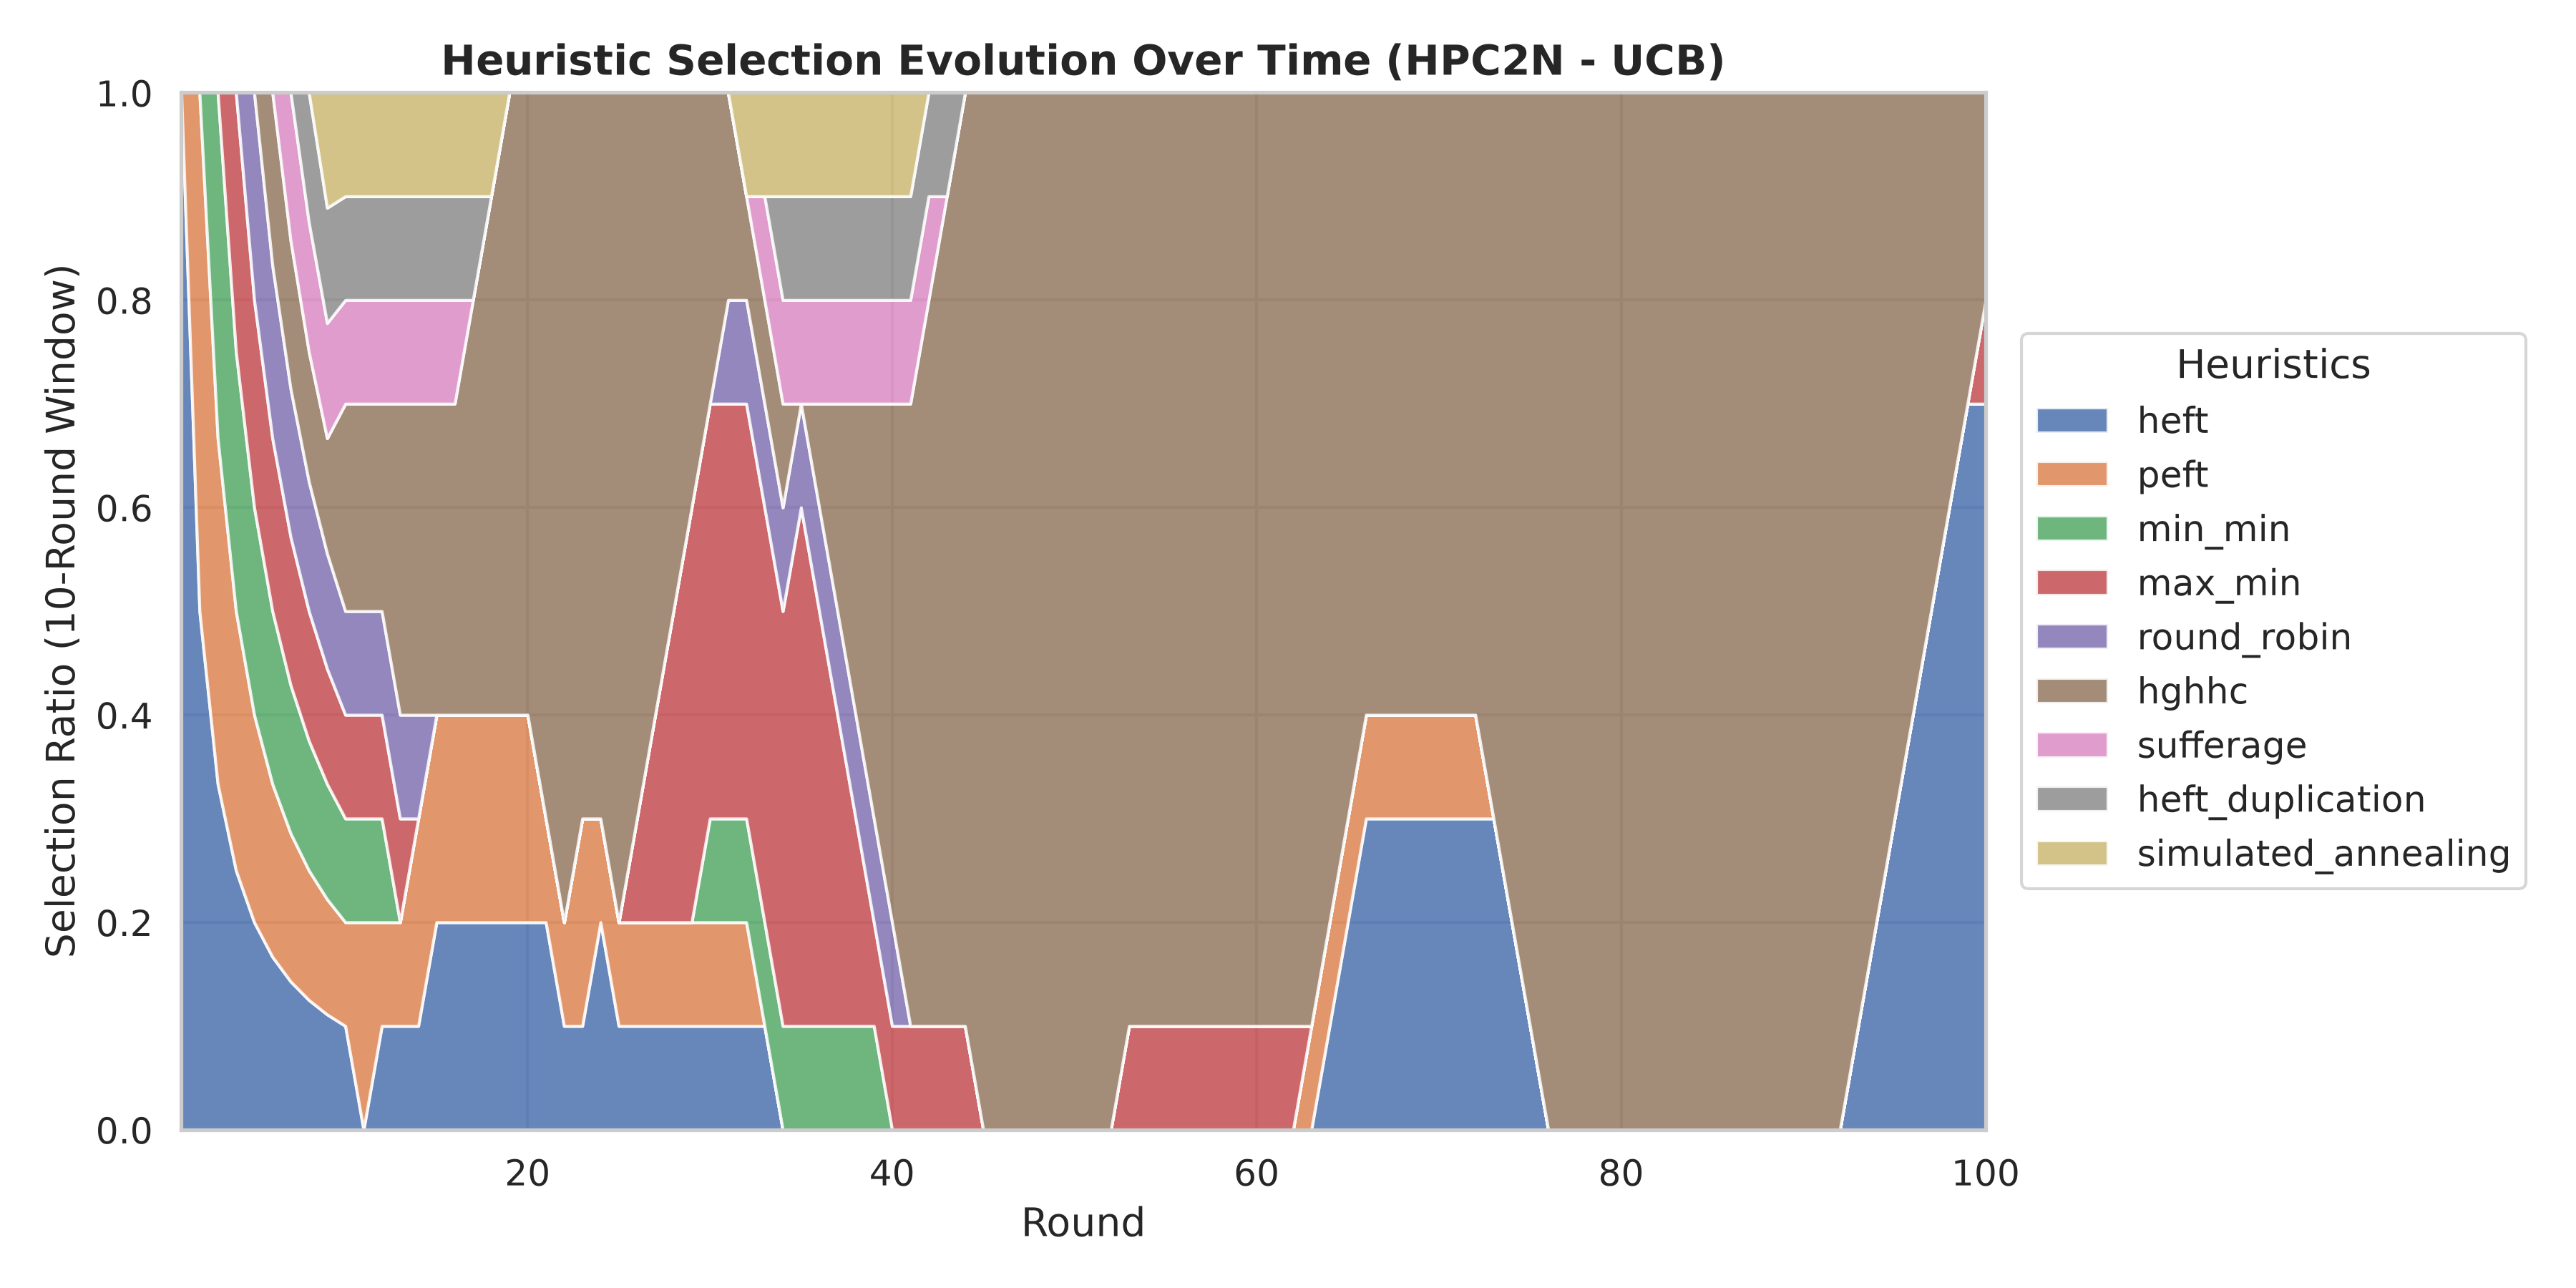
\includegraphics[width=\textwidth]{hpc2n_ucb_arm_selection_evolution.png}
        \caption{HPC2N -- UCB}
        \label{fig:selection_hpc2n_ucb}
    \end{subfigure}
    \hfill
    \begin{subfigure}[b]{0.48\textwidth}
        \centering
        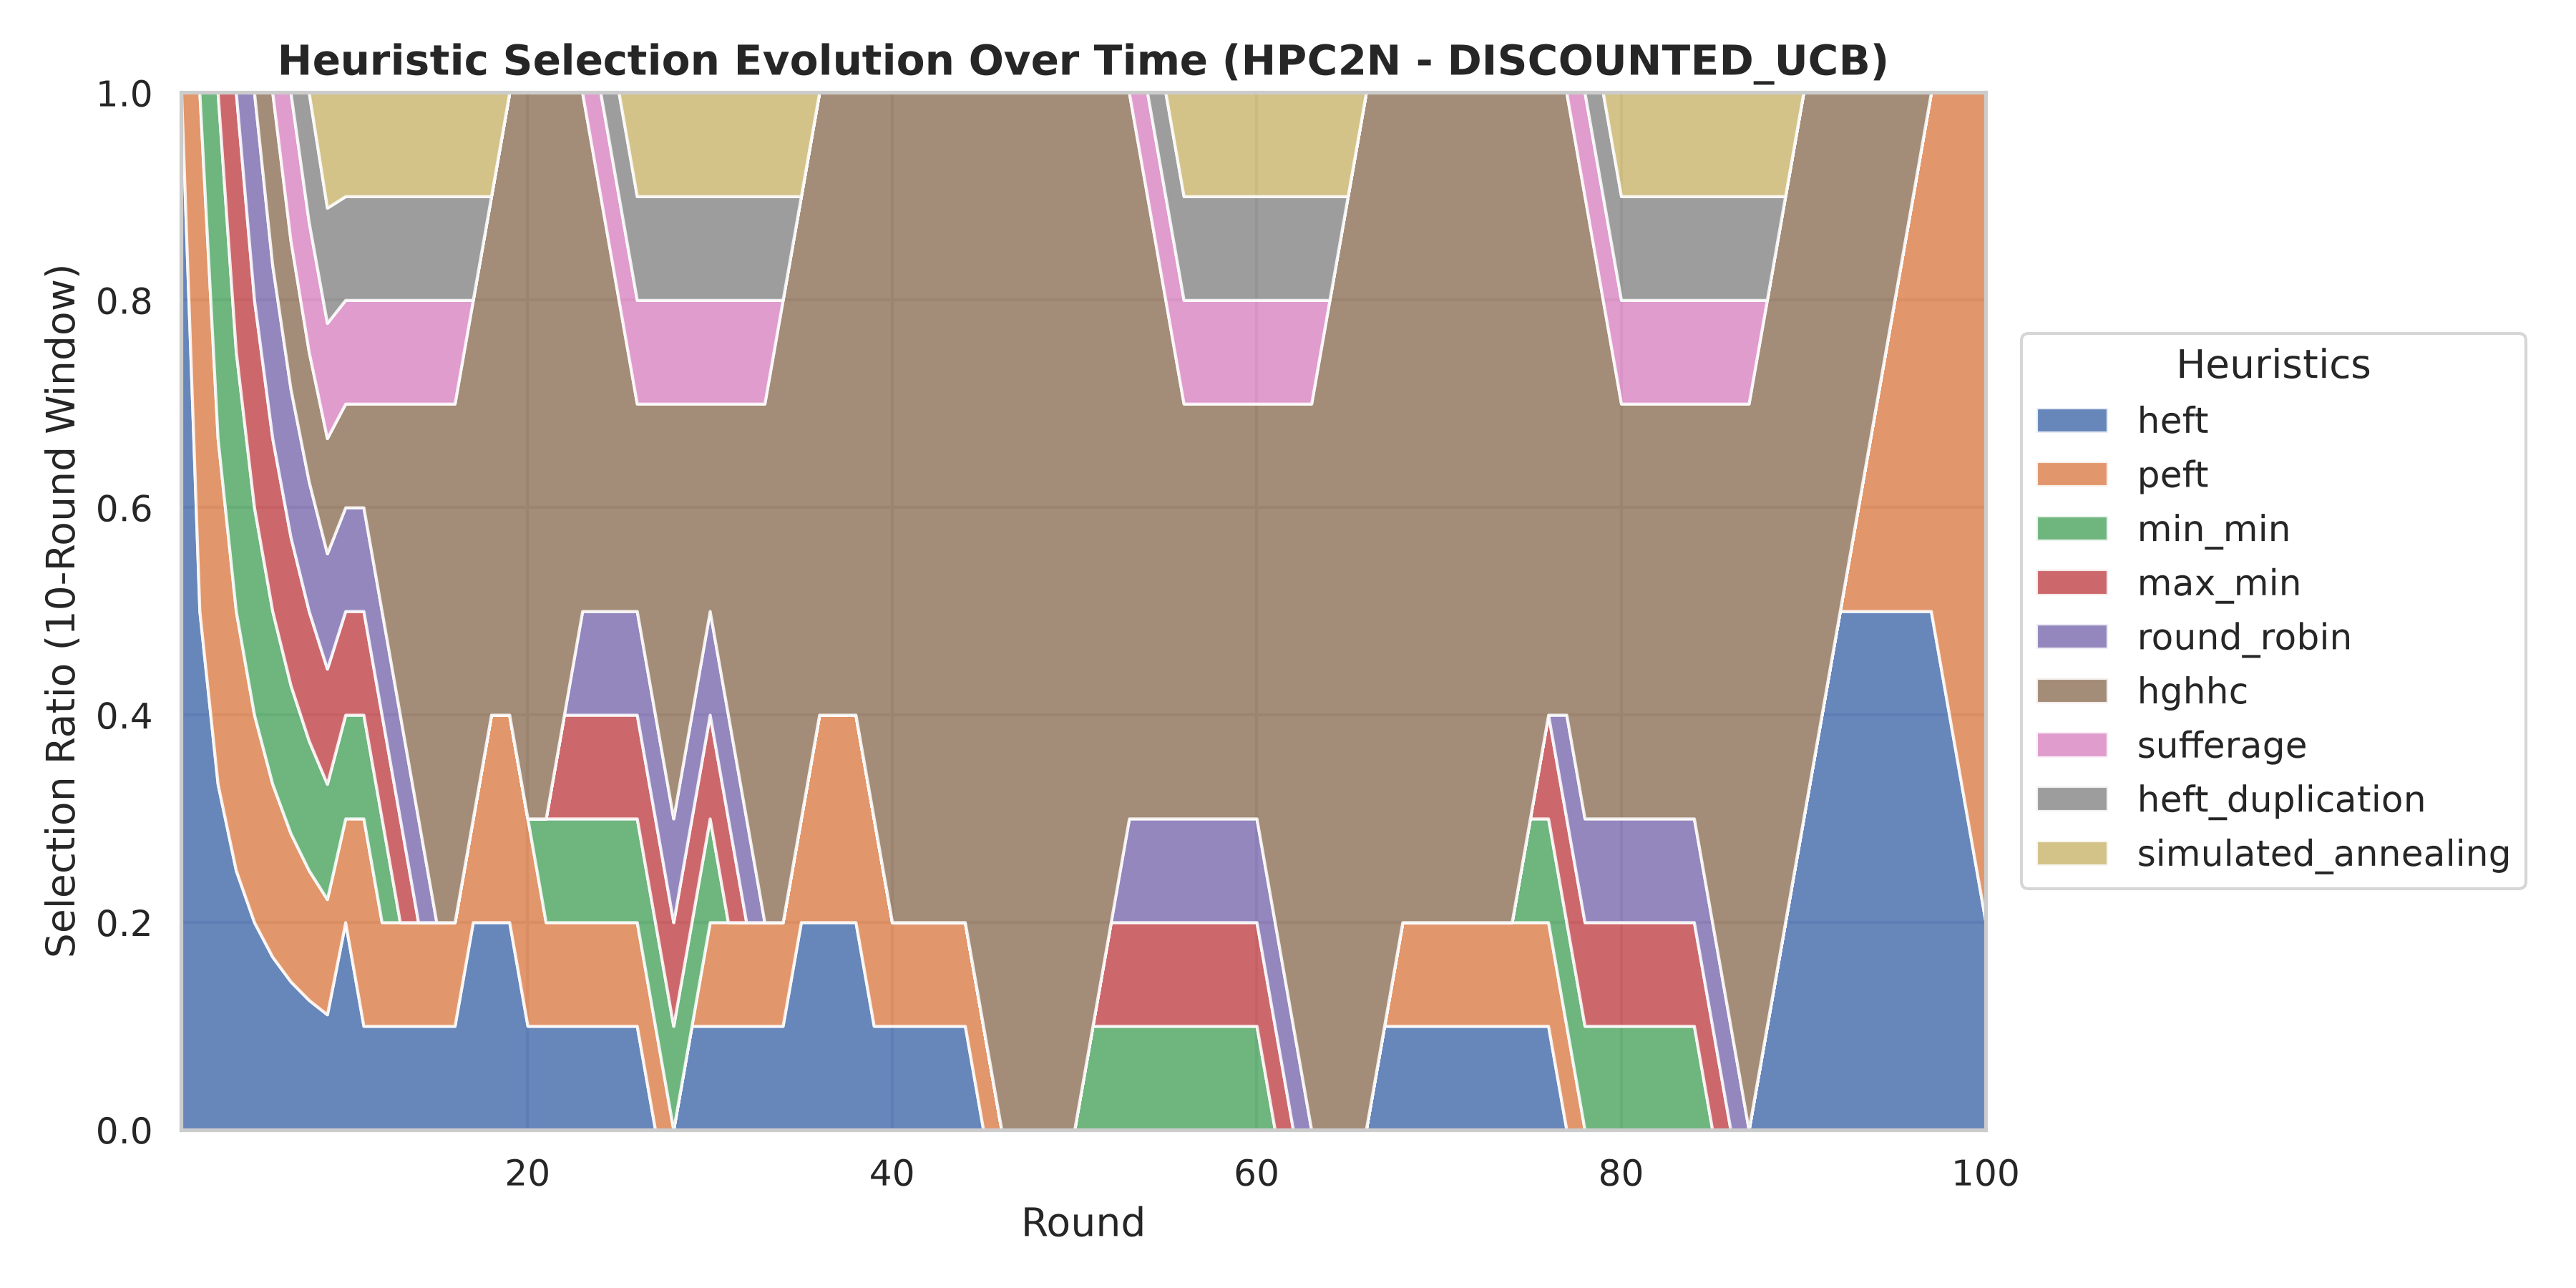
\includegraphics[width=\textwidth]{hpc2n_discounted_ucb_arm_selection_evolution.png}
        \caption{HPC2N -- Discounted UCB}
        \label{fig:selection_hpc2n_discounted}
    \end{subfigure}
    \vskip\baselineskip
    \begin{subfigure}[b]{0.48\textwidth}
        \centering
        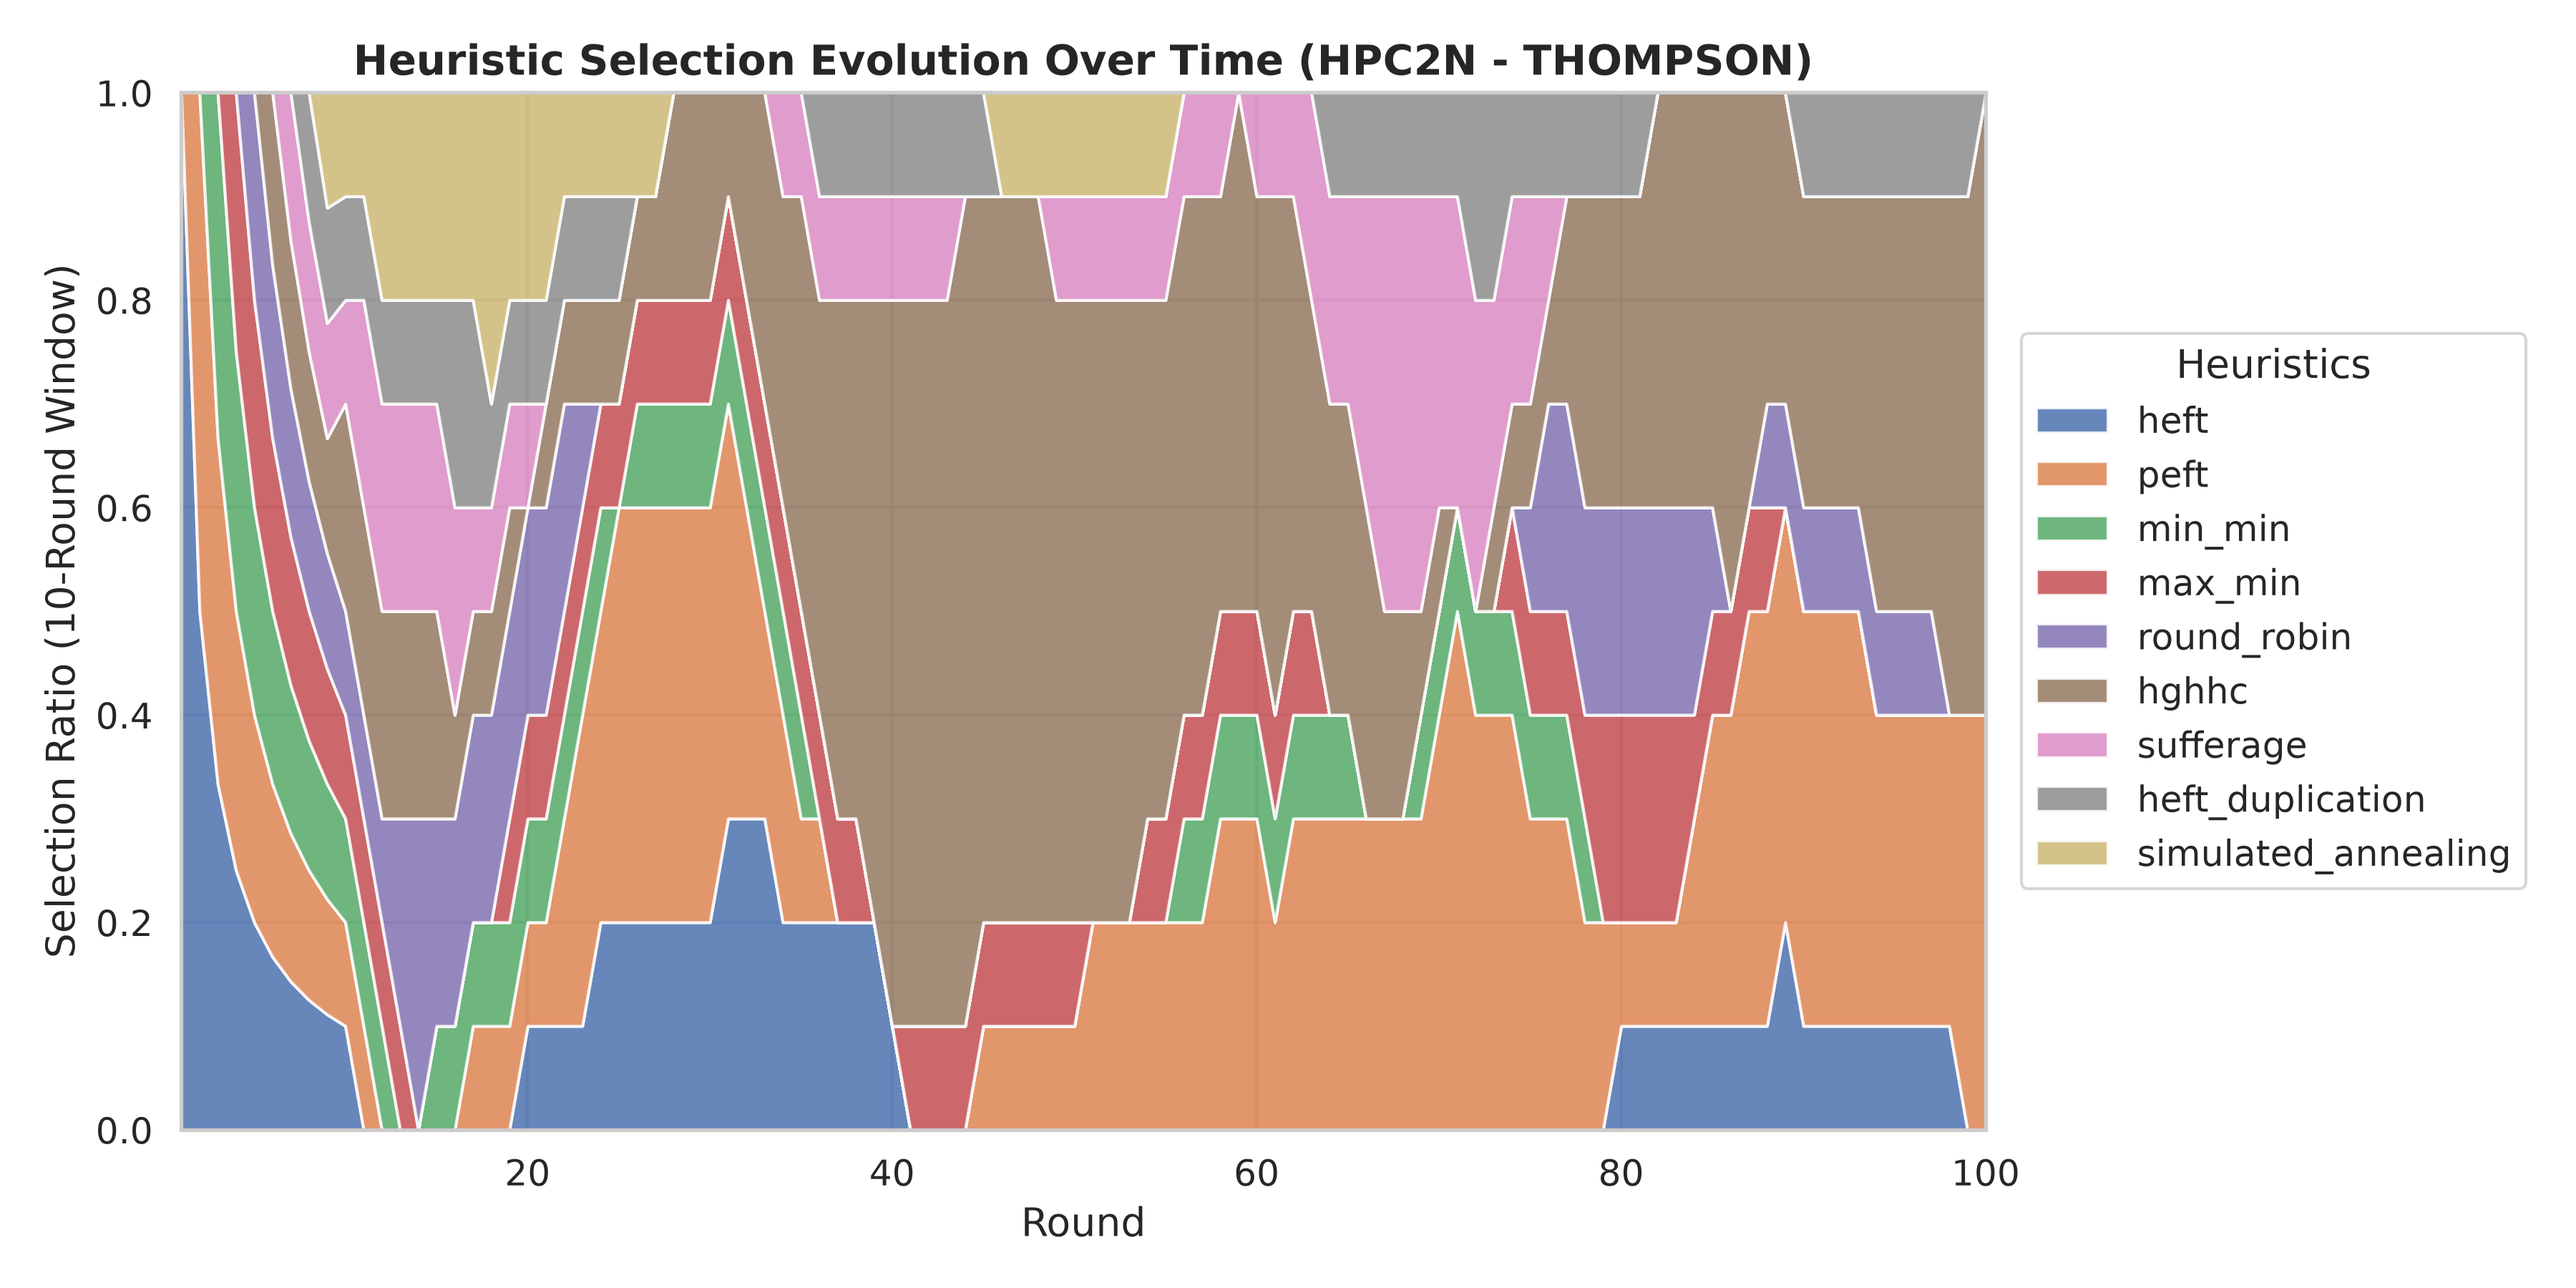
\includegraphics[width=\textwidth]{hpc2n_thompson_arm_selection_evolution.png}
        \caption{HPC2N -- Thompson Sampling}
        \label{fig:selection_hpc2n_thompson}
    \end{subfigure}
    \hfill
    \begin{subfigure}[b]{0.48\textwidth}
        \centering
        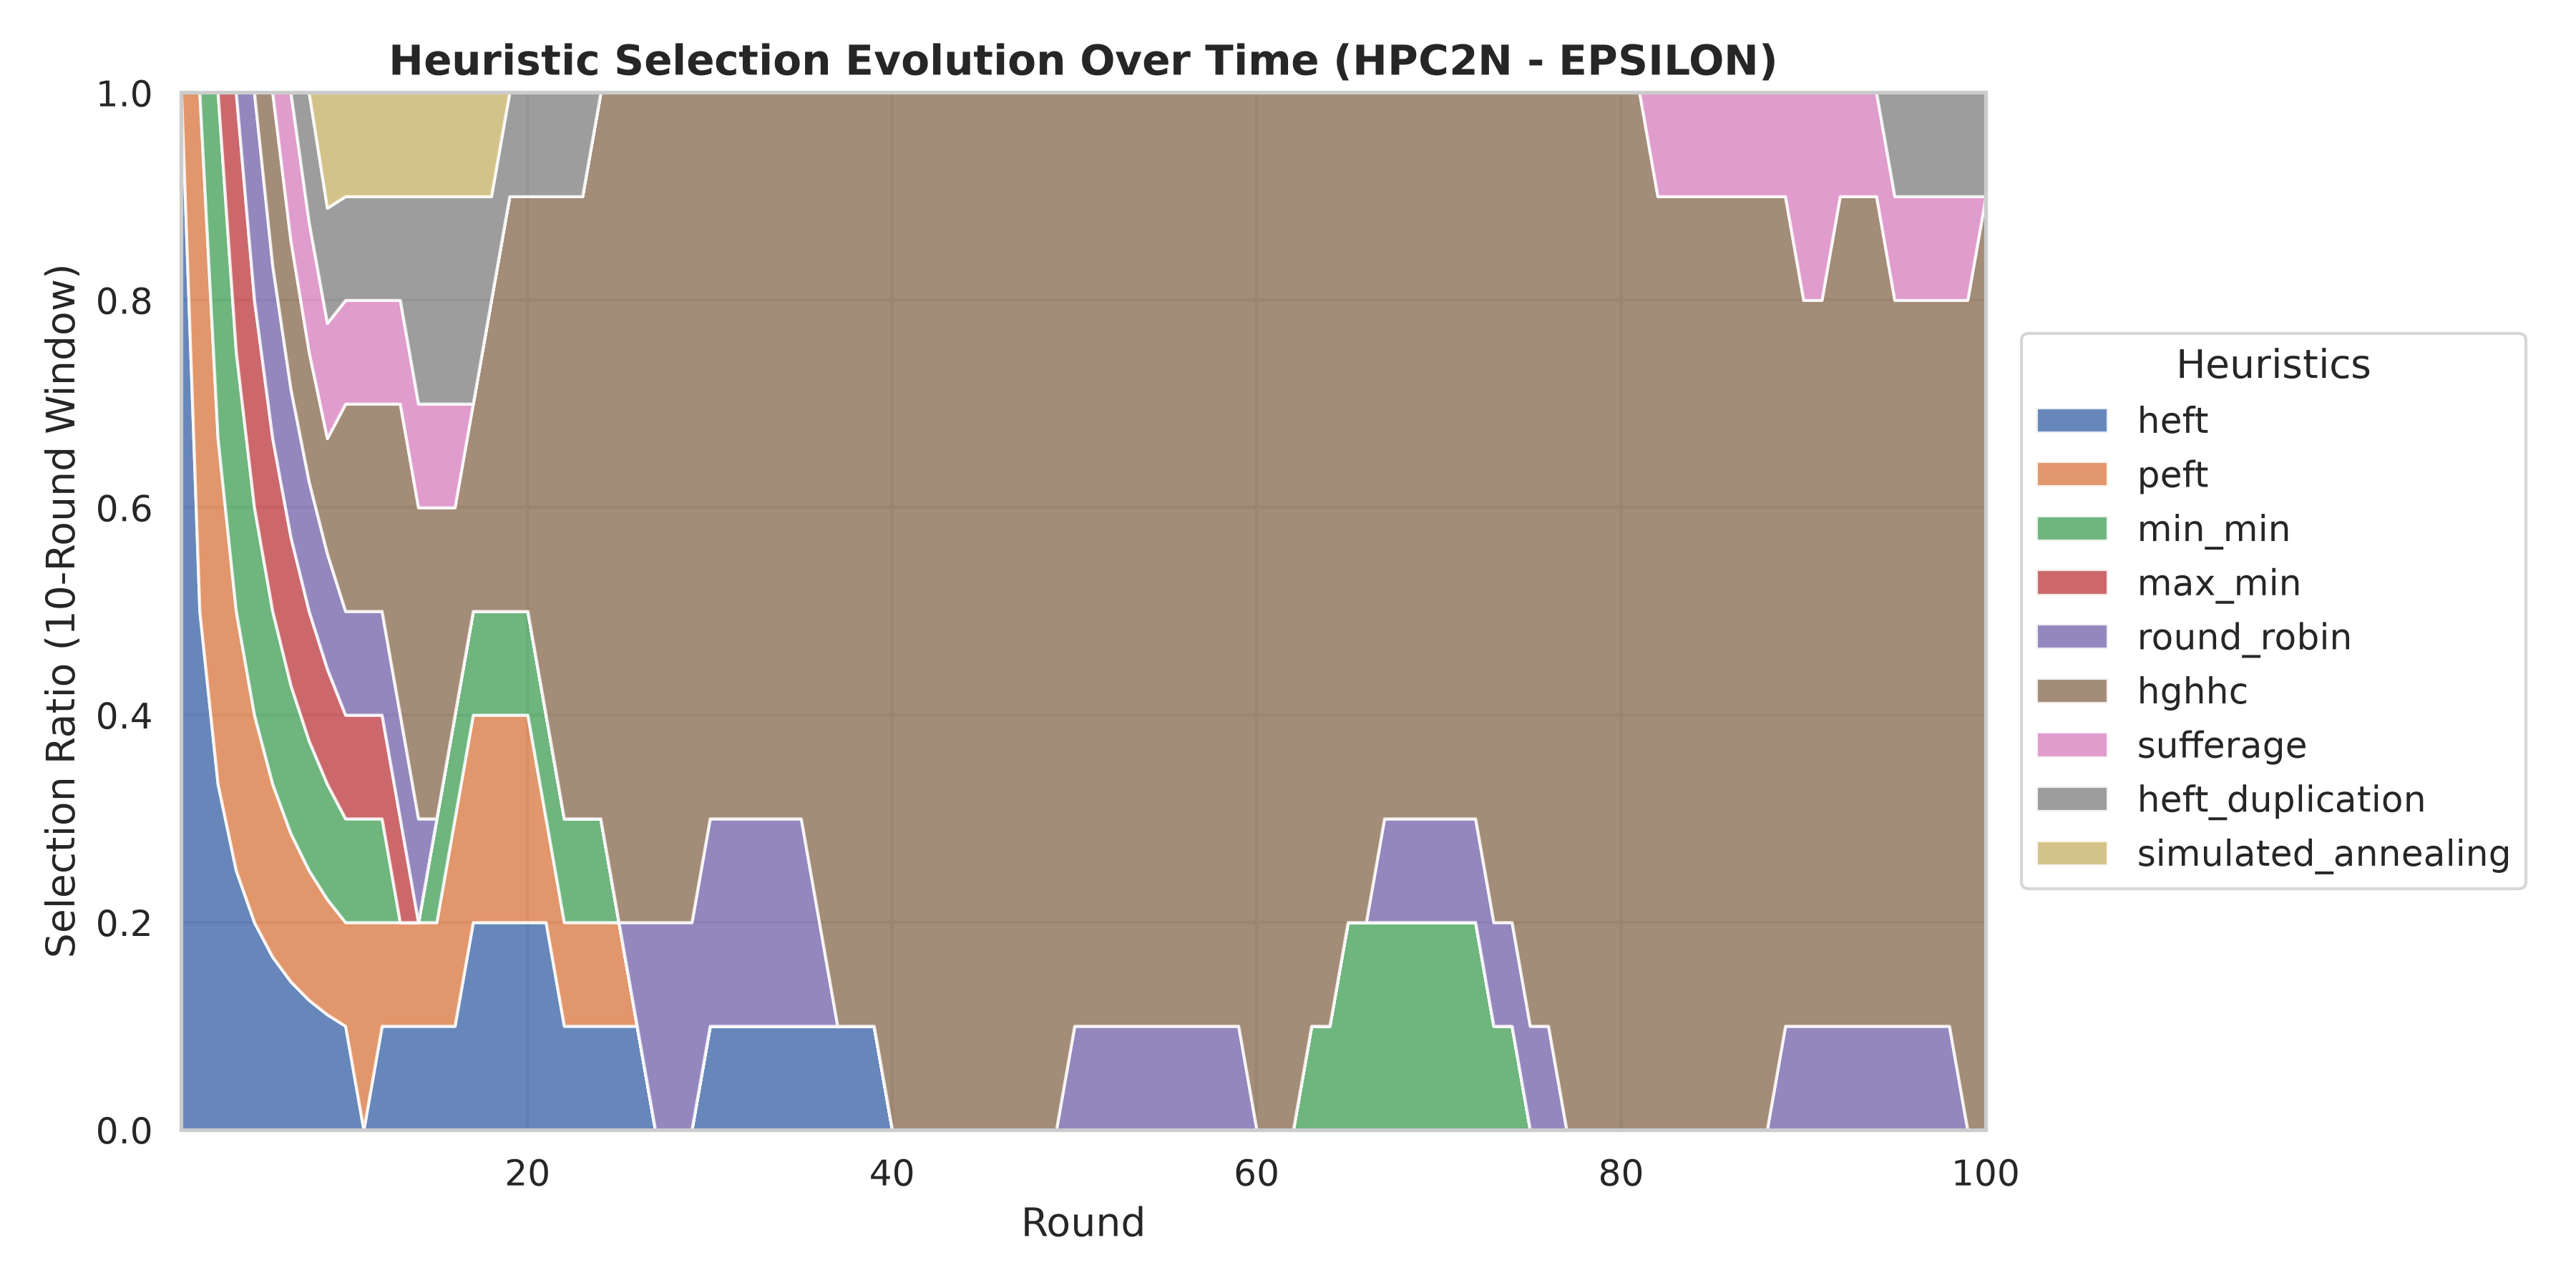
\includegraphics[width=\textwidth]{hpc2n_epsilon_arm_selection_evolution.png}
        \caption{HPC2N -- $\epsilon$-Greedy}
        \label{fig:selection_hpc2n_epsilon}
    \end{subfigure}
    \caption{Low-level heuristic selection ratio evolution over 100 rounds on the HPC2N trace.}
    \label{fig:selection_evolution_hpc2n}
\end{figure}

\begin{figure}[htbp]
    \centering
    \begin{subfigure}[b]{0.48\textwidth}
        \centering
        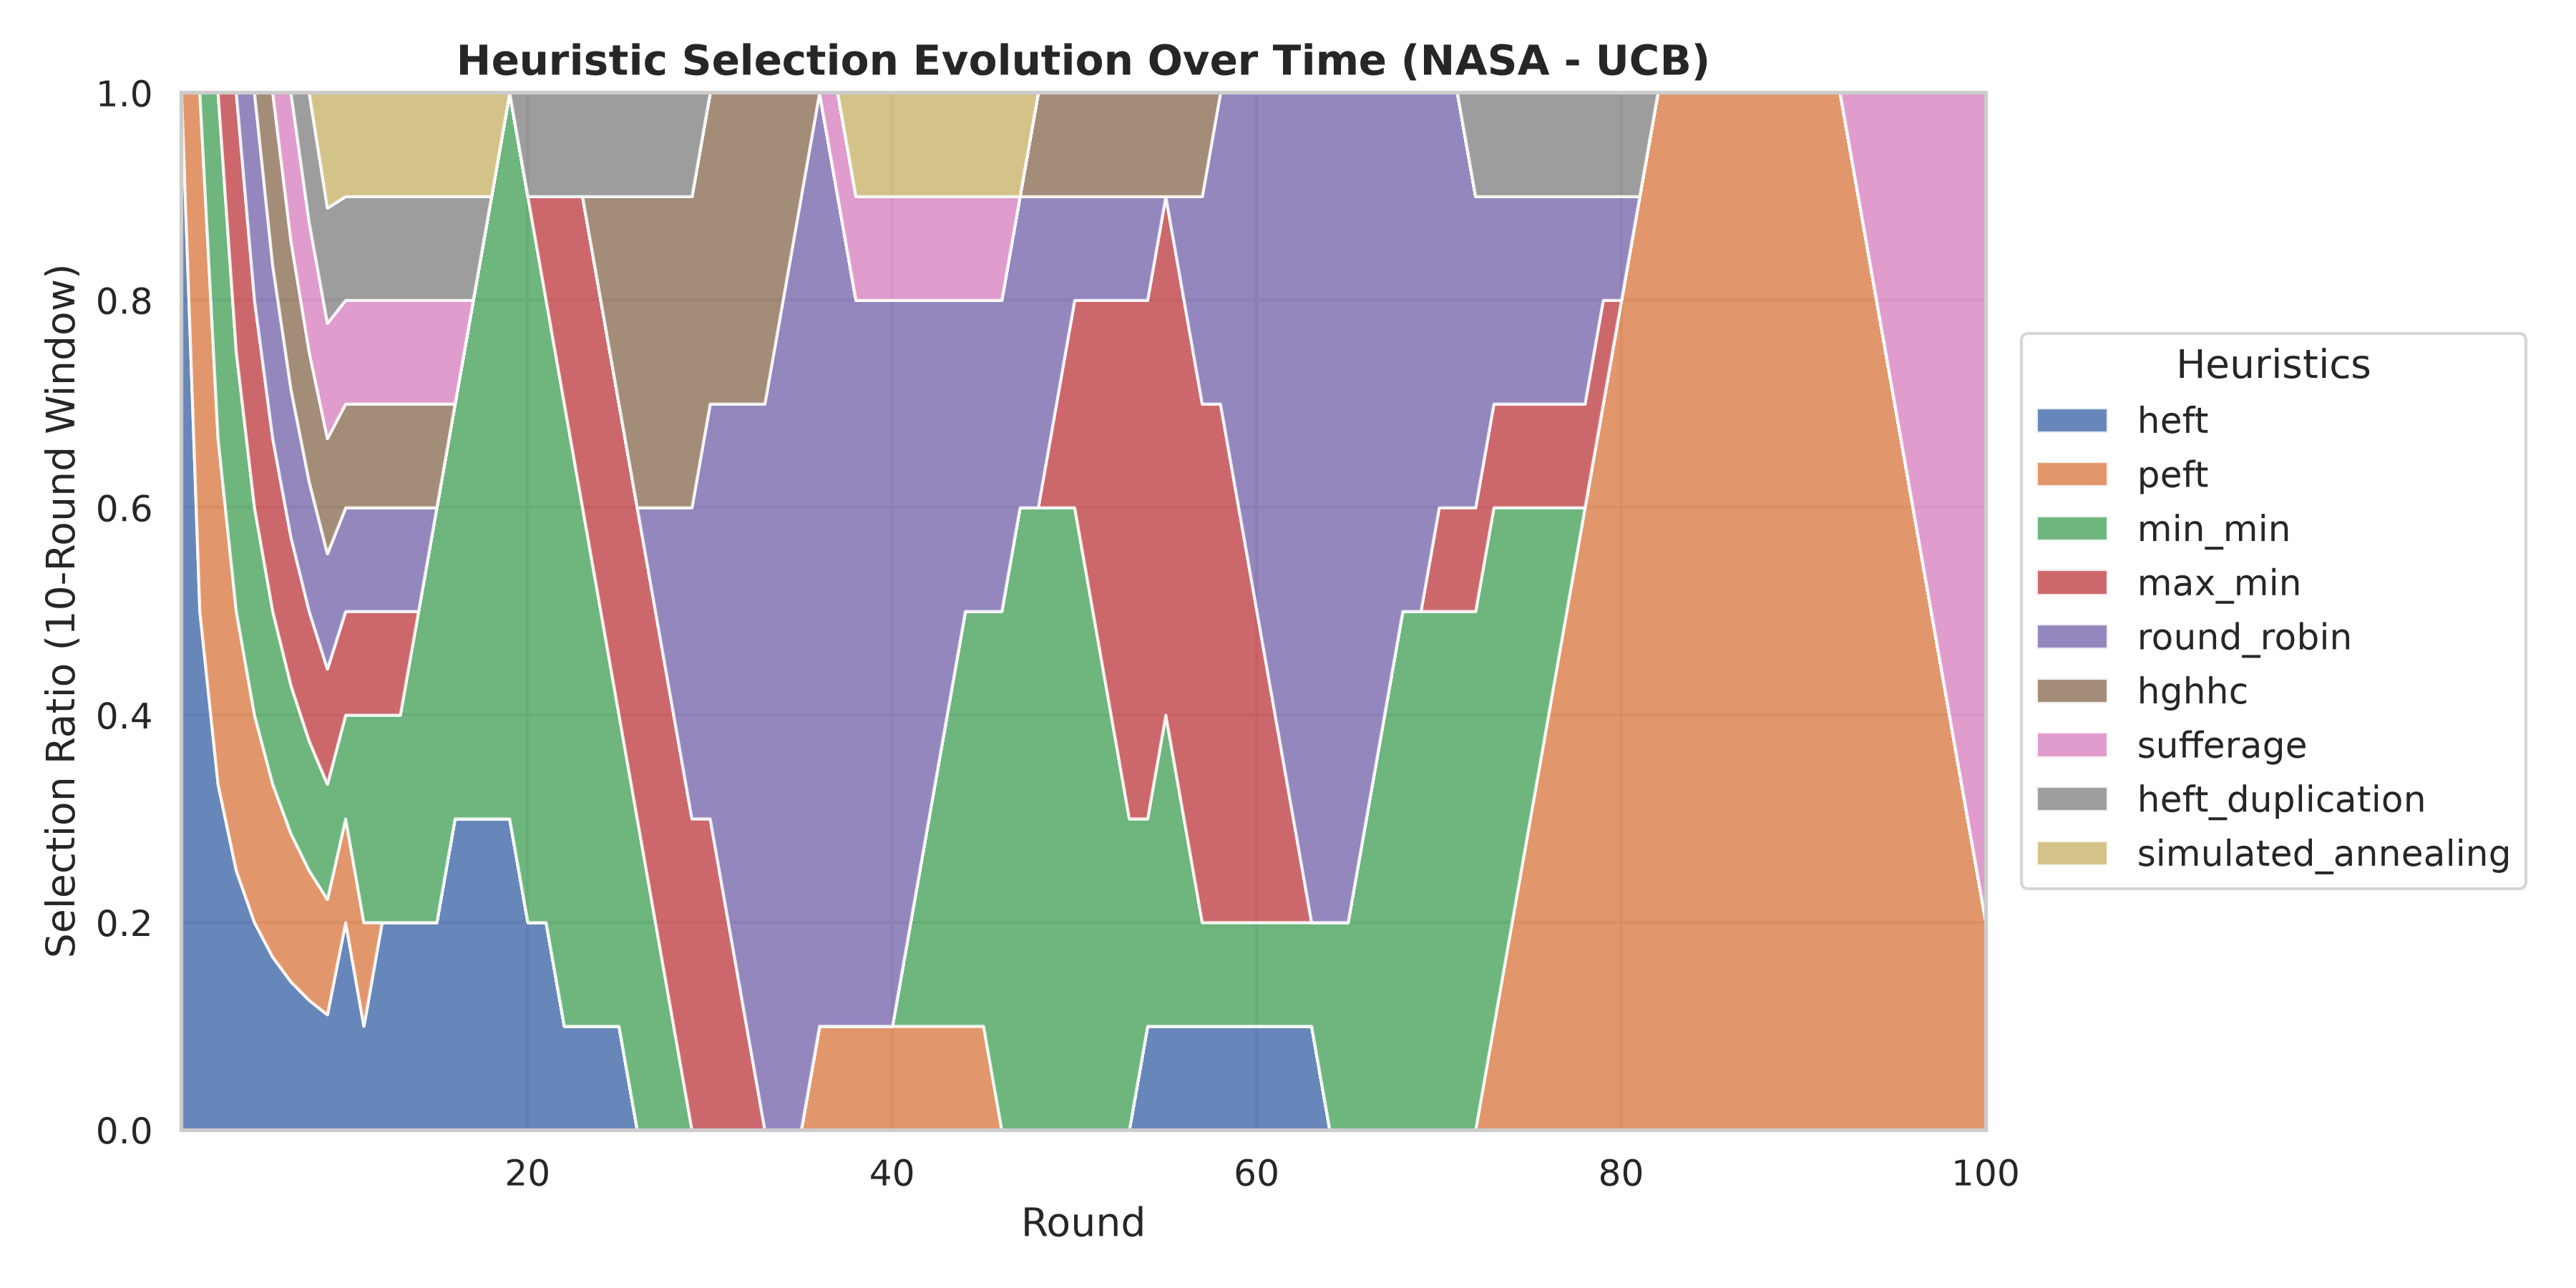
\includegraphics[width=\textwidth]{nasa_ucb_arm_selection_evolution.png}
        \caption{NASA -- UCB}
        \label{fig:selection_nasa_ucb}
    \end{subfigure}
    \hfill
    \begin{subfigure}[b]{0.48\textwidth}
        \centering
        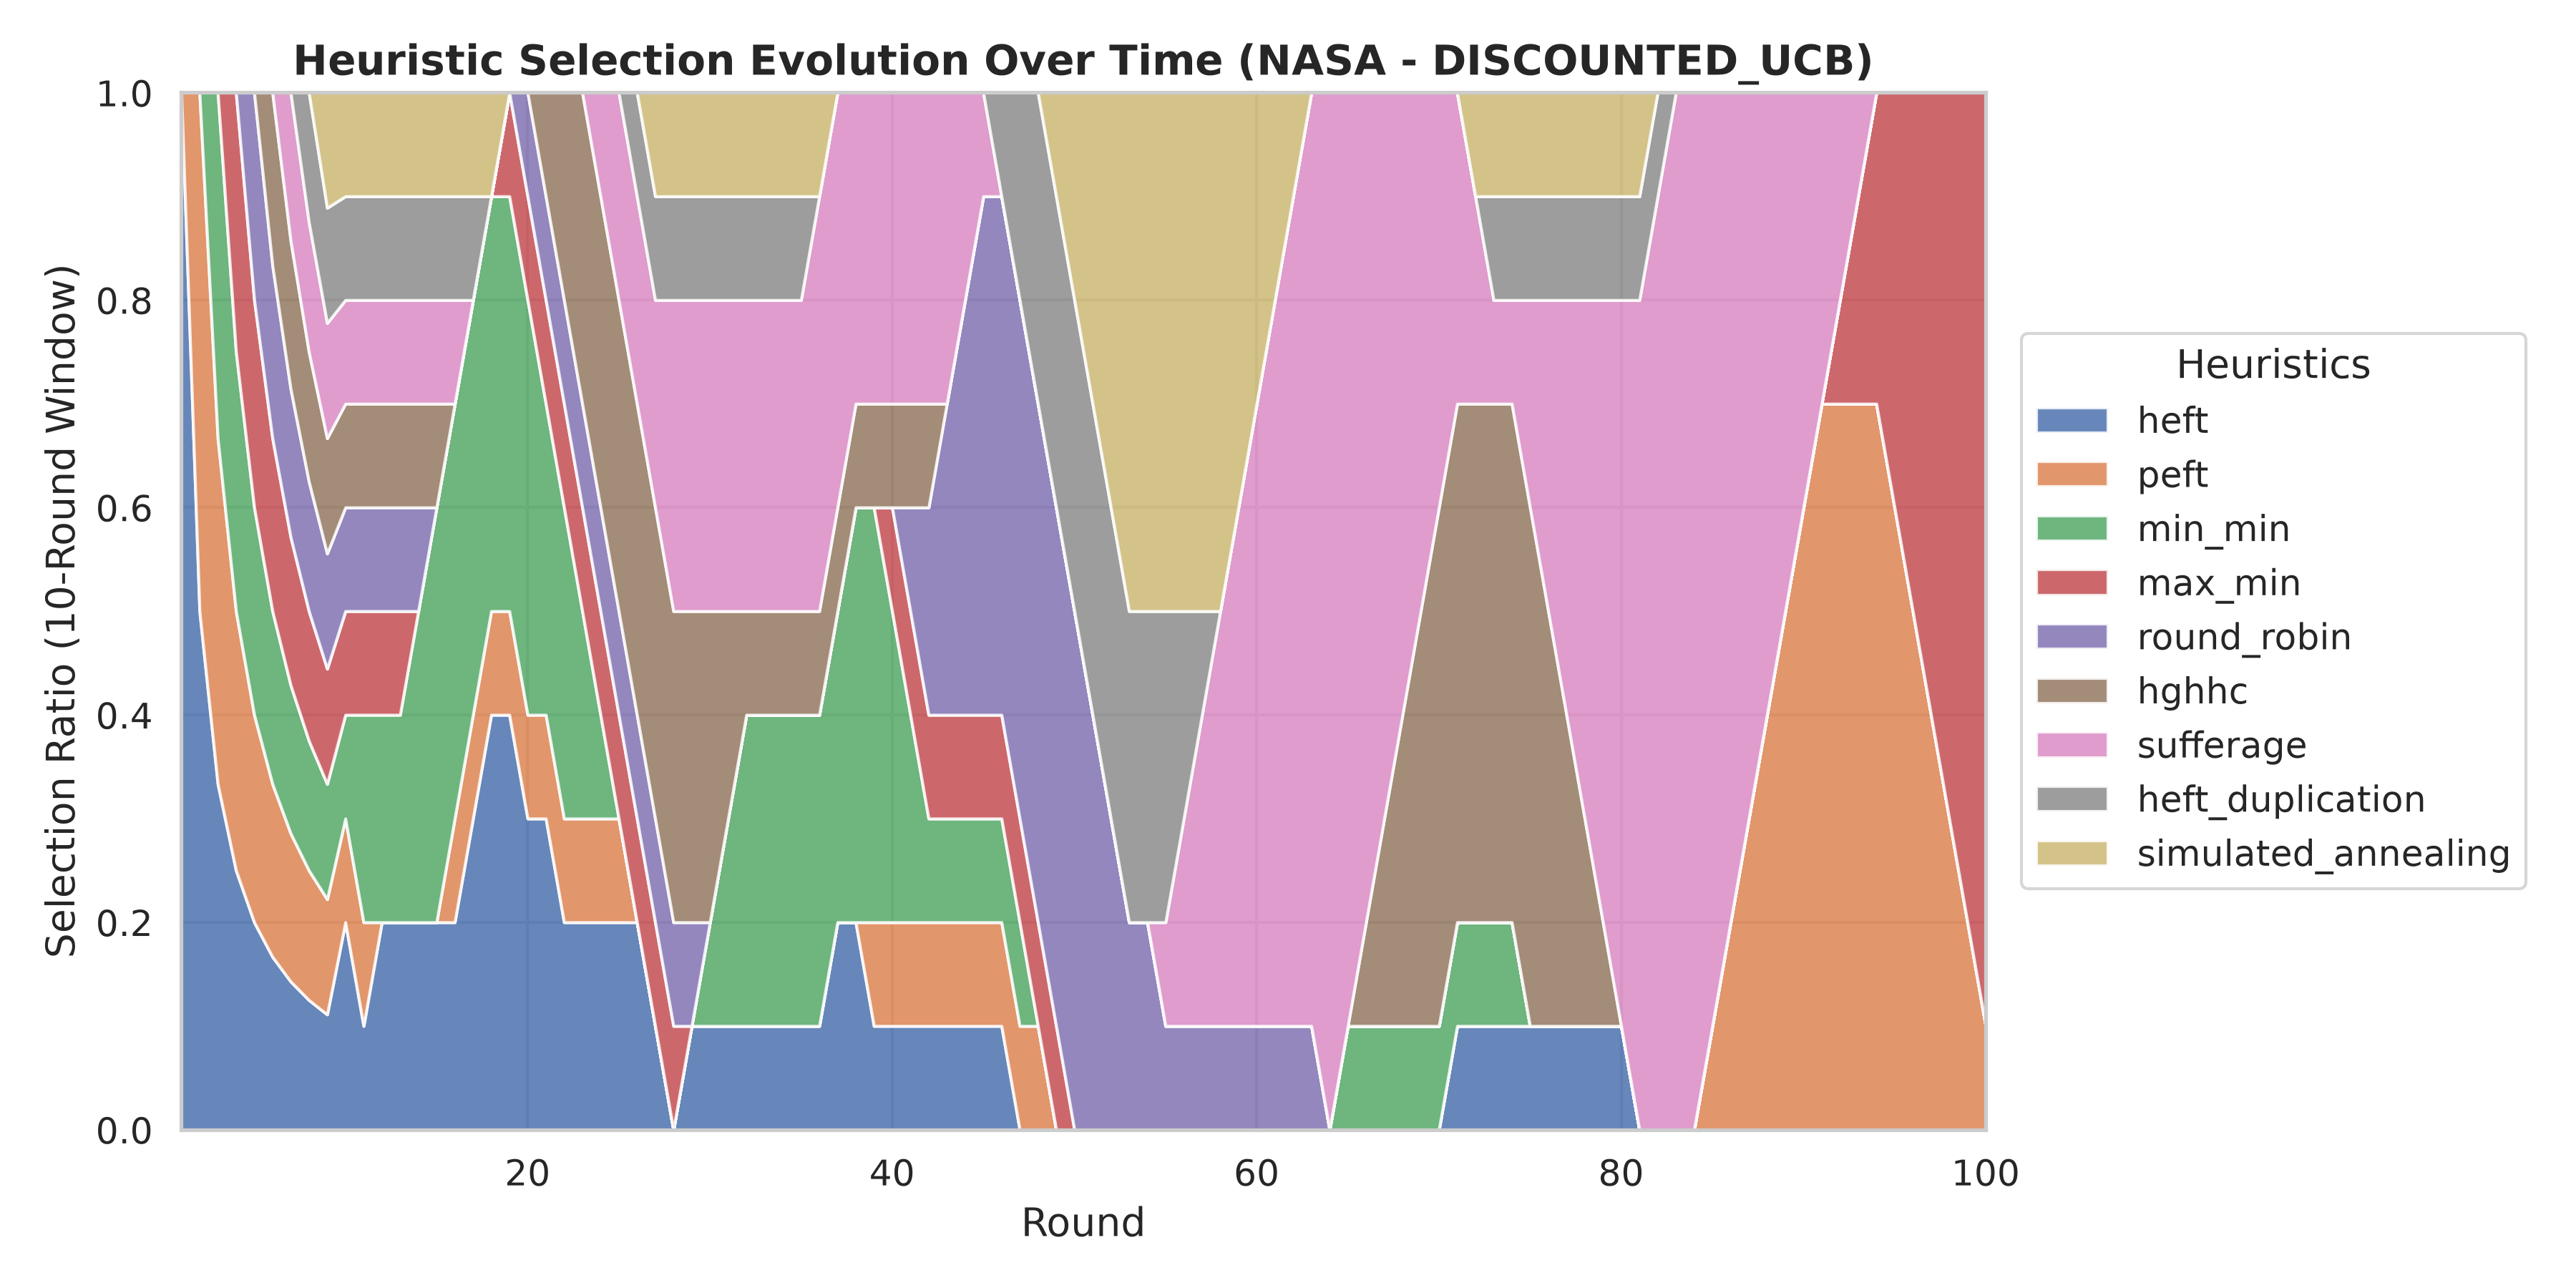
\includegraphics[width=\textwidth]{nasa_discounted_ucb_arm_selection_evolution.png}
        \caption{NASA -- Discounted UCB}
        \label{fig:selection_nasa_discounted}
    \end{subfigure}
    \vskip\baselineskip
    \begin{subfigure}[b]{0.48\textwidth}
        \centering
        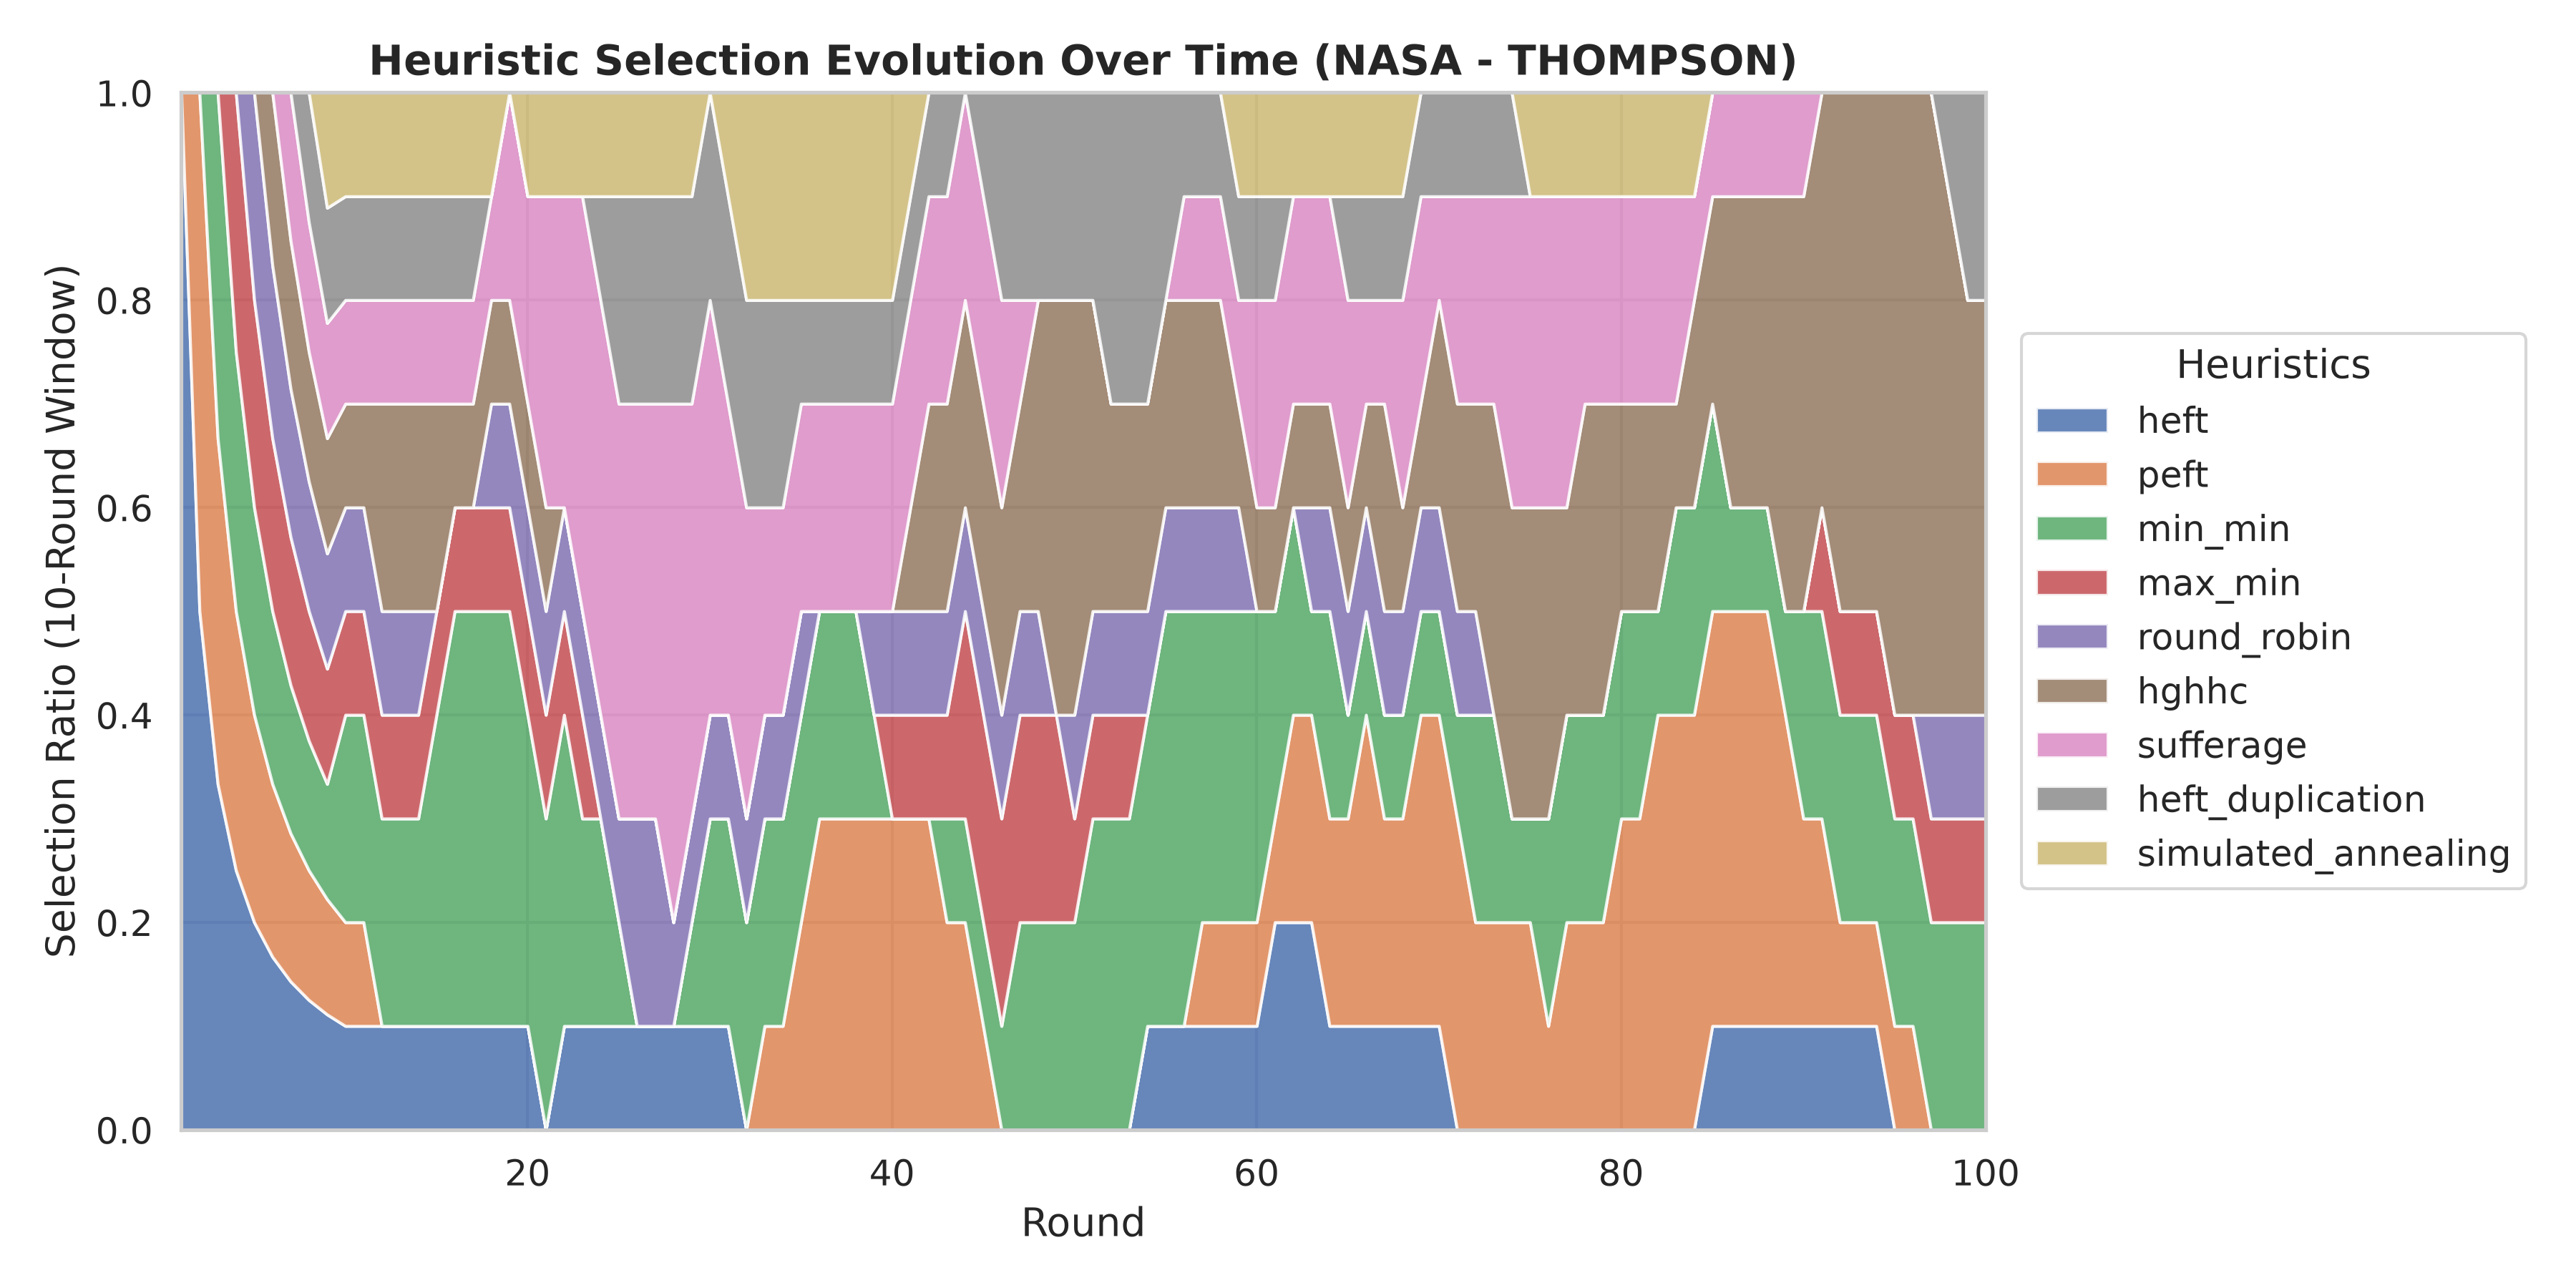
\includegraphics[width=\textwidth]{nasa_thompson_arm_selection_evolution.png}
        \caption{NASA -- Thompson Sampling}
        \label{fig:selection_nasa_epsilon}
    \end{subfigure}
    \hfill
    \begin{subfigure}[b]{0.48\textwidth}
        \centering
        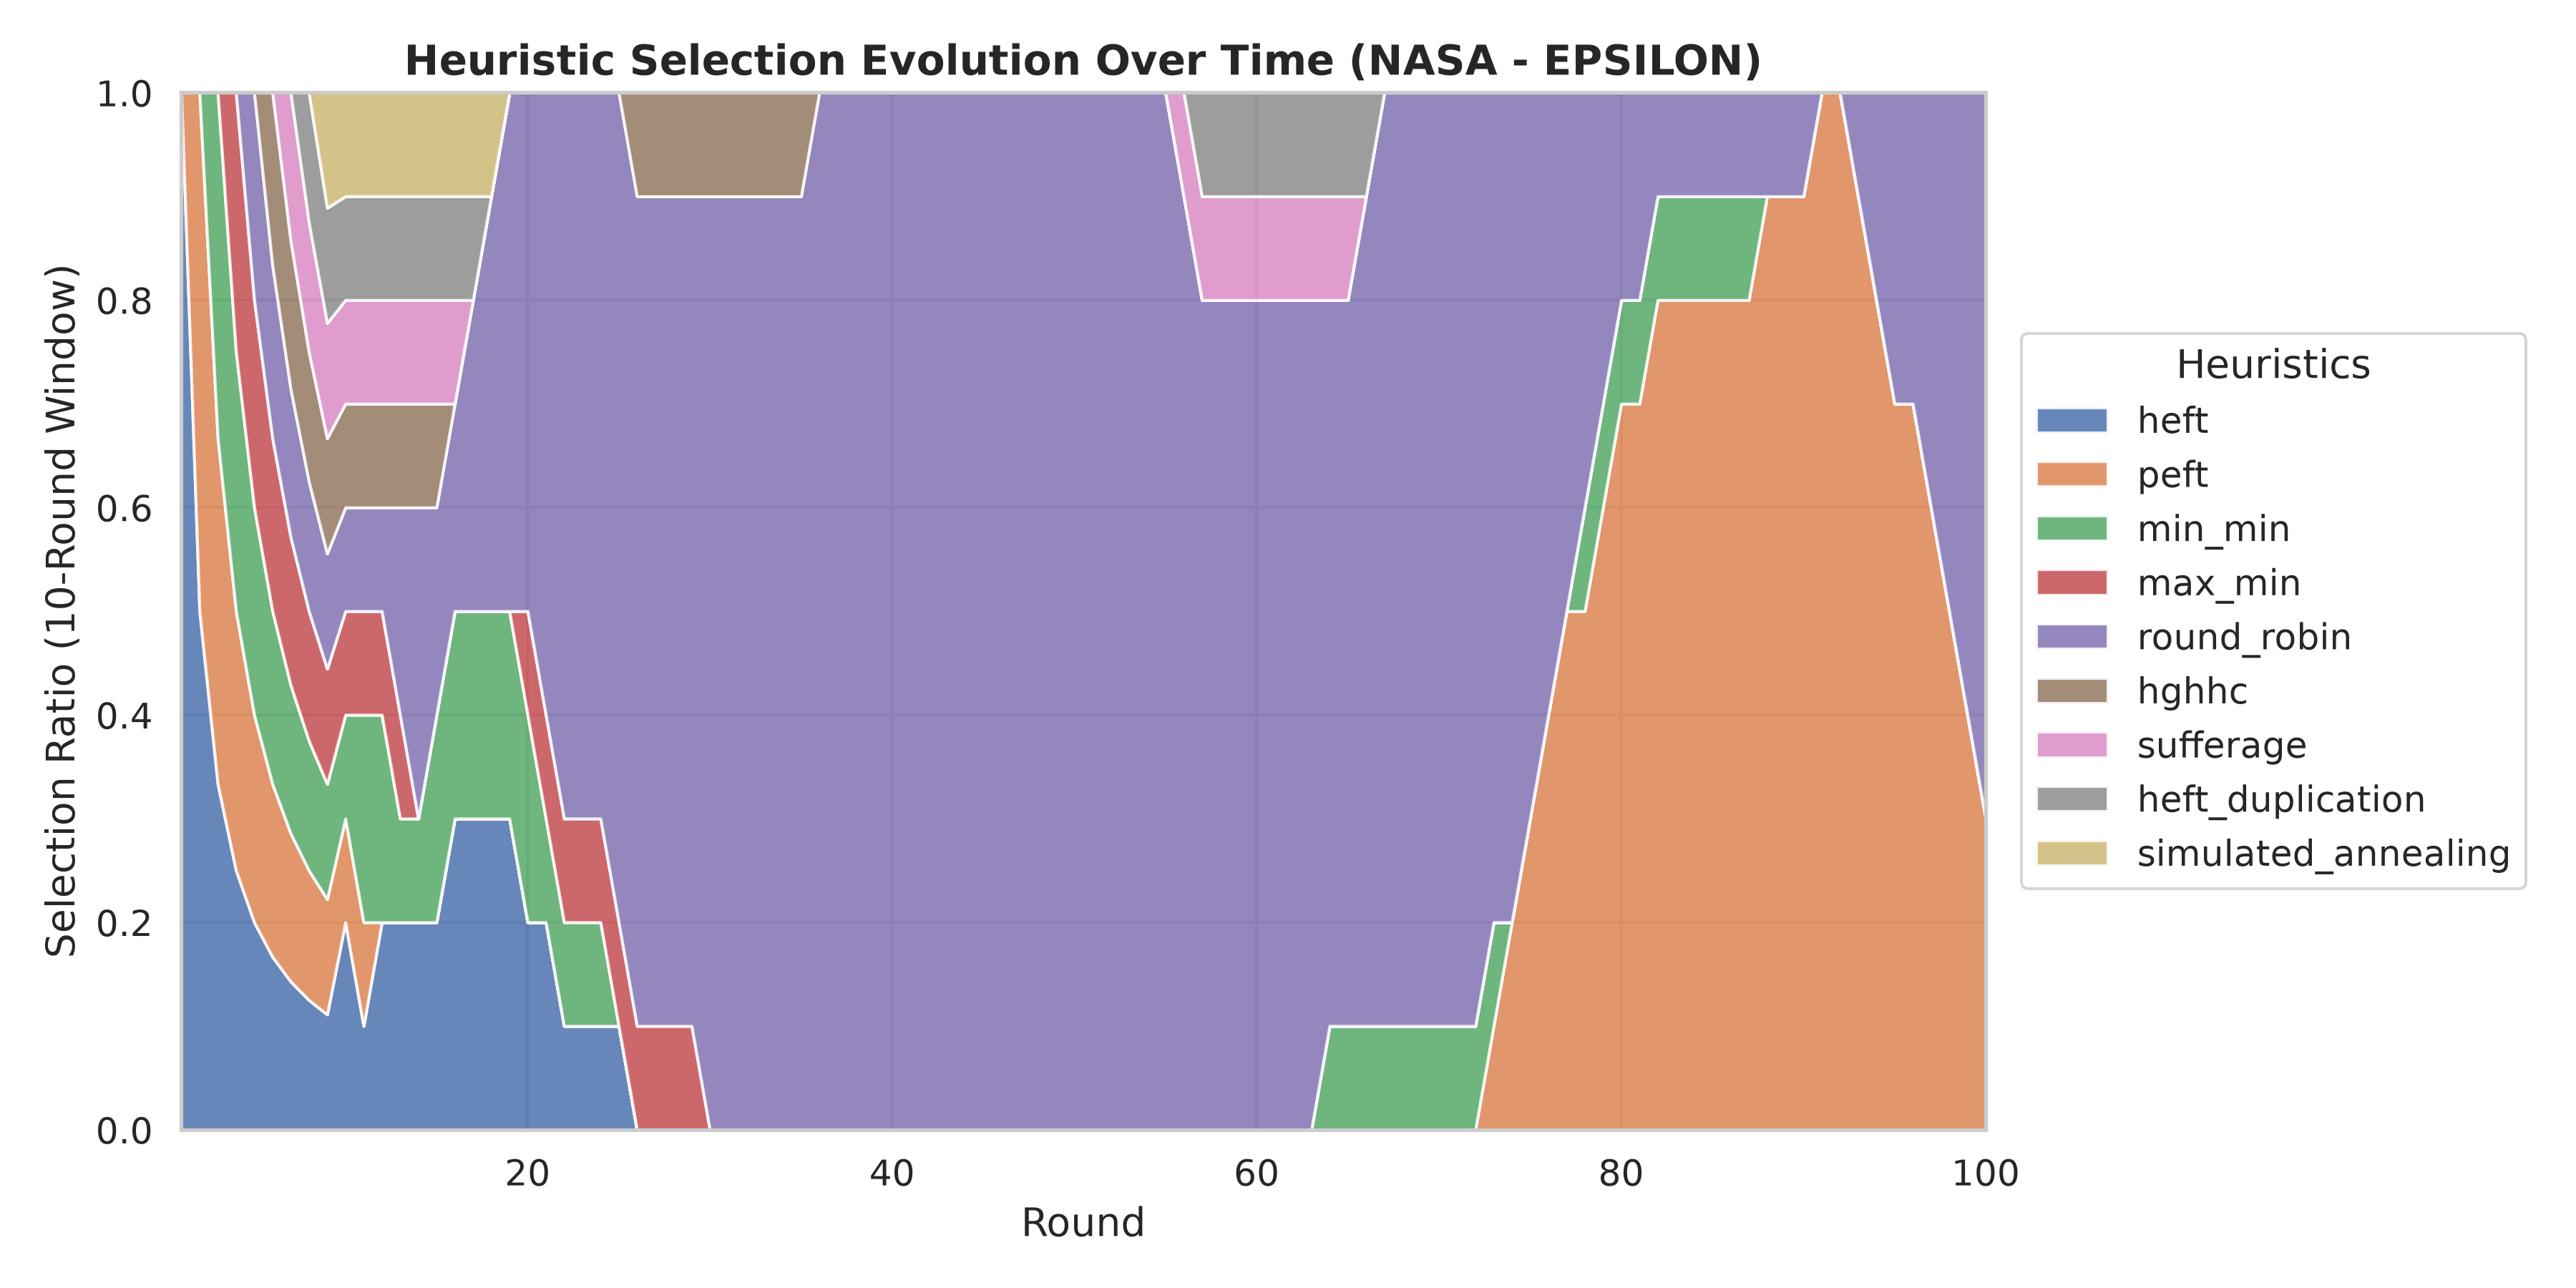
\includegraphics[width=\textwidth]{nasa_epsilon_arm_selection_evolution.png}
        \caption{NASA -- $\epsilon$-Greedy}
        \label{fig:selection_hpc2n_epsilon}
    \end{subfigure}
    \caption{Low-level heuristic selection ratio evolution over 100 rounds on the NASA Ames trace.}
    \label{fig:selection_evolution_nasa}
\end{figure}

\begin{itemize}
    \item \textbf{Initial Exploration Phase ($k \le 10$):} Unbiased initial sampling yields a broad distribution over the selected algorithms
    \item \textbf{Exploitation Regime on HPC2N ($k > 15$):} On the HPC2N trace, UCB (Figure~\ref{fig:selection_hpc2n_ucb}) and Discounted UCB (Figure~\ref{fig:selection_hpc2n_discounted}) heavily exploit \texttt{hghhc}, which occupies up to $80\%$ of selection windows between rounds 40 and 90, while selectively triggering \texttt{heft} and \texttt{peft} during workload shifts around round 65 and 95. Thompson Sampling (Figure~\ref{fig:selection_hpc2n_thompson}) maintains a more continuous sampling spread between \texttt{hghhc}, \texttt{peft}, and \texttt{sufferage}.
    \item \textbf{Phase Lock on NASA Ames:} On the NASA Ames trace, UCB (Figure~\ref{fig:selection_nasa_ucb}) locks onto \texttt{round\_robin} and \texttt{max\_min} between rounds 30 and 60 before transitioning to \texttt{peft}. Discounted UCB (Figure~\ref{fig:selection_nasa_discounted}) dynamically shuffles between \texttt{sufferage}, \texttt{simulated\_annealing}, \texttt{hghhc}, and \texttt{peft}, which prevents a premature policy saturation in highly uniform arrival regimes.
\end{itemize}

\subsubsection{Cumulative Makespan Trajectories}
Figures~\ref{fig:makespan_hpc2n_all} and~\ref{fig:makespan_nasa_all} showcase the cumulative makespan curves across all four bandit implementations against standalone baseline heuristics.

\begin{figure}[htbp]
    \centering
    \begin{subfigure}[b]{0.48\textwidth}
        \centering
        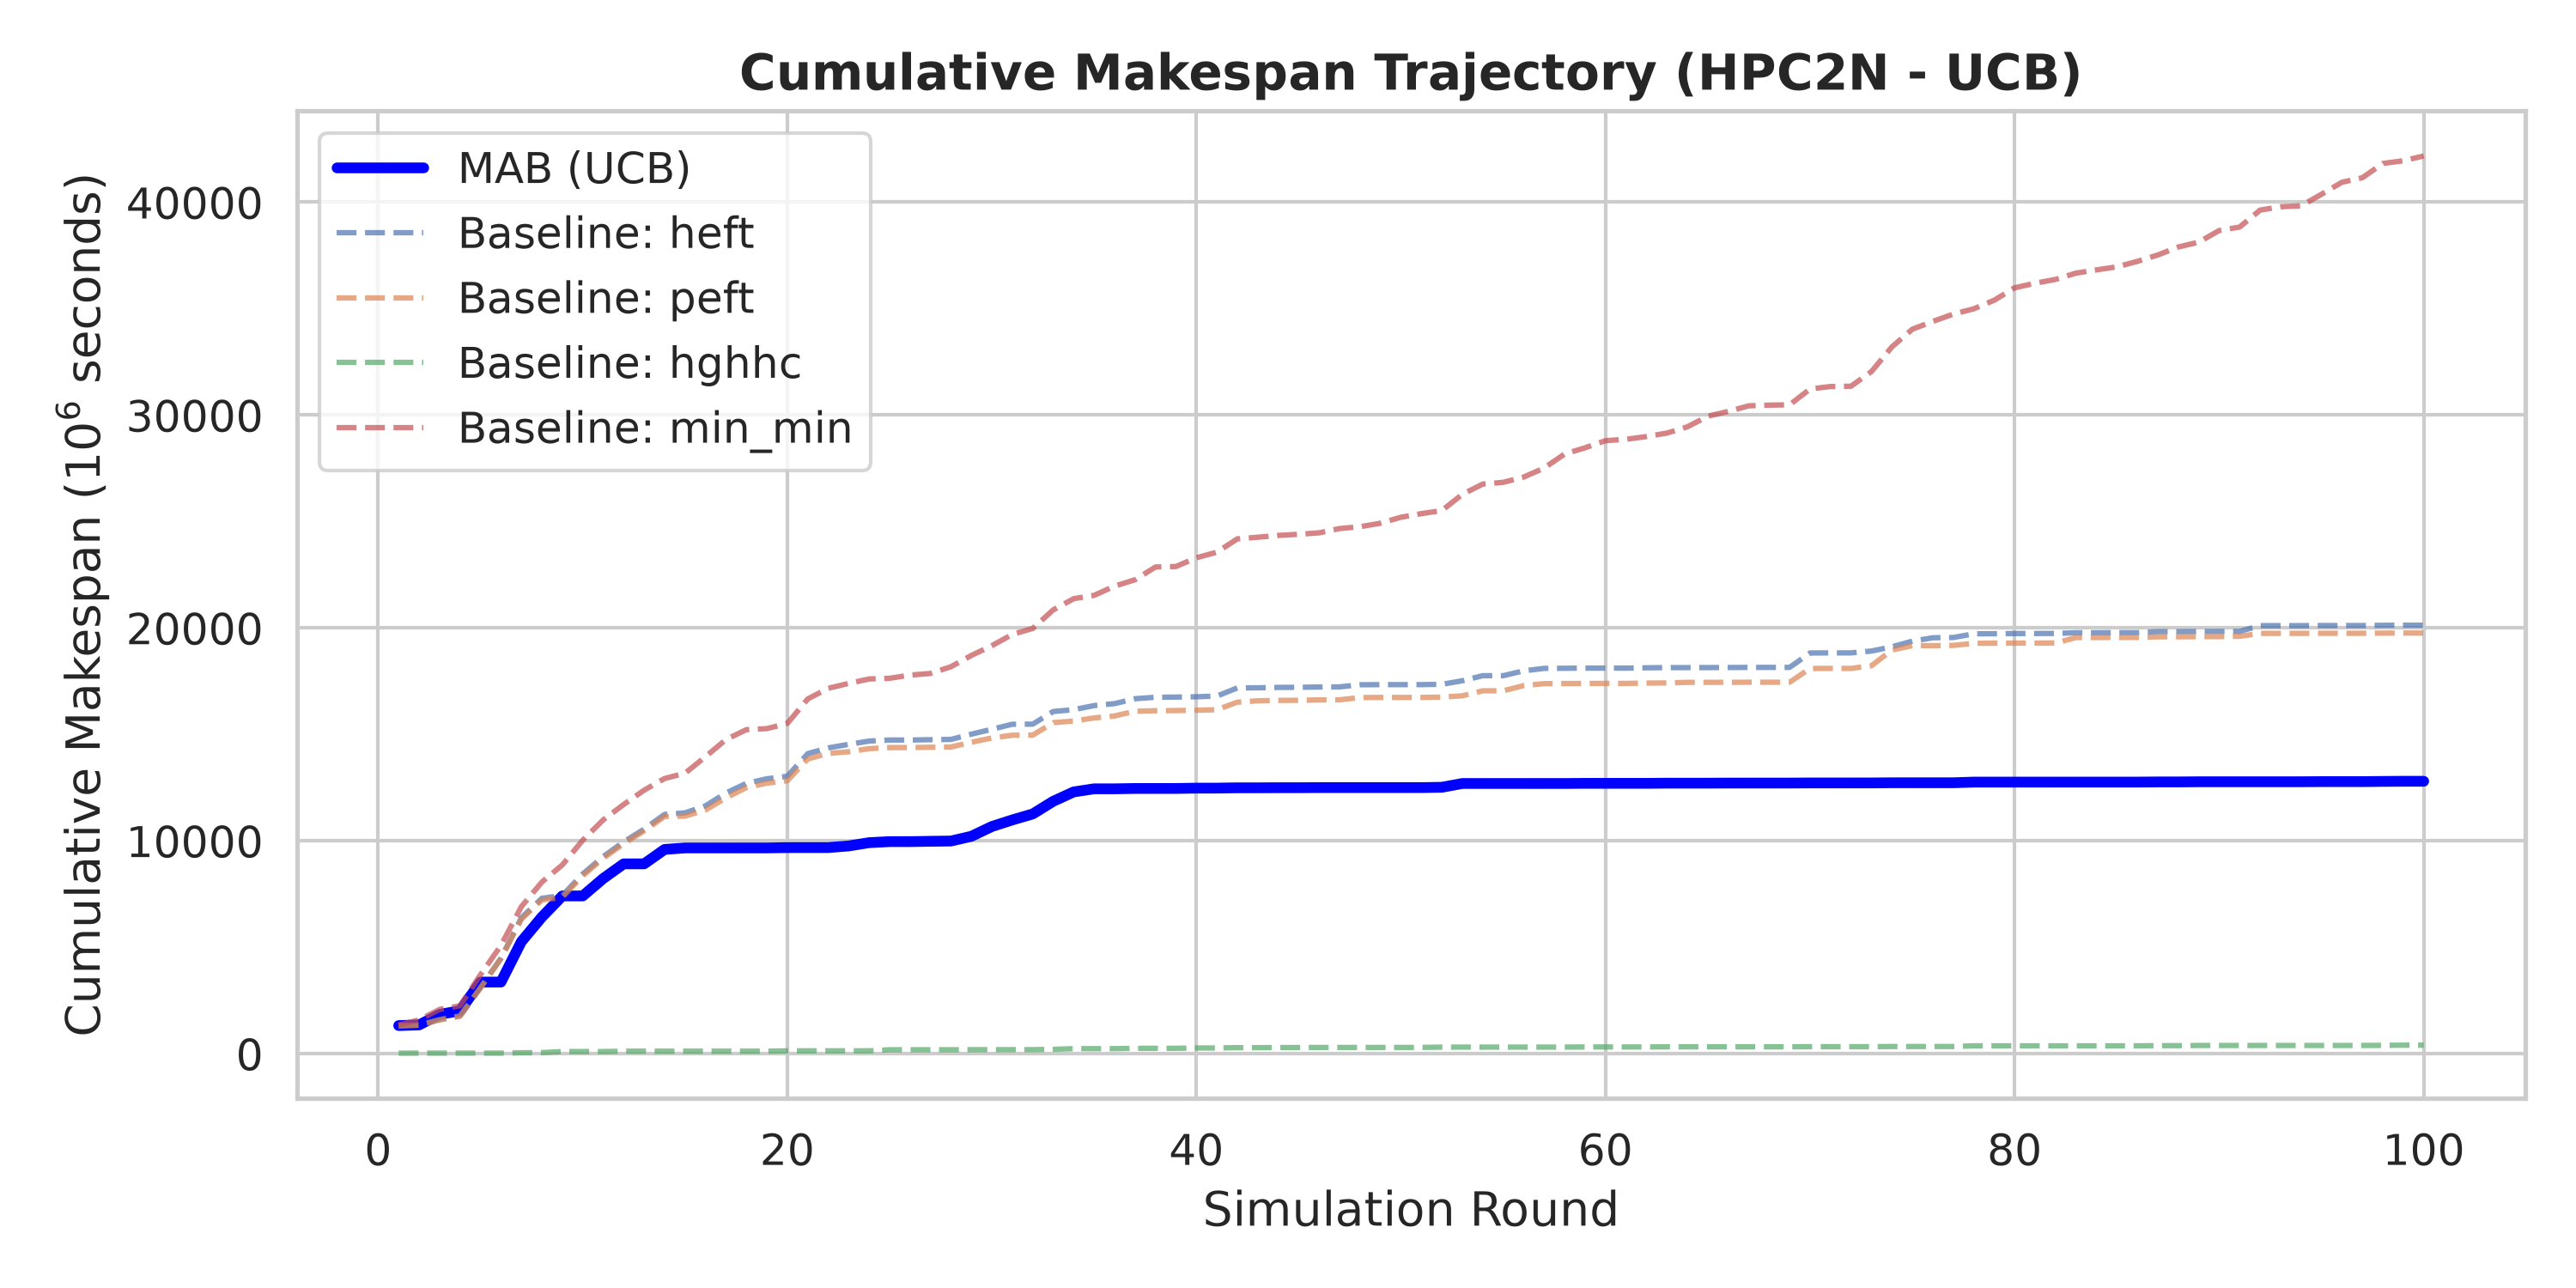
\includegraphics[width=\textwidth]{hpc2n_ucb_cumulative_makespan.png}
        \caption{HPC2N -- UCB}
        \label{fig:makespan_hpc2n_ucb}
    \end{subfigure}
    \hfill
    \begin{subfigure}[b]{0.48\textwidth}
        \centering
        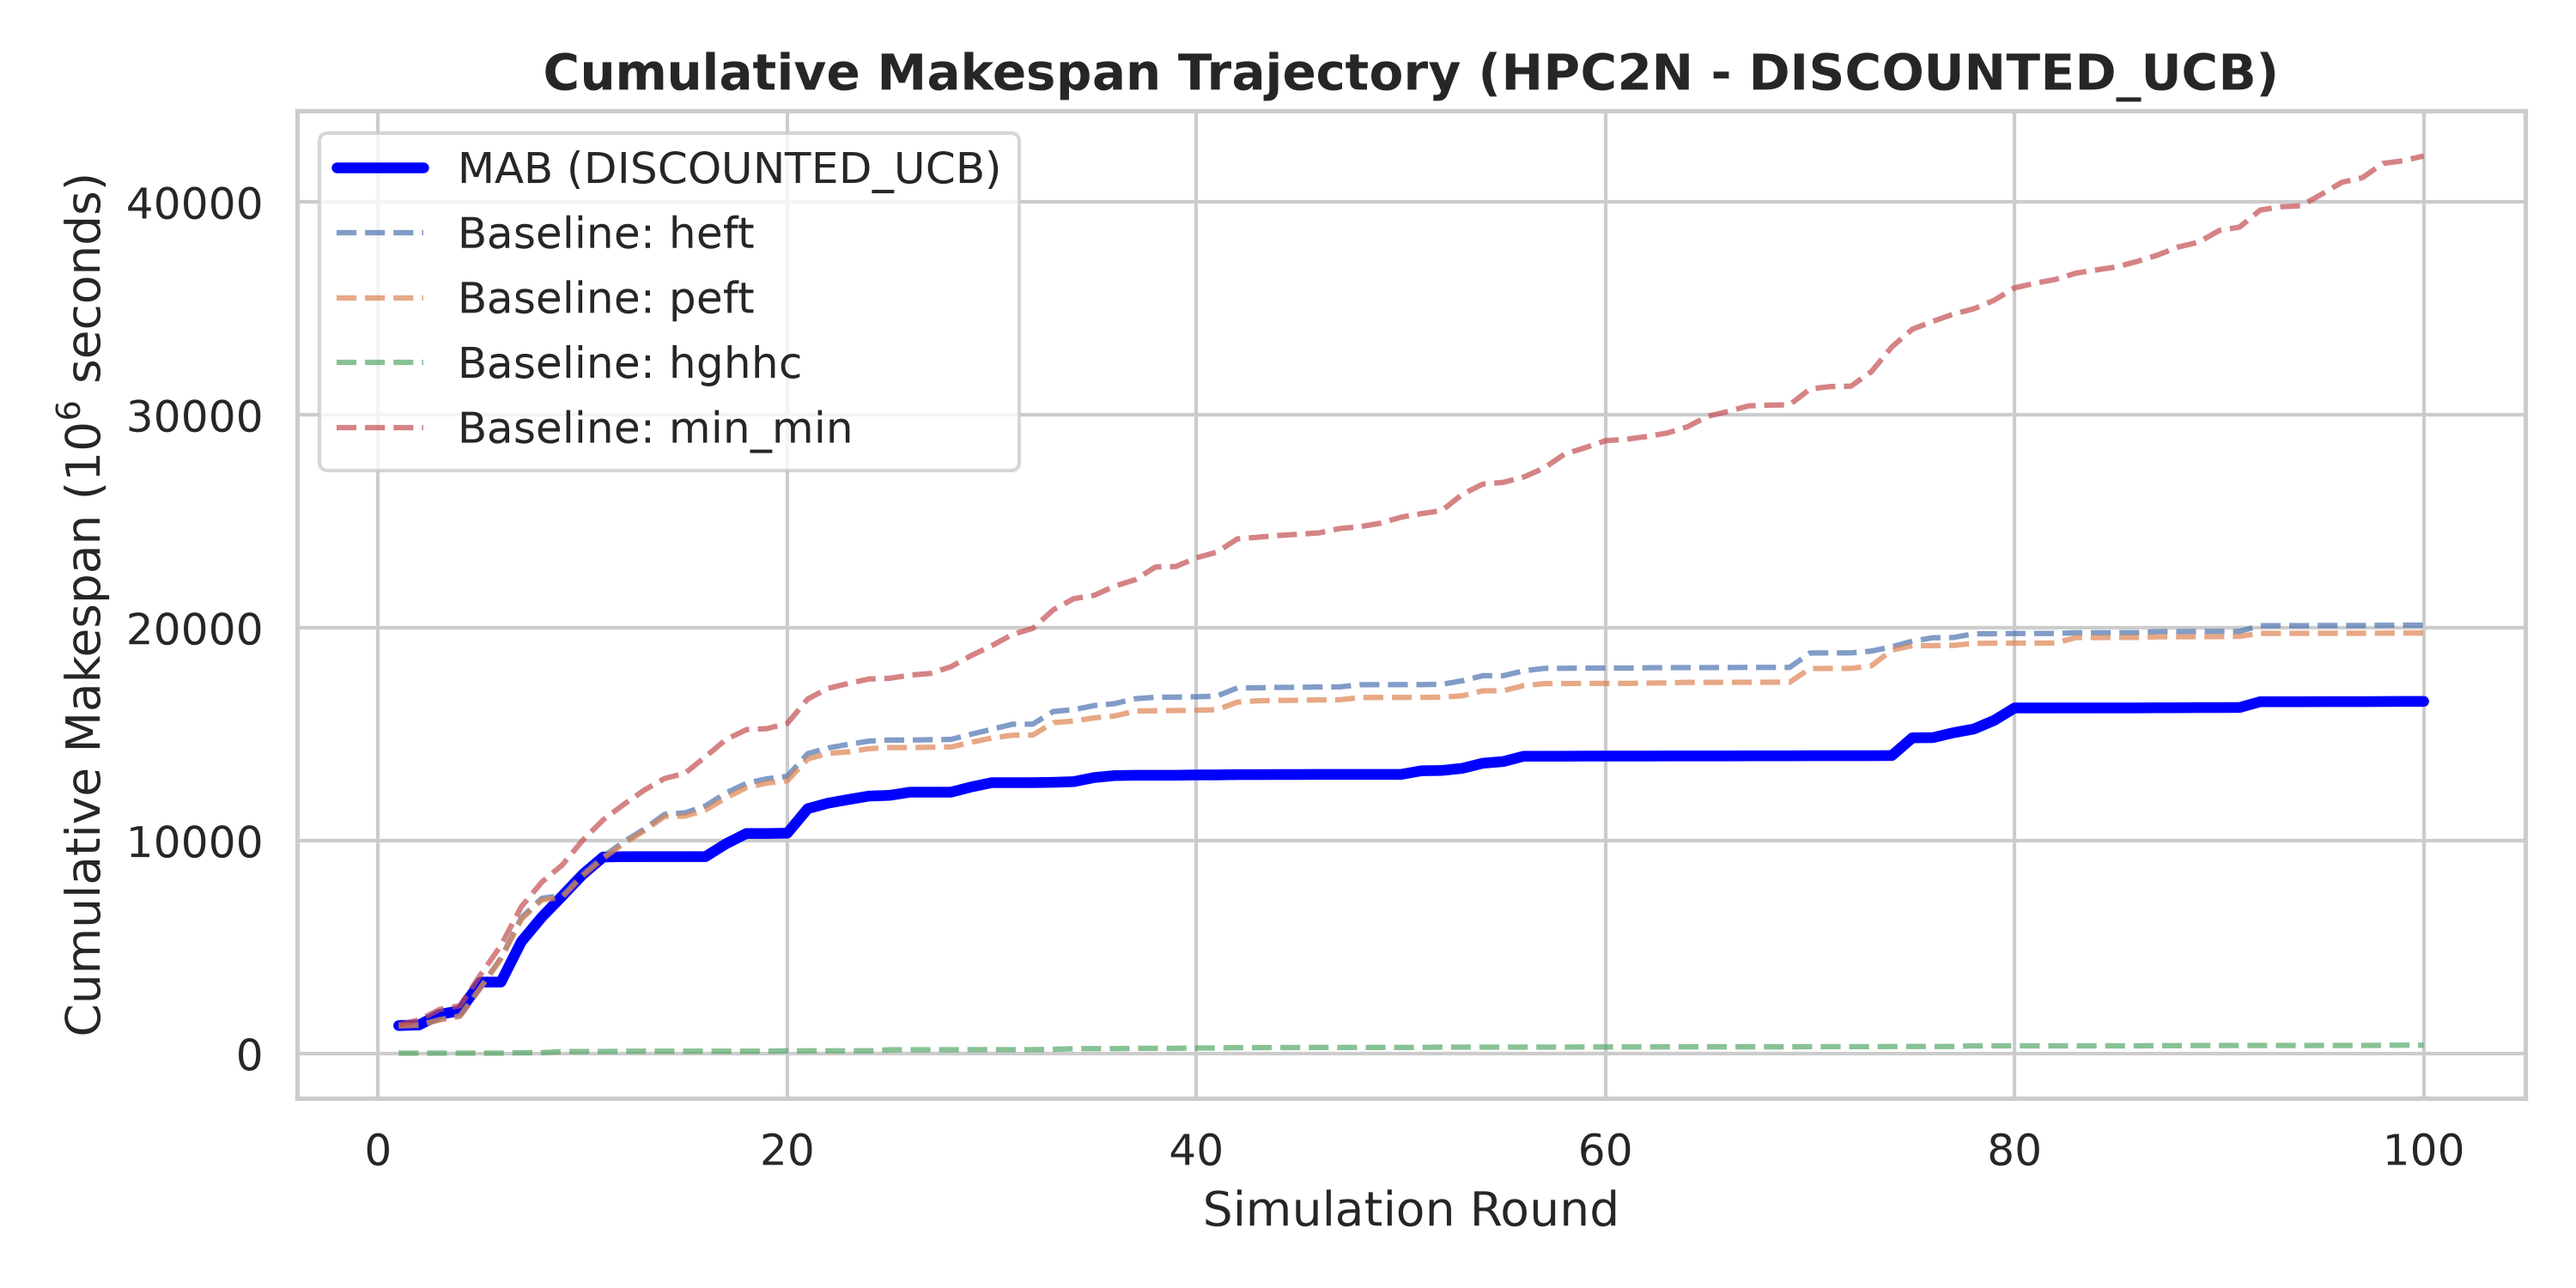
\includegraphics[width=\textwidth]{hpc2n_discounted_ucb_cumulative_makespan.png}
        \caption{HPC2N -- Discounted UCB}
        \label{fig:makespan_hpc2n_discounted}
    \end{subfigure}
    \vskip\baselineskip
    \begin{subfigure}[b]{0.48\textwidth}
        \centering
        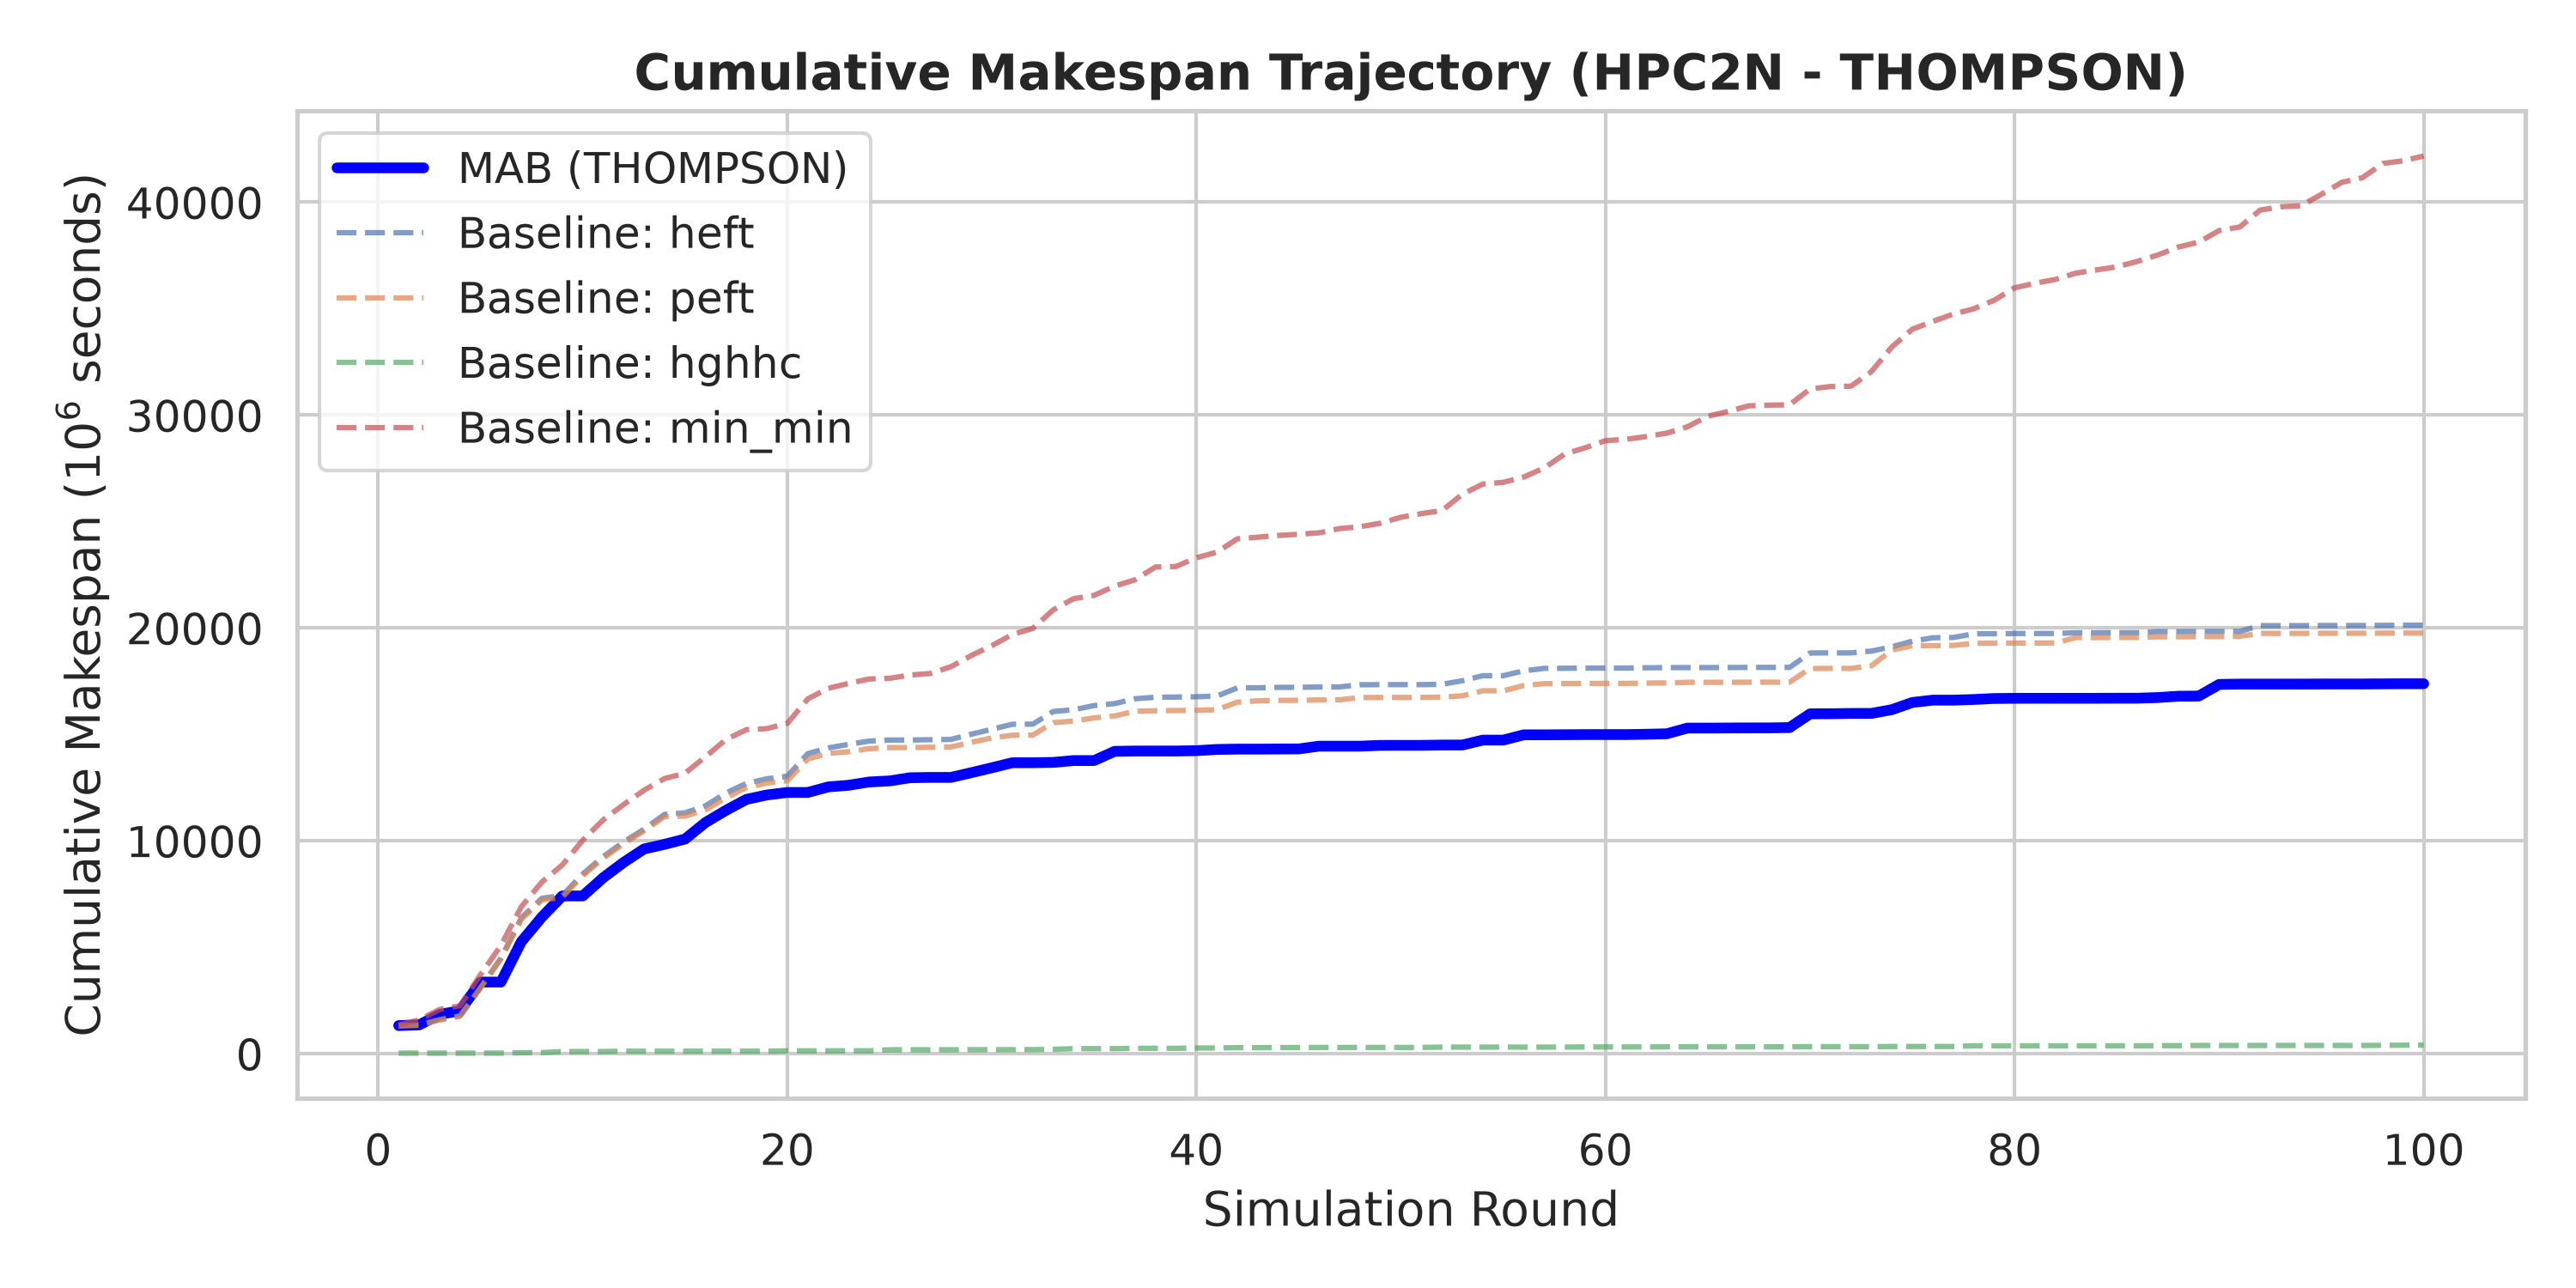
\includegraphics[width=\textwidth]{hpc2n_thompson_cumulative_makespan.png}
        \caption{HPC2N -- Thompson Sampling}
        \label{fig:makespan_hpc2n_thompson}
    \end{subfigure}
    \hfill
    \begin{subfigure}[b]{0.48\textwidth}
        \centering
        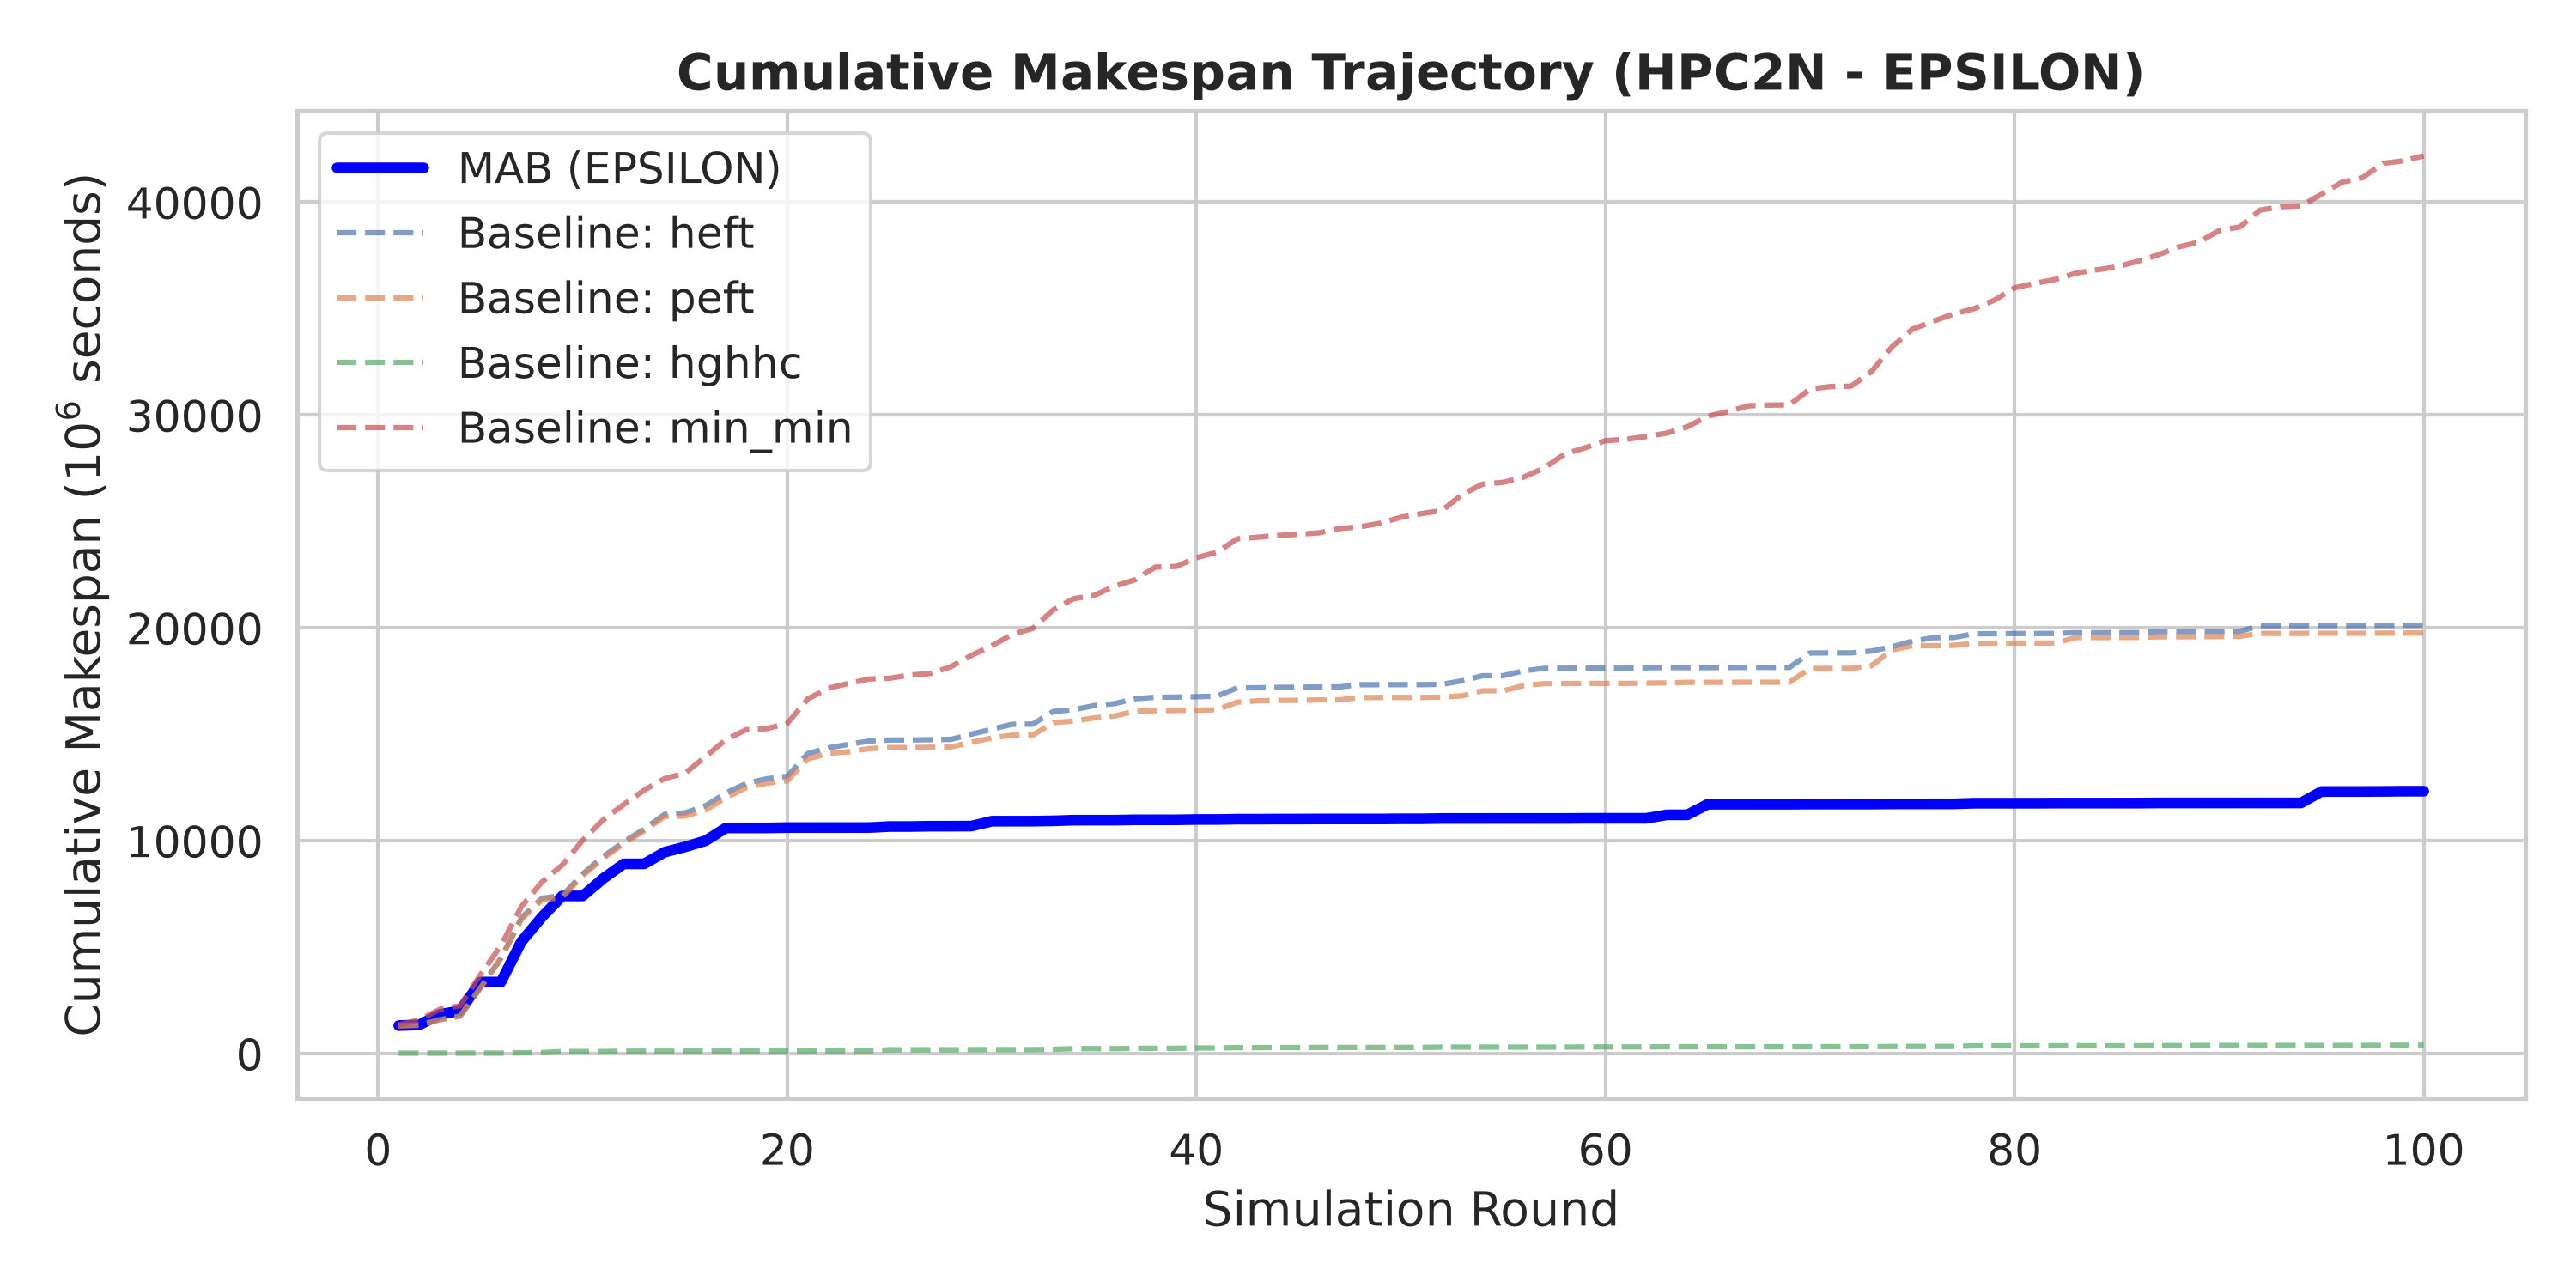
\includegraphics[width=\textwidth]{hpc2n_epsilon_cumulative_makespan.png}
        \caption{HPC2N -- $\epsilon$-Greedy}
        \label{fig:makespan_hpc2n_epsilon}
    \end{subfigure}
    \caption{Cumulative makespan trajectories across MAB variants on the HPC2N workload.}
    \label{fig:makespan_hpc2n_all}
\end{figure}

\begin{figure}[htbp]
    \centering
    \begin{subfigure}[b]{0.48\textwidth}
        \centering
        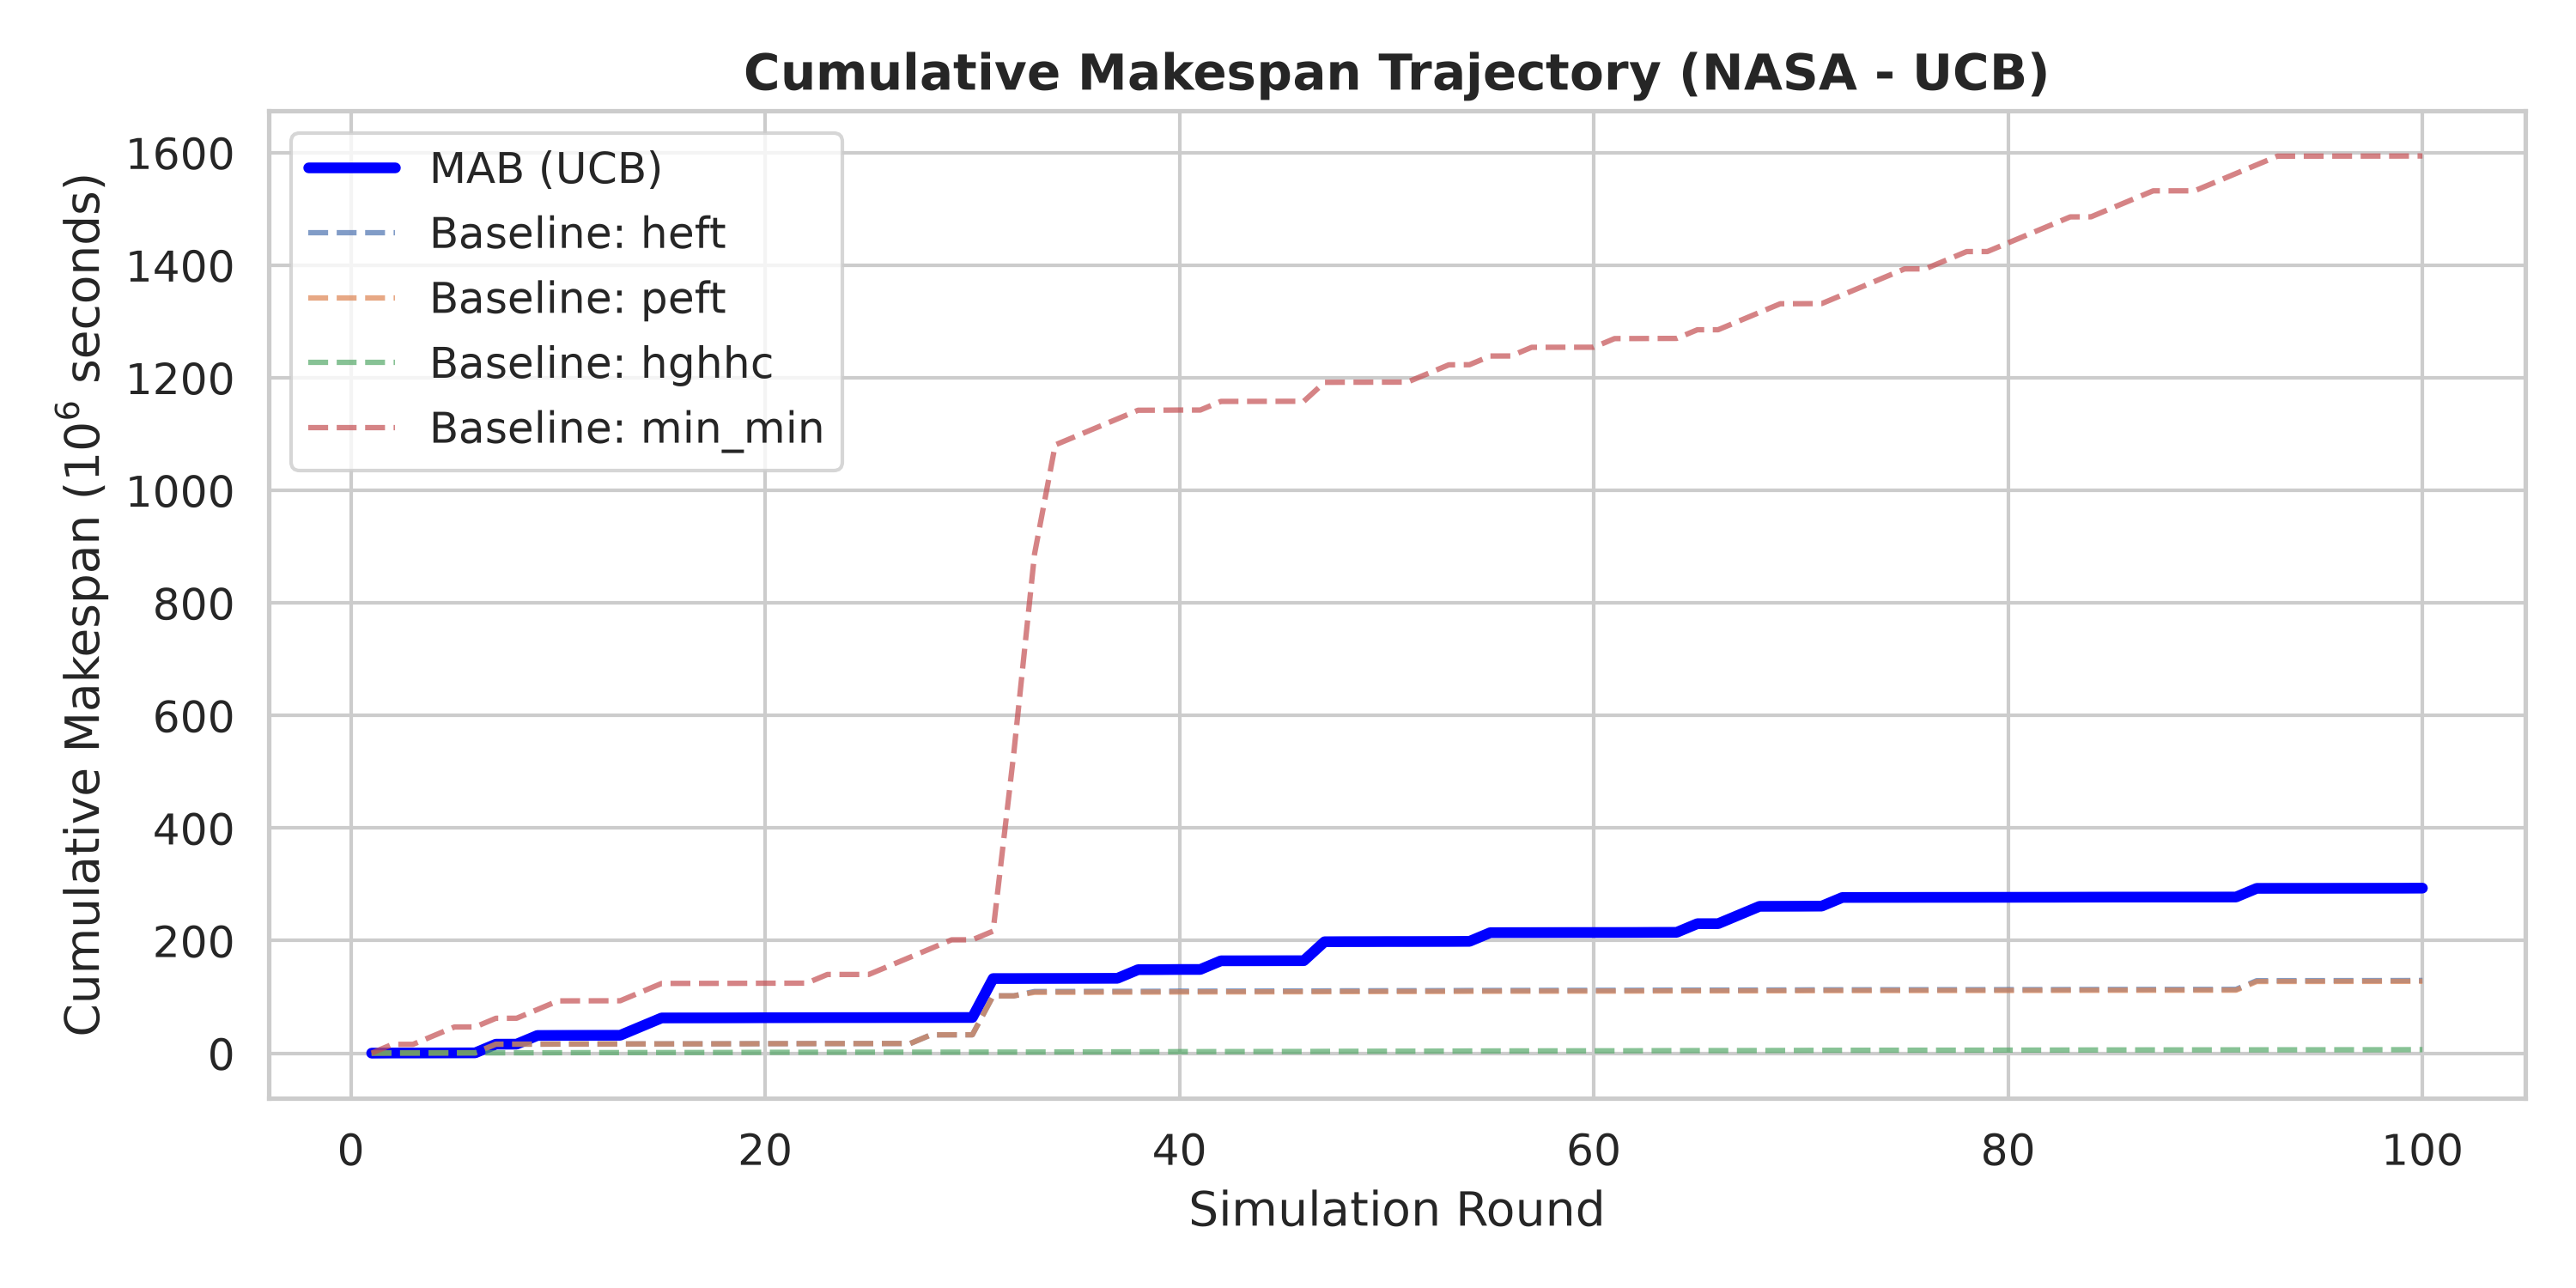
\includegraphics[width=\textwidth]{nasa_ucb_cumulative_makespan.png}
        \caption{NASA -- UCB}
        \label{fig:makespan_nasa_ucb}
    \end{subfigure}
    \hfill
    \begin{subfigure}[b]{0.48\textwidth}
        \centering
        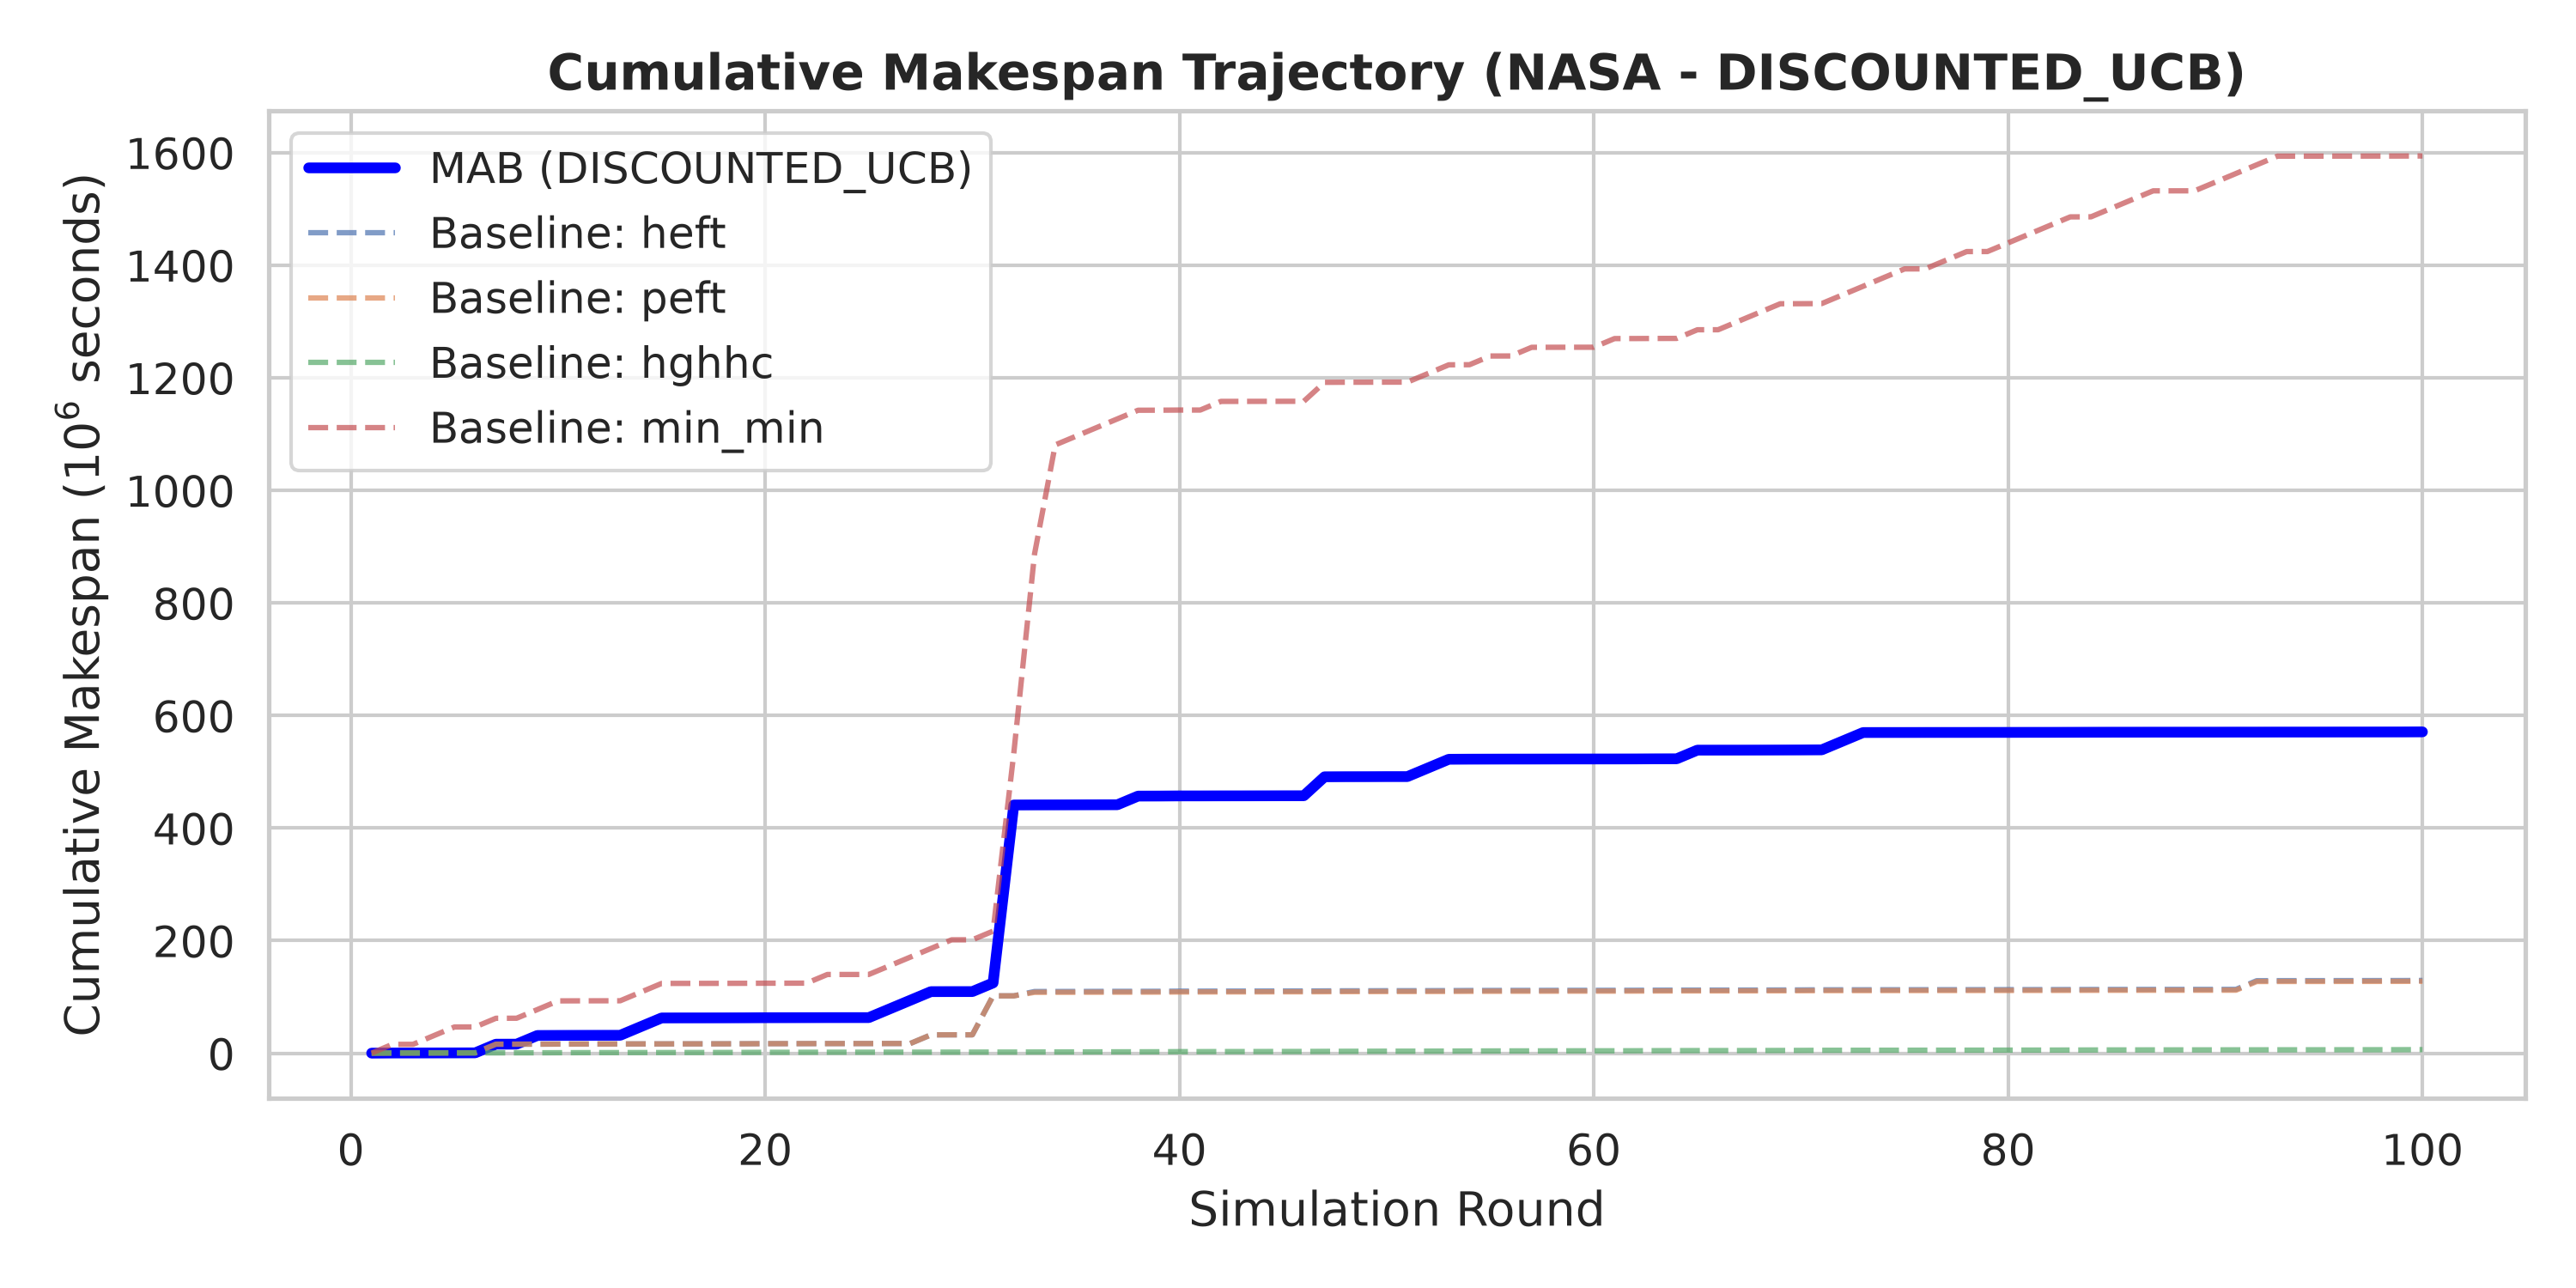
\includegraphics[width=\textwidth]{nasa_discounted_ucb_cumulative_makespan.png}
        \caption{NASA -- Discounted UCB}
        \label{fig:makespan_nasa_discounted}
    \end{subfigure}
    \vskip\baselineskip
    \begin{subfigure}[b]{0.48\textwidth}
        \centering
        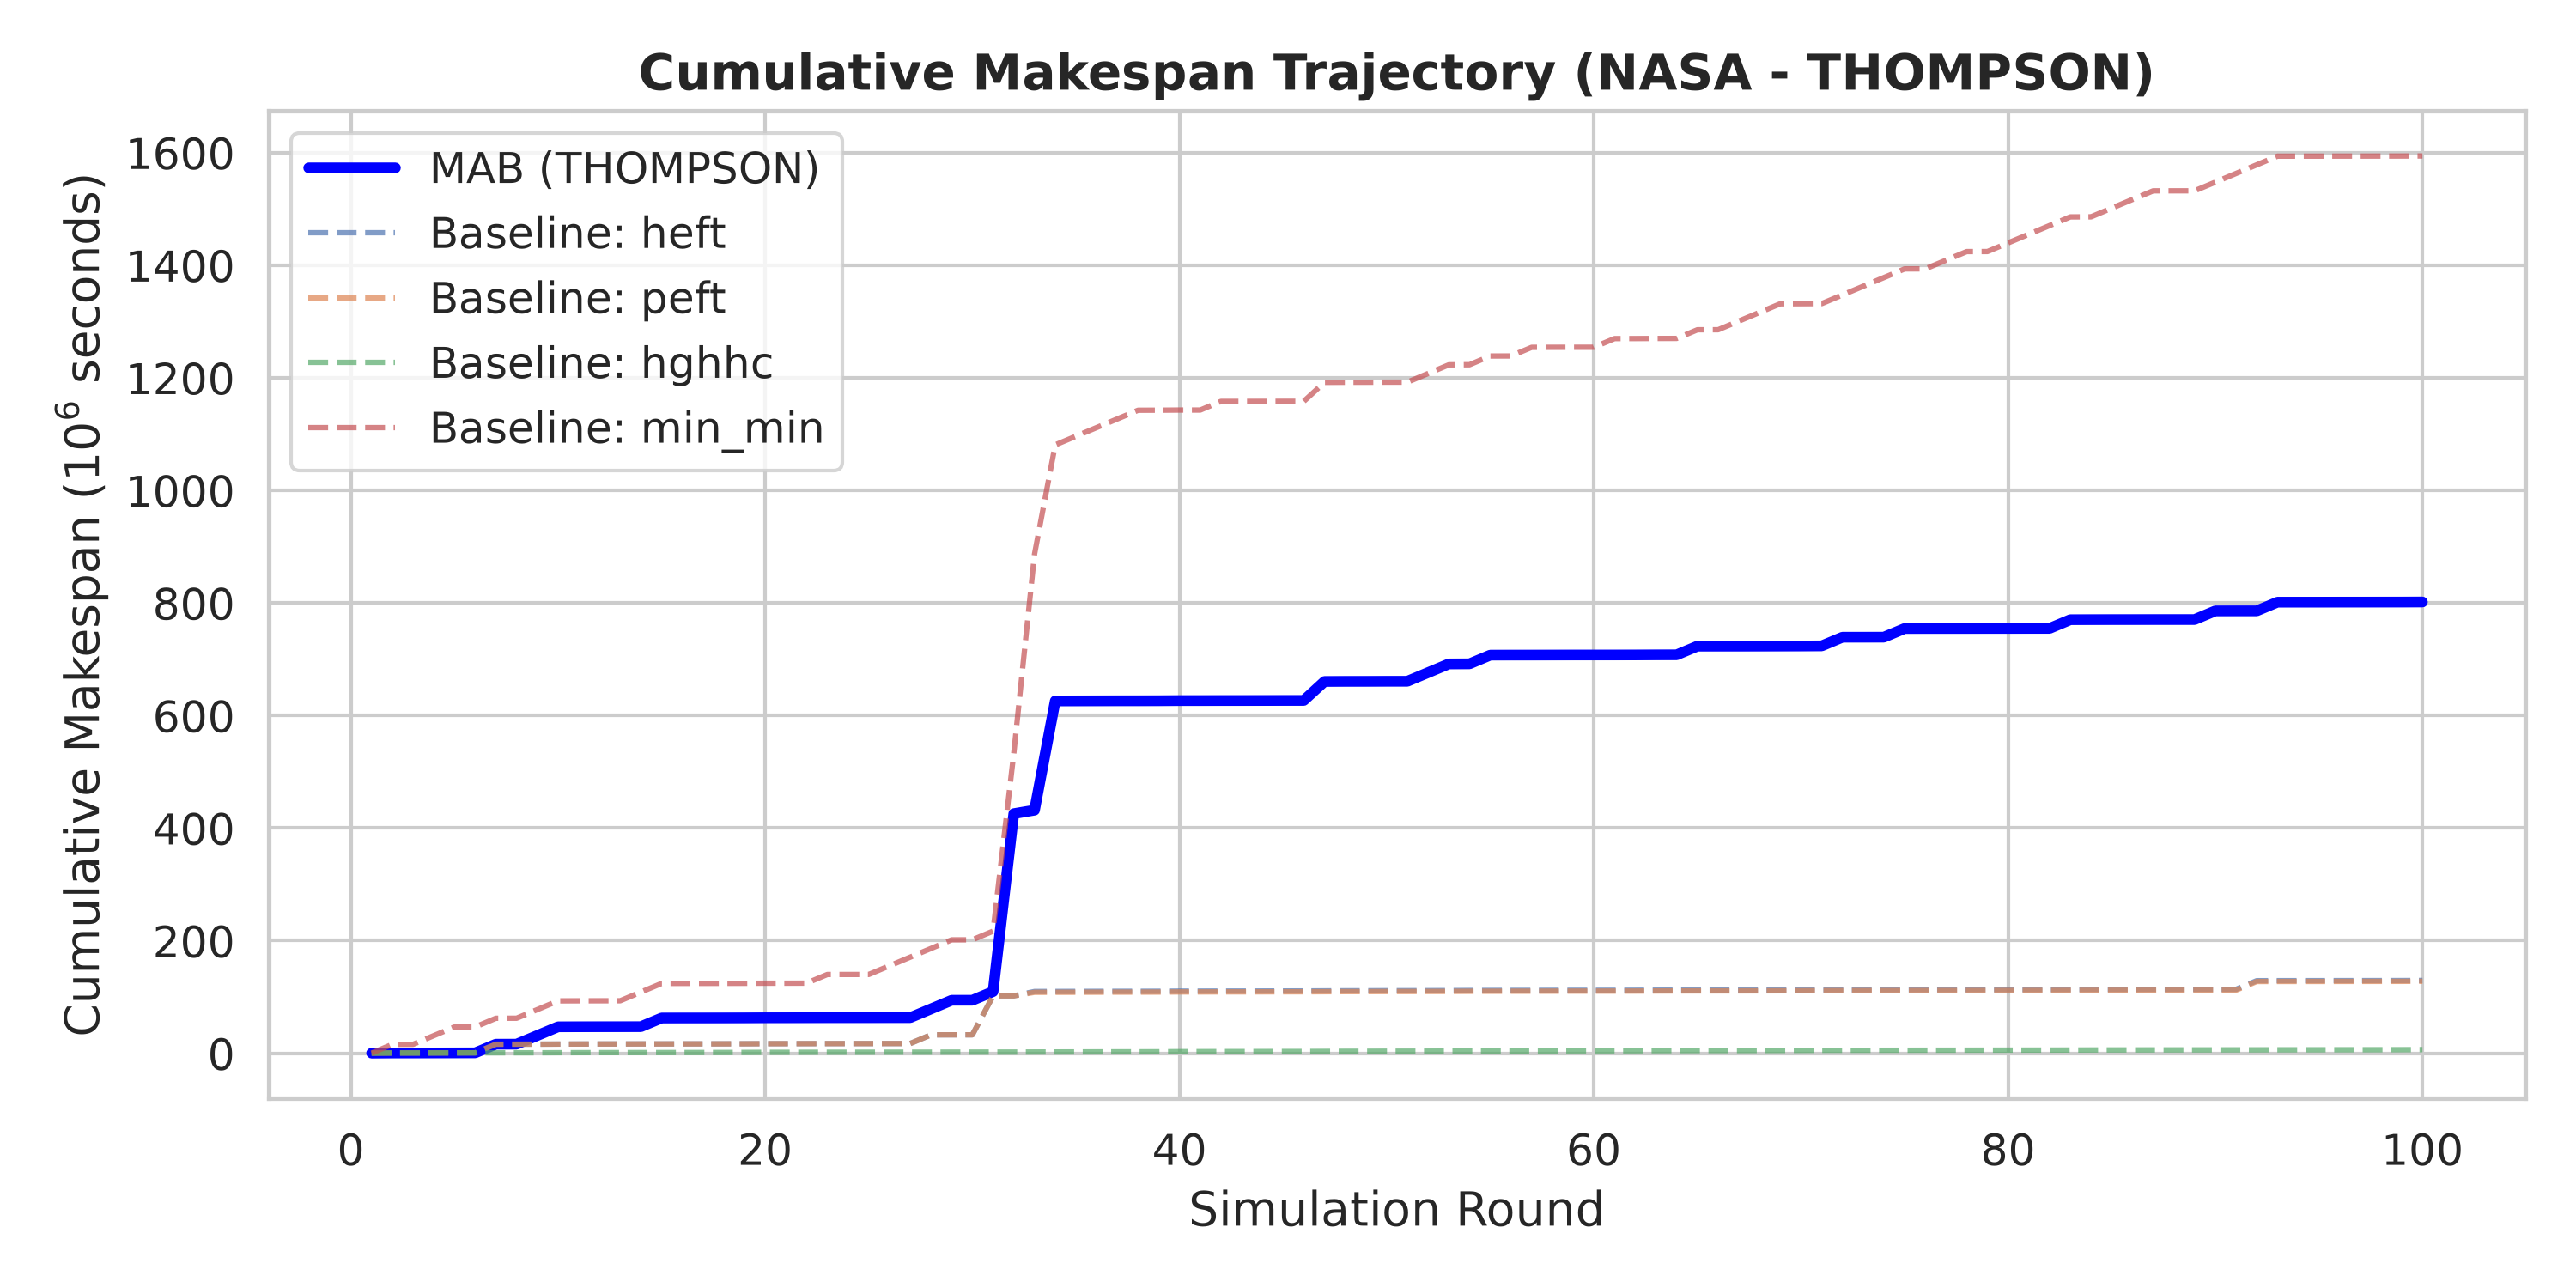
\includegraphics[width=\textwidth]{nasa_thompson_cumulative_makespan.png}
        \caption{NASA -- Thompson Sampling}
        \label{fig:makespan_nasa_thompson}
    \end{subfigure}
    \hfill
    \begin{subfigure}[b]{0.48\textwidth}
        \centering
        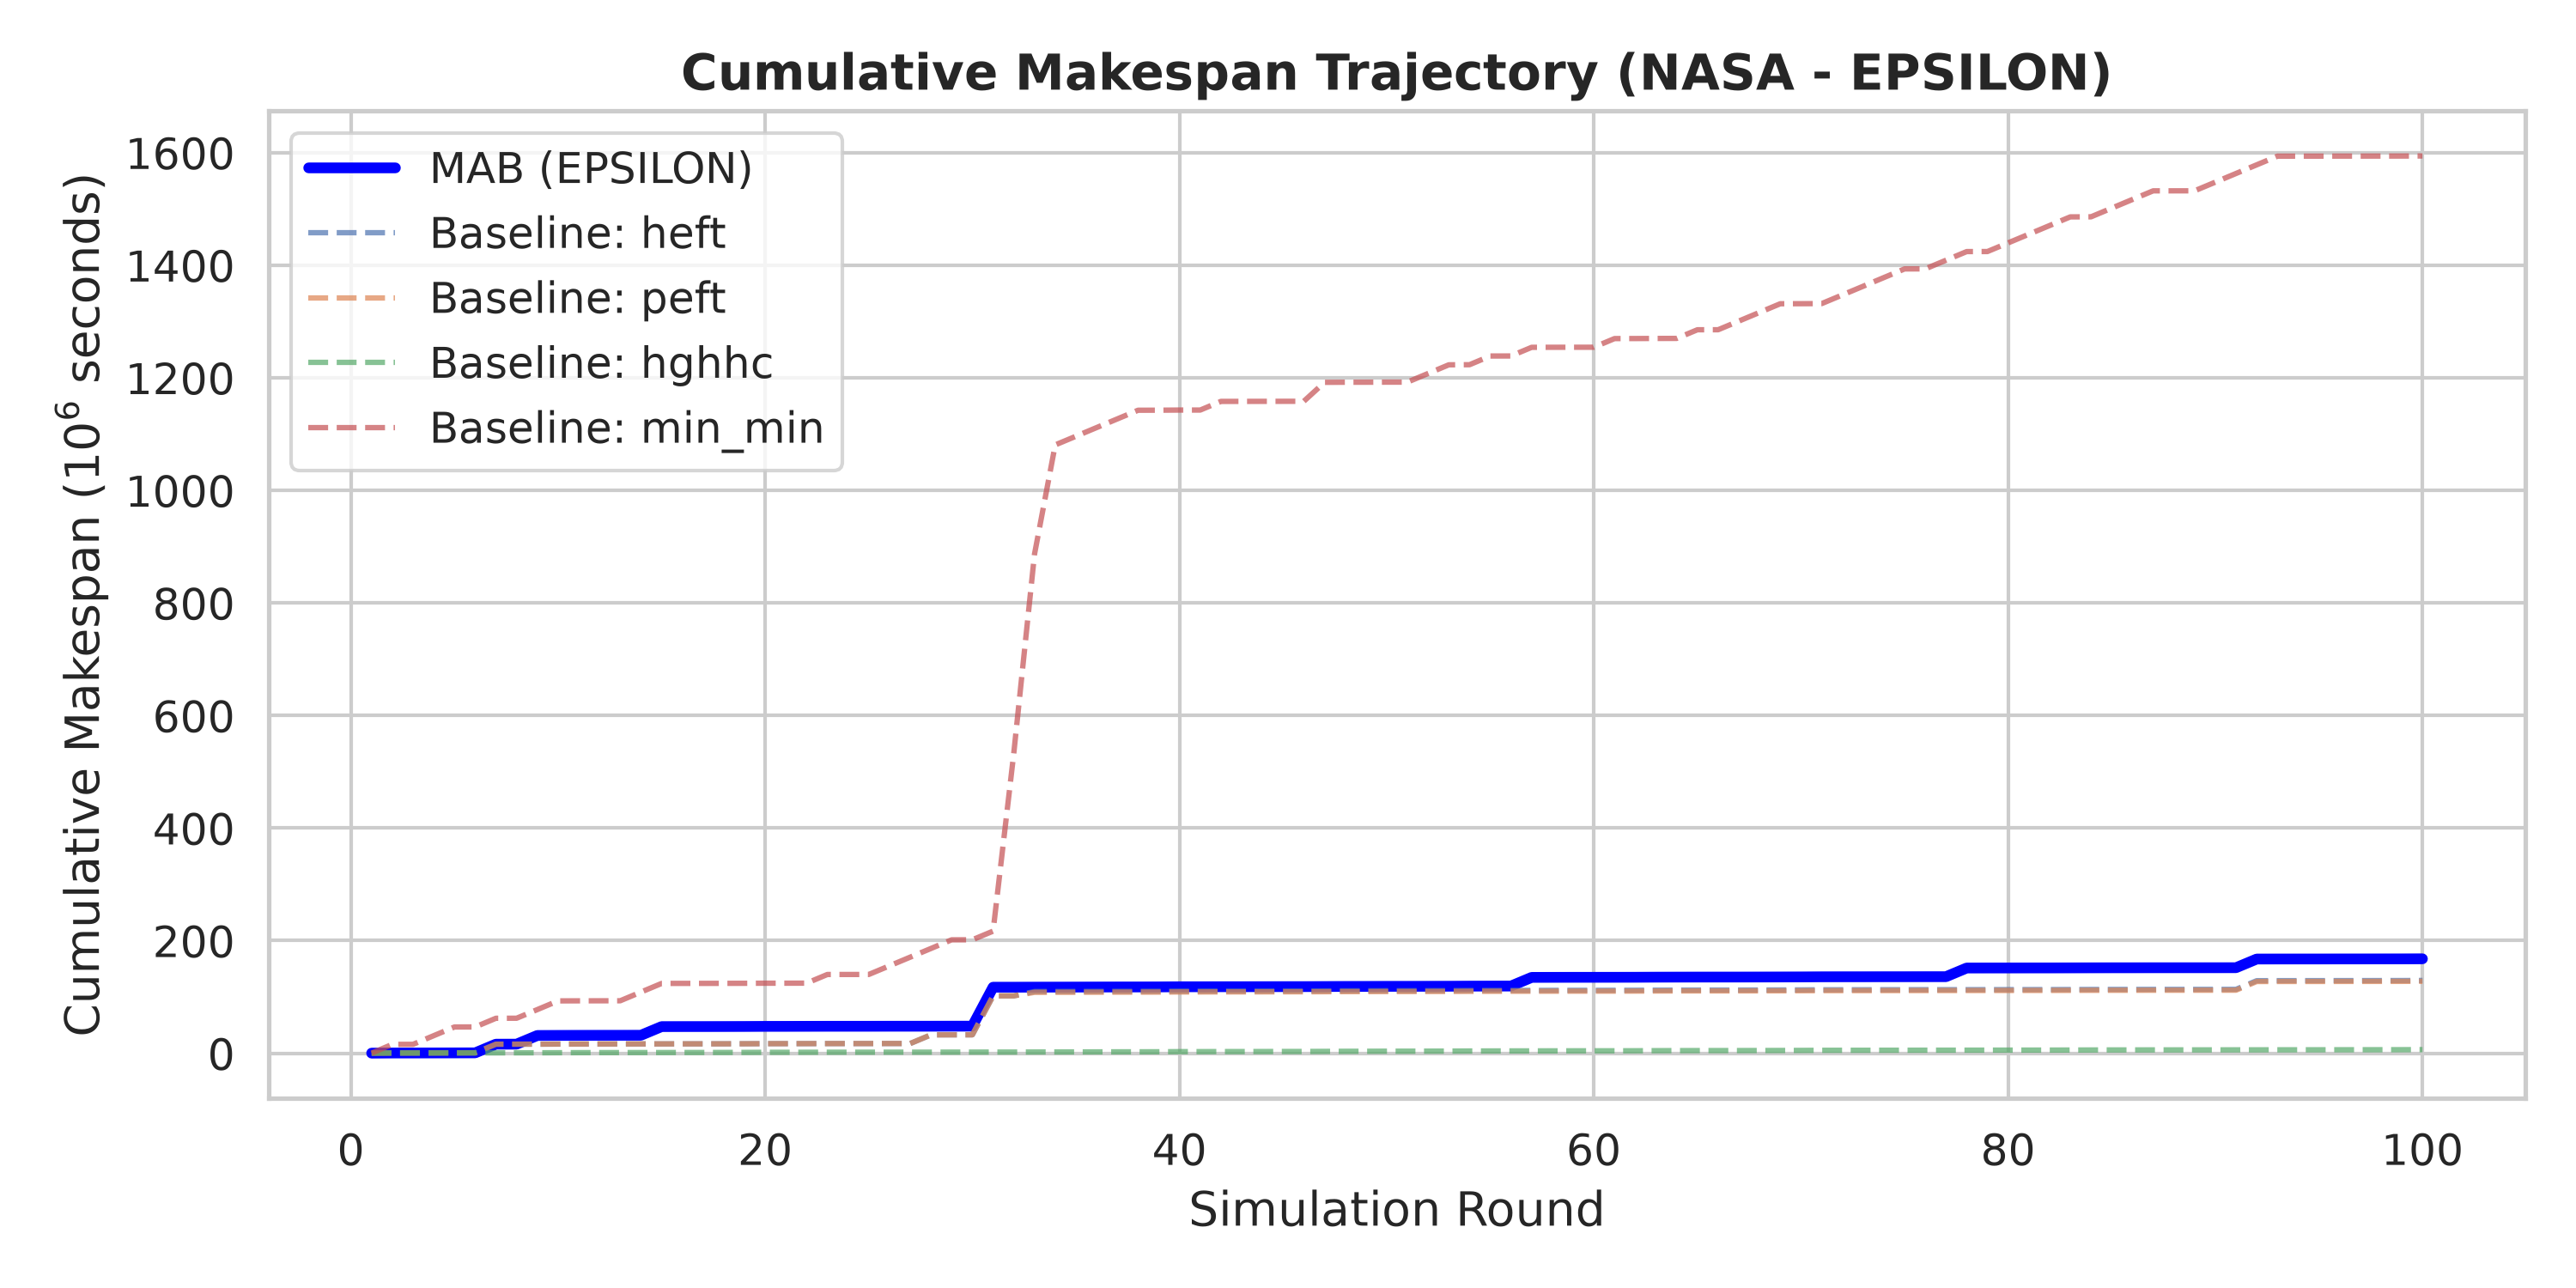
\includegraphics[width=\textwidth]{nasa_epsilon_cumulative_makespan.png}
        \caption{NASA -- $\epsilon$-Greedy}
        \label{fig:makespan_nasa_epsilon}
    \end{subfigure}
    \caption{Cumulative makespan trajectories across MAB variants on the NASA Ames workload.}
    \label{fig:makespan_nasa_all}
\end{figure}

The primary empirical insights include:
\begin{itemize}
    \item \textbf{Mitigation of Baseline Degradation:} Static \texttt{min\_min} exhibits severe performance degradation on NASA Ames (Figures~\ref{fig:makespan_nasa_ucb}--\ref{fig:makespan_nasa_epsilon}), accumulating over $1.6 \times 10^9$ seconds in makespan by round 100 due to severe task queueing. All MAB controllers avoid this failure mode by moving away from \texttt{min\_min} as early into the batch as possible.
    \item \textbf{Performance Superiority on HPC2N:} On HPC2N (Figure~\ref{fig:makespan_hpc2n_all}), standard UCB, Discounted UCB, Thompson Sampling, and $\epsilon$-Greedy all show a $59.5\%$--$71.4\%$ improvement over \texttt{min\_min} and constantly outperforms the static list schedulers.
    \item \textbf{Exploration Penalty under Thompson Sampling:} On NASA Ames (Figure~\ref{fig:makespan_nasa_thompson}), Thompson Sampling accumulates $8.0 \times 10^8$ seconds makespan, whereas $\epsilon$-Greedy (Figure~\ref{fig:makespan_nasa_epsilon}) terminates at $1.7 \times 10^8$ seconds, which shows that posterior sampling can lead to unnecessary exploration overhead in fairly predictable workloads.
\end{itemize}

% \subsubsection{Multi-Objective Radar Profile Analysis}
% Figures~\ref{fig:radar_hpc2n_all} and~\ref{fig:radar_nasa_all} compare normalized multi-objective trade-offs (Makespan, Cost, Carbon Footprint, and VM Utilization) on HPC2N and NASA Ames traces.

% \begin{figure}[htbp]
%     \centering
%     \begin{subfigure}[b]{0.48\textwidth}
%         \centering
%         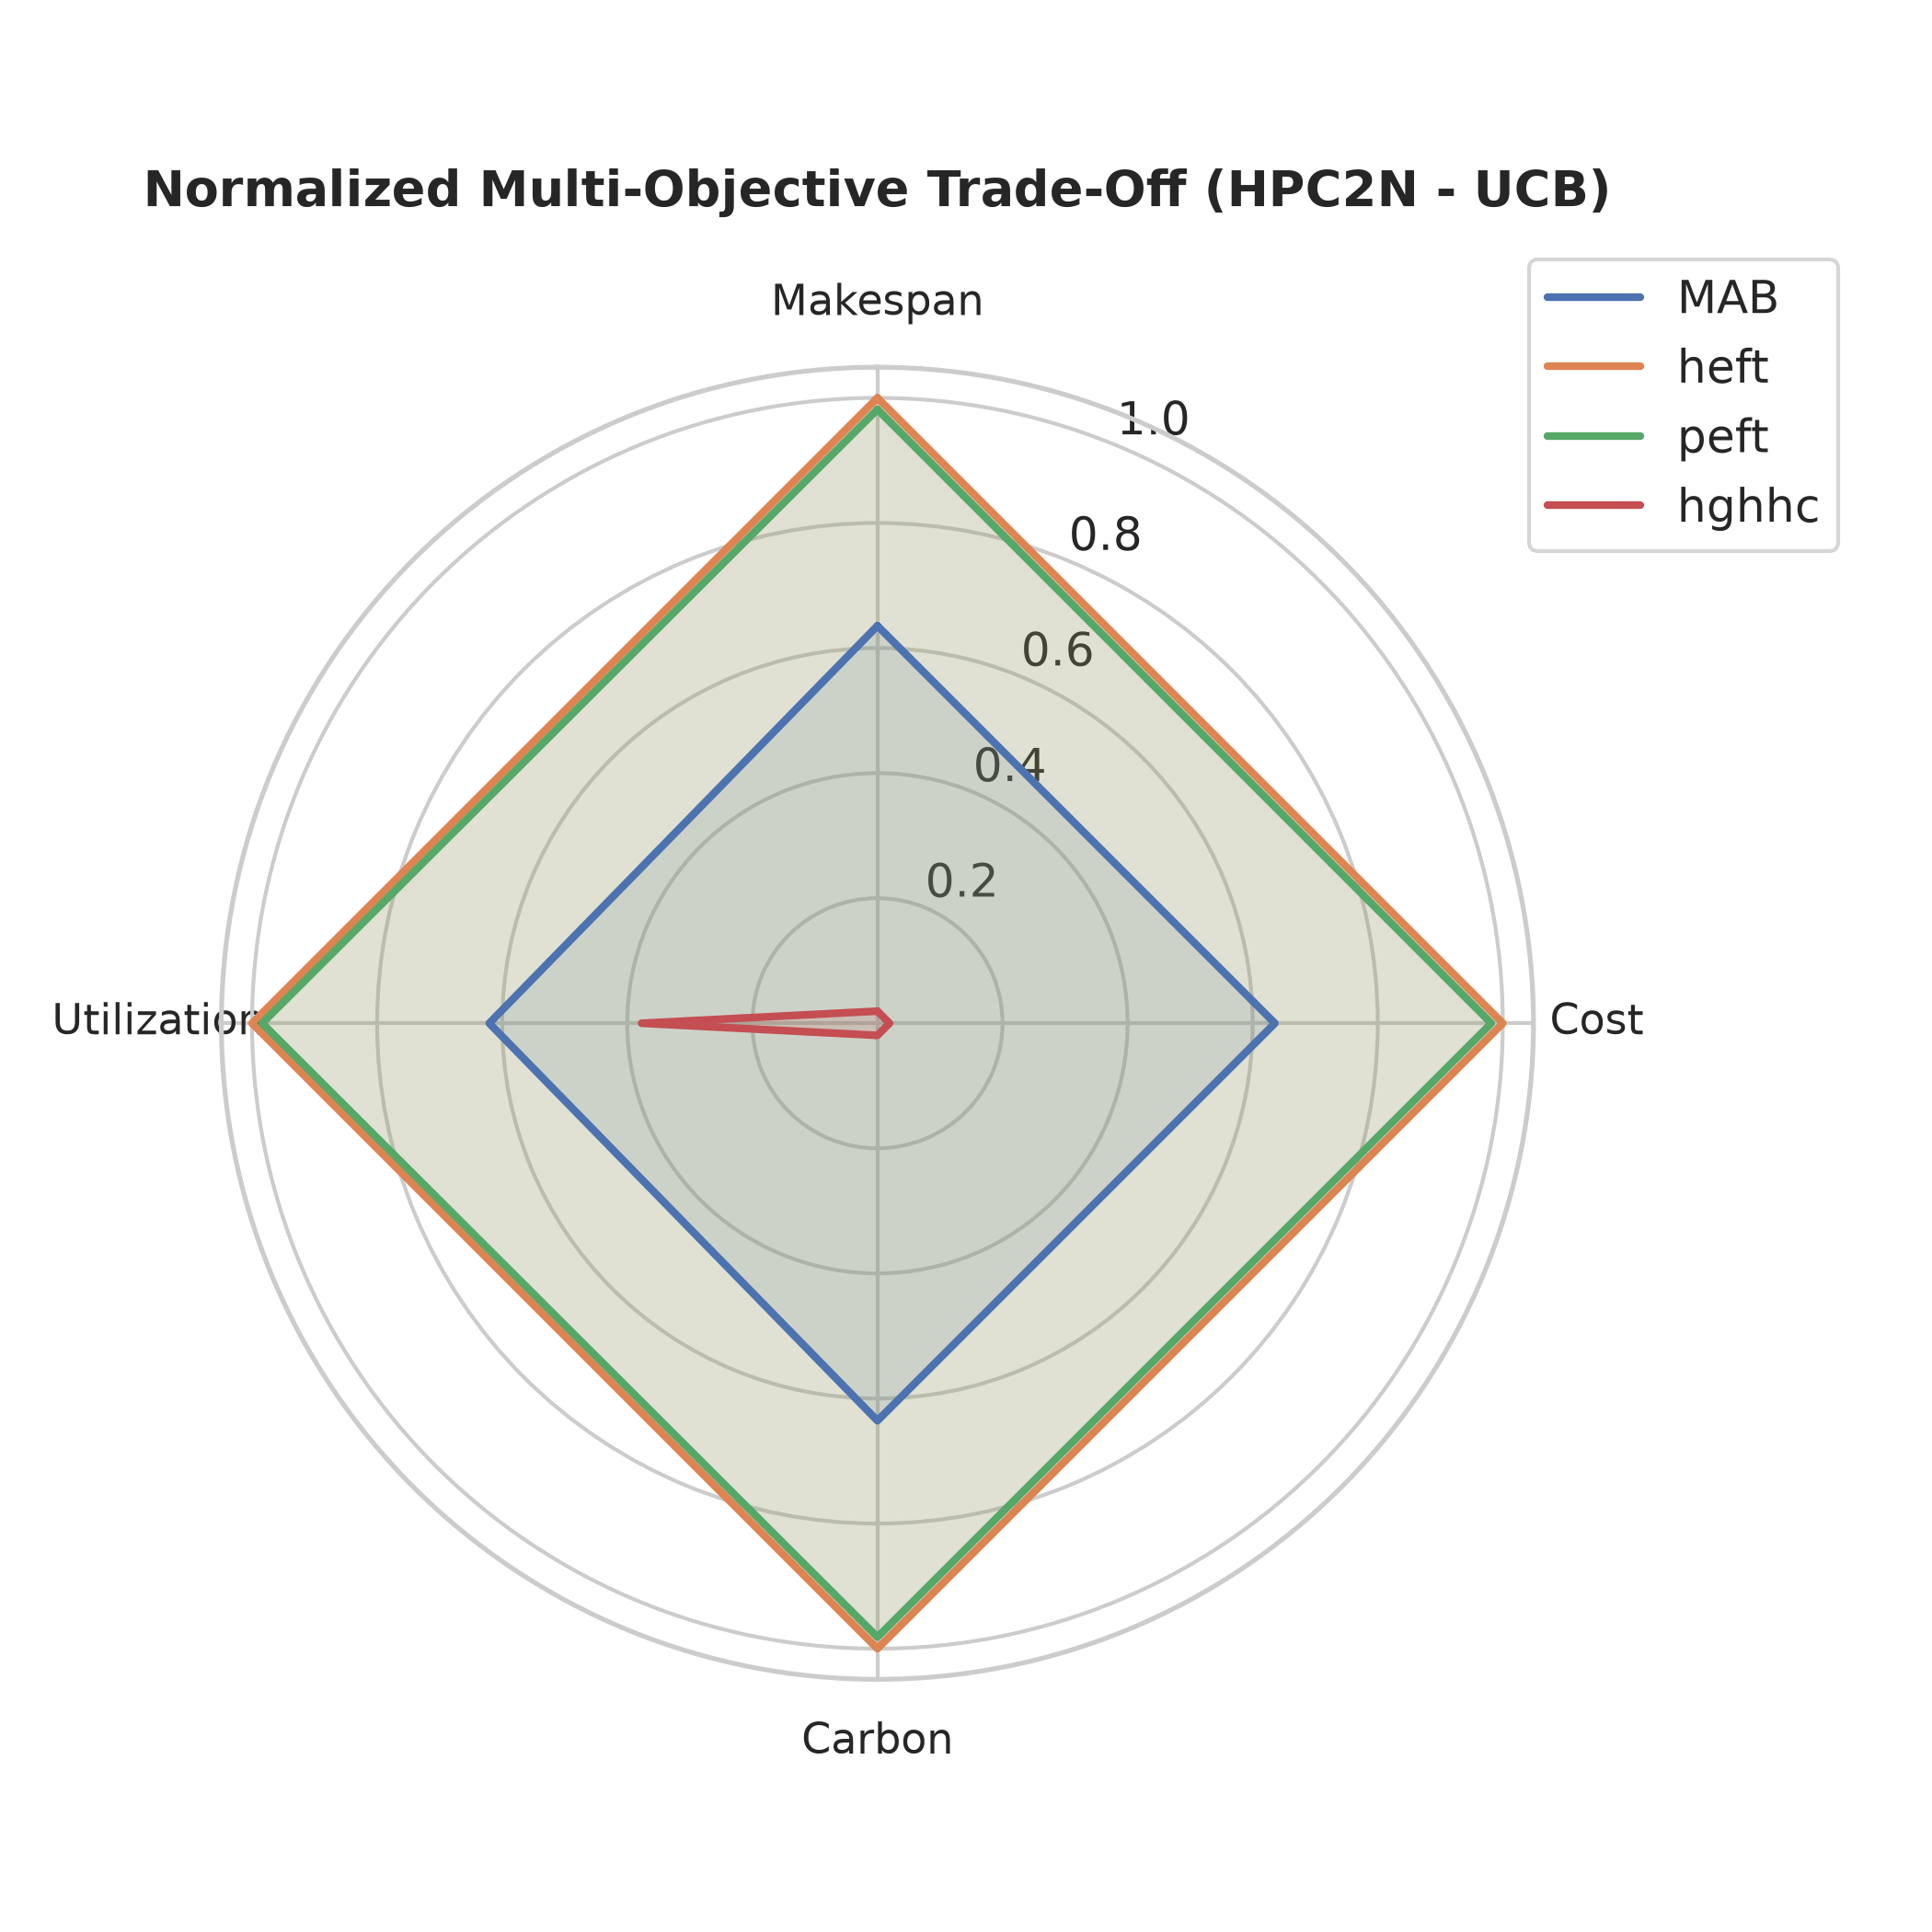
\includegraphics[width=\textwidth]{hpc2n_ucb_radar_multimetric.png}
%         \caption{HPC2N -- UCB}
%         \label{fig:radar_hpc2n_ucb}
%     \end{subfigure}
%     \hfill
%     \begin{subfigure}[b]{0.48\textwidth}
%         \centering
%         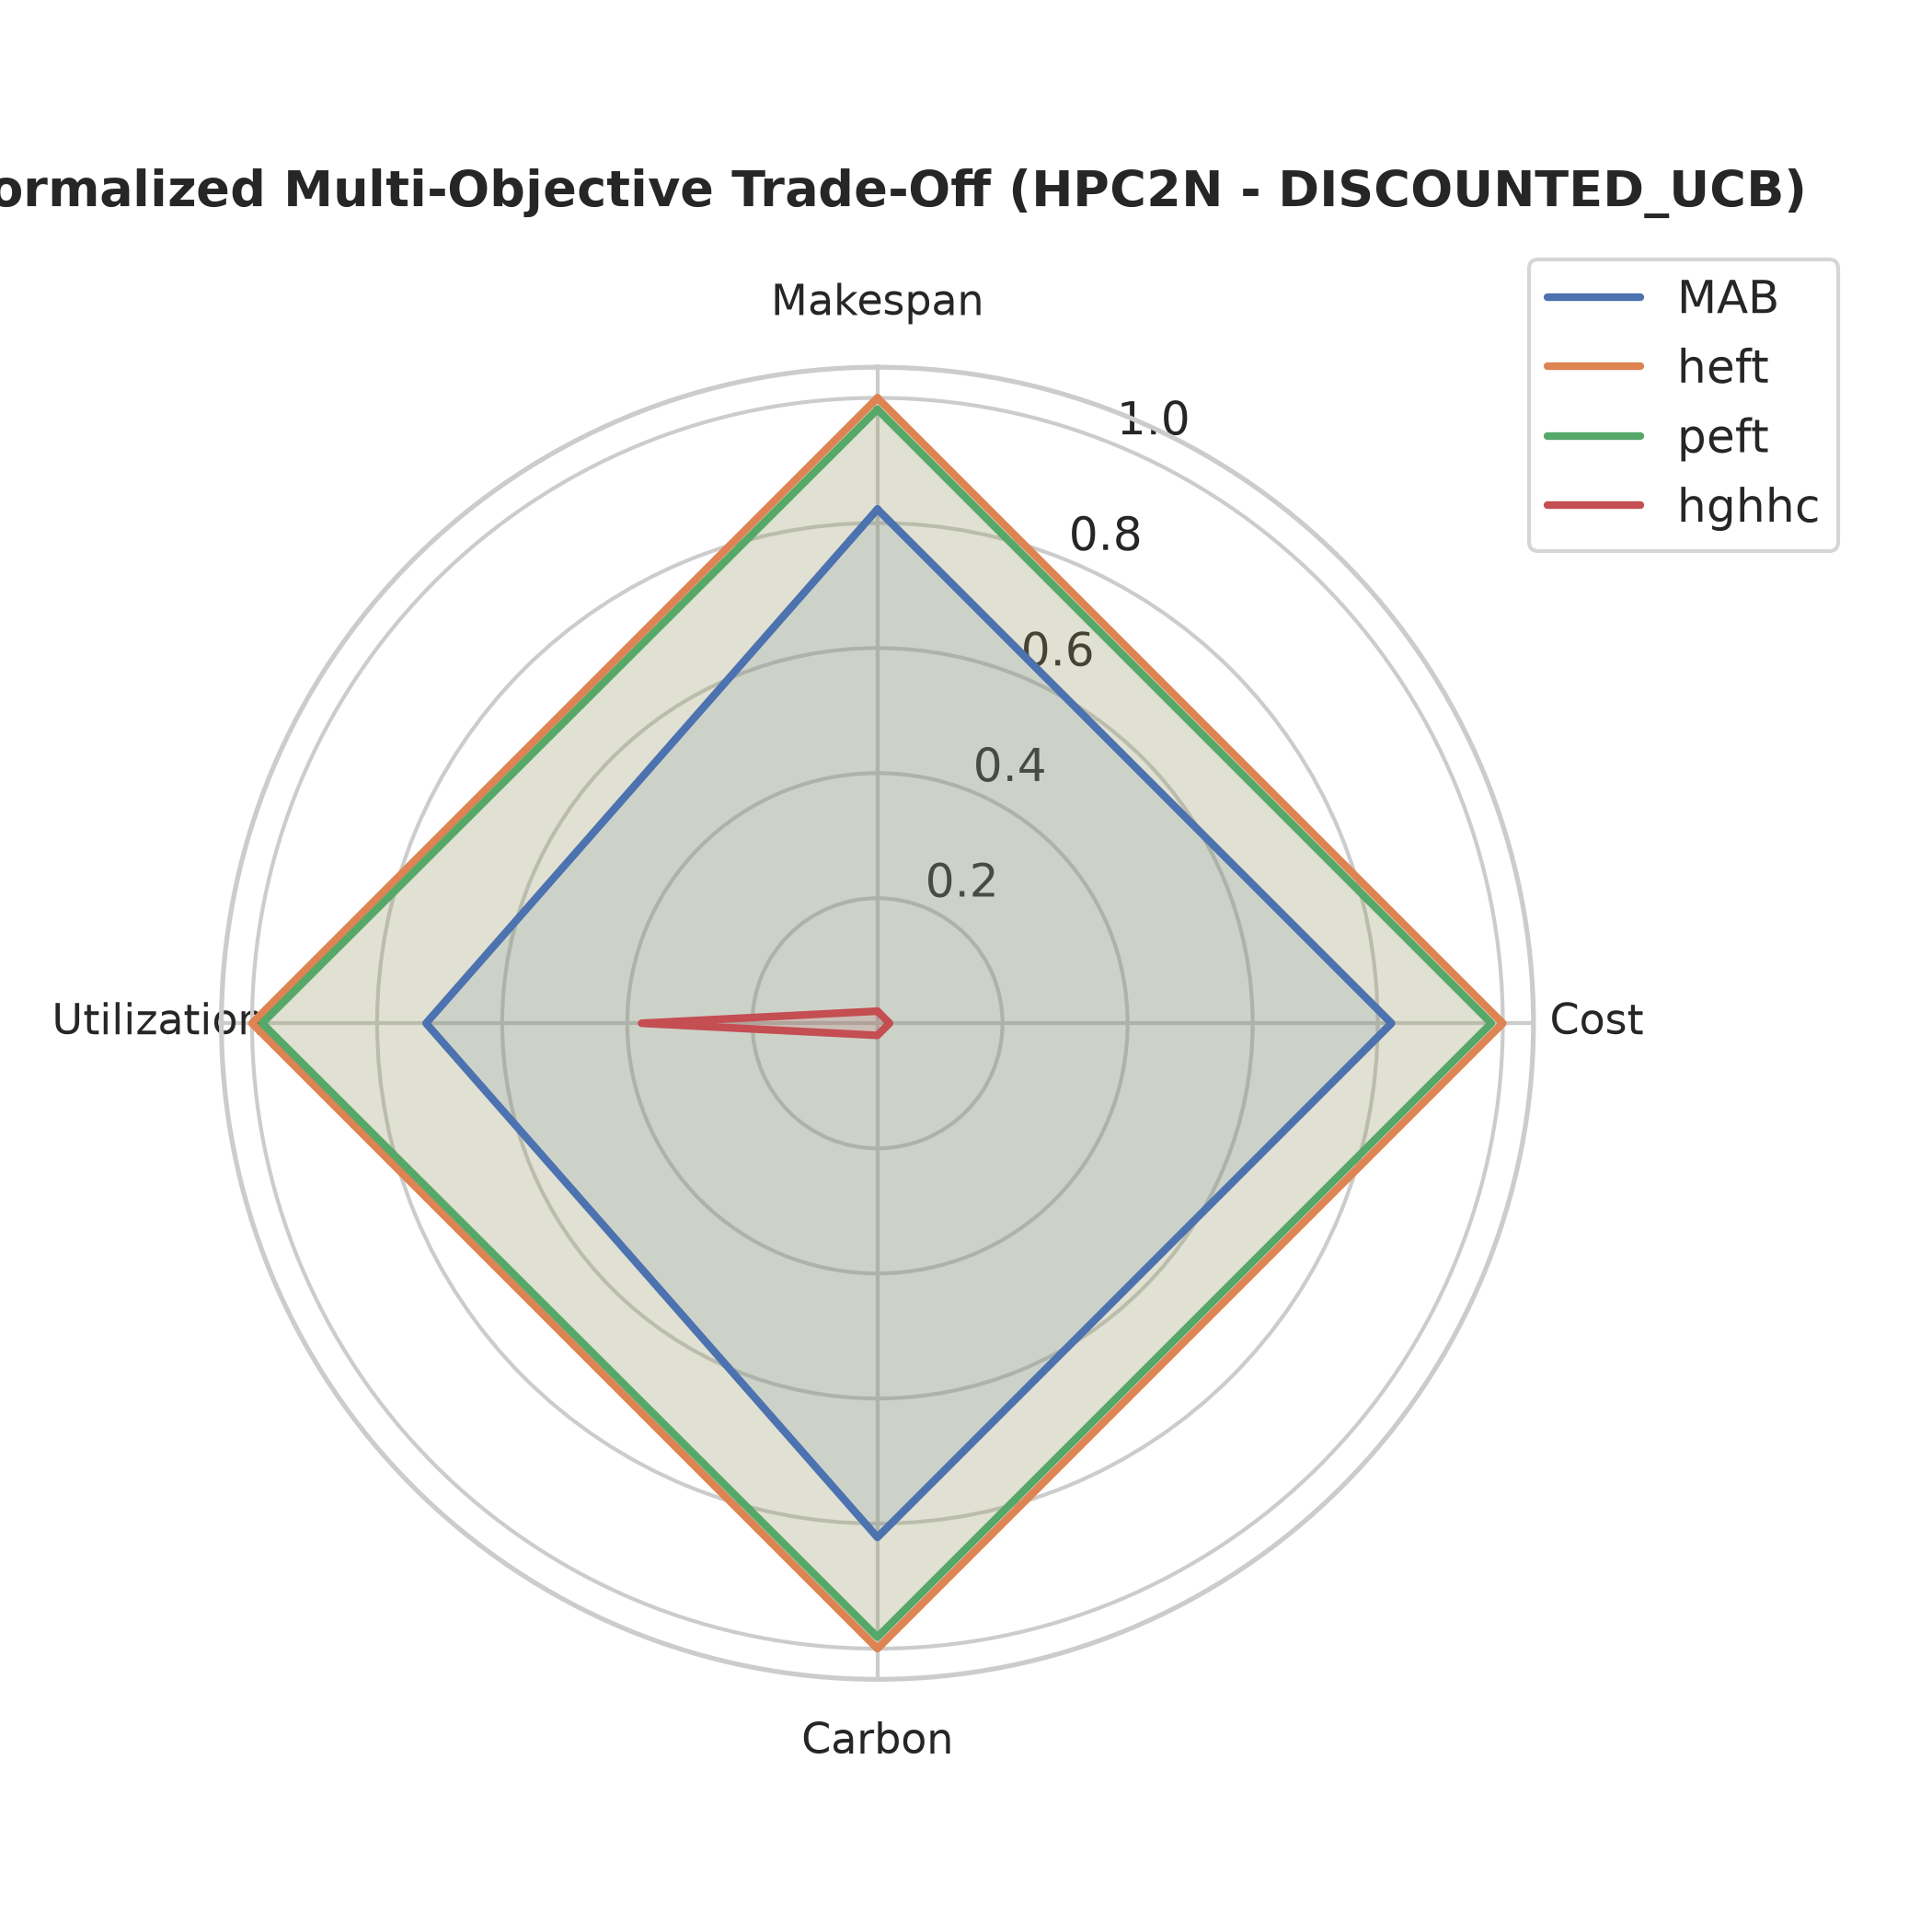
\includegraphics[width=\textwidth]{hpc2n_discounted_ucb_radar_multimetric.png}
%         \caption{HPC2N -- Discounted UCB}
%         \label{fig:radar_hpc2n_discounted}
%     \end{subfigure}
%     \vskip\baselineskip
%     \begin{subfigure}[b]{0.48\textwidth}
%         \centering
%         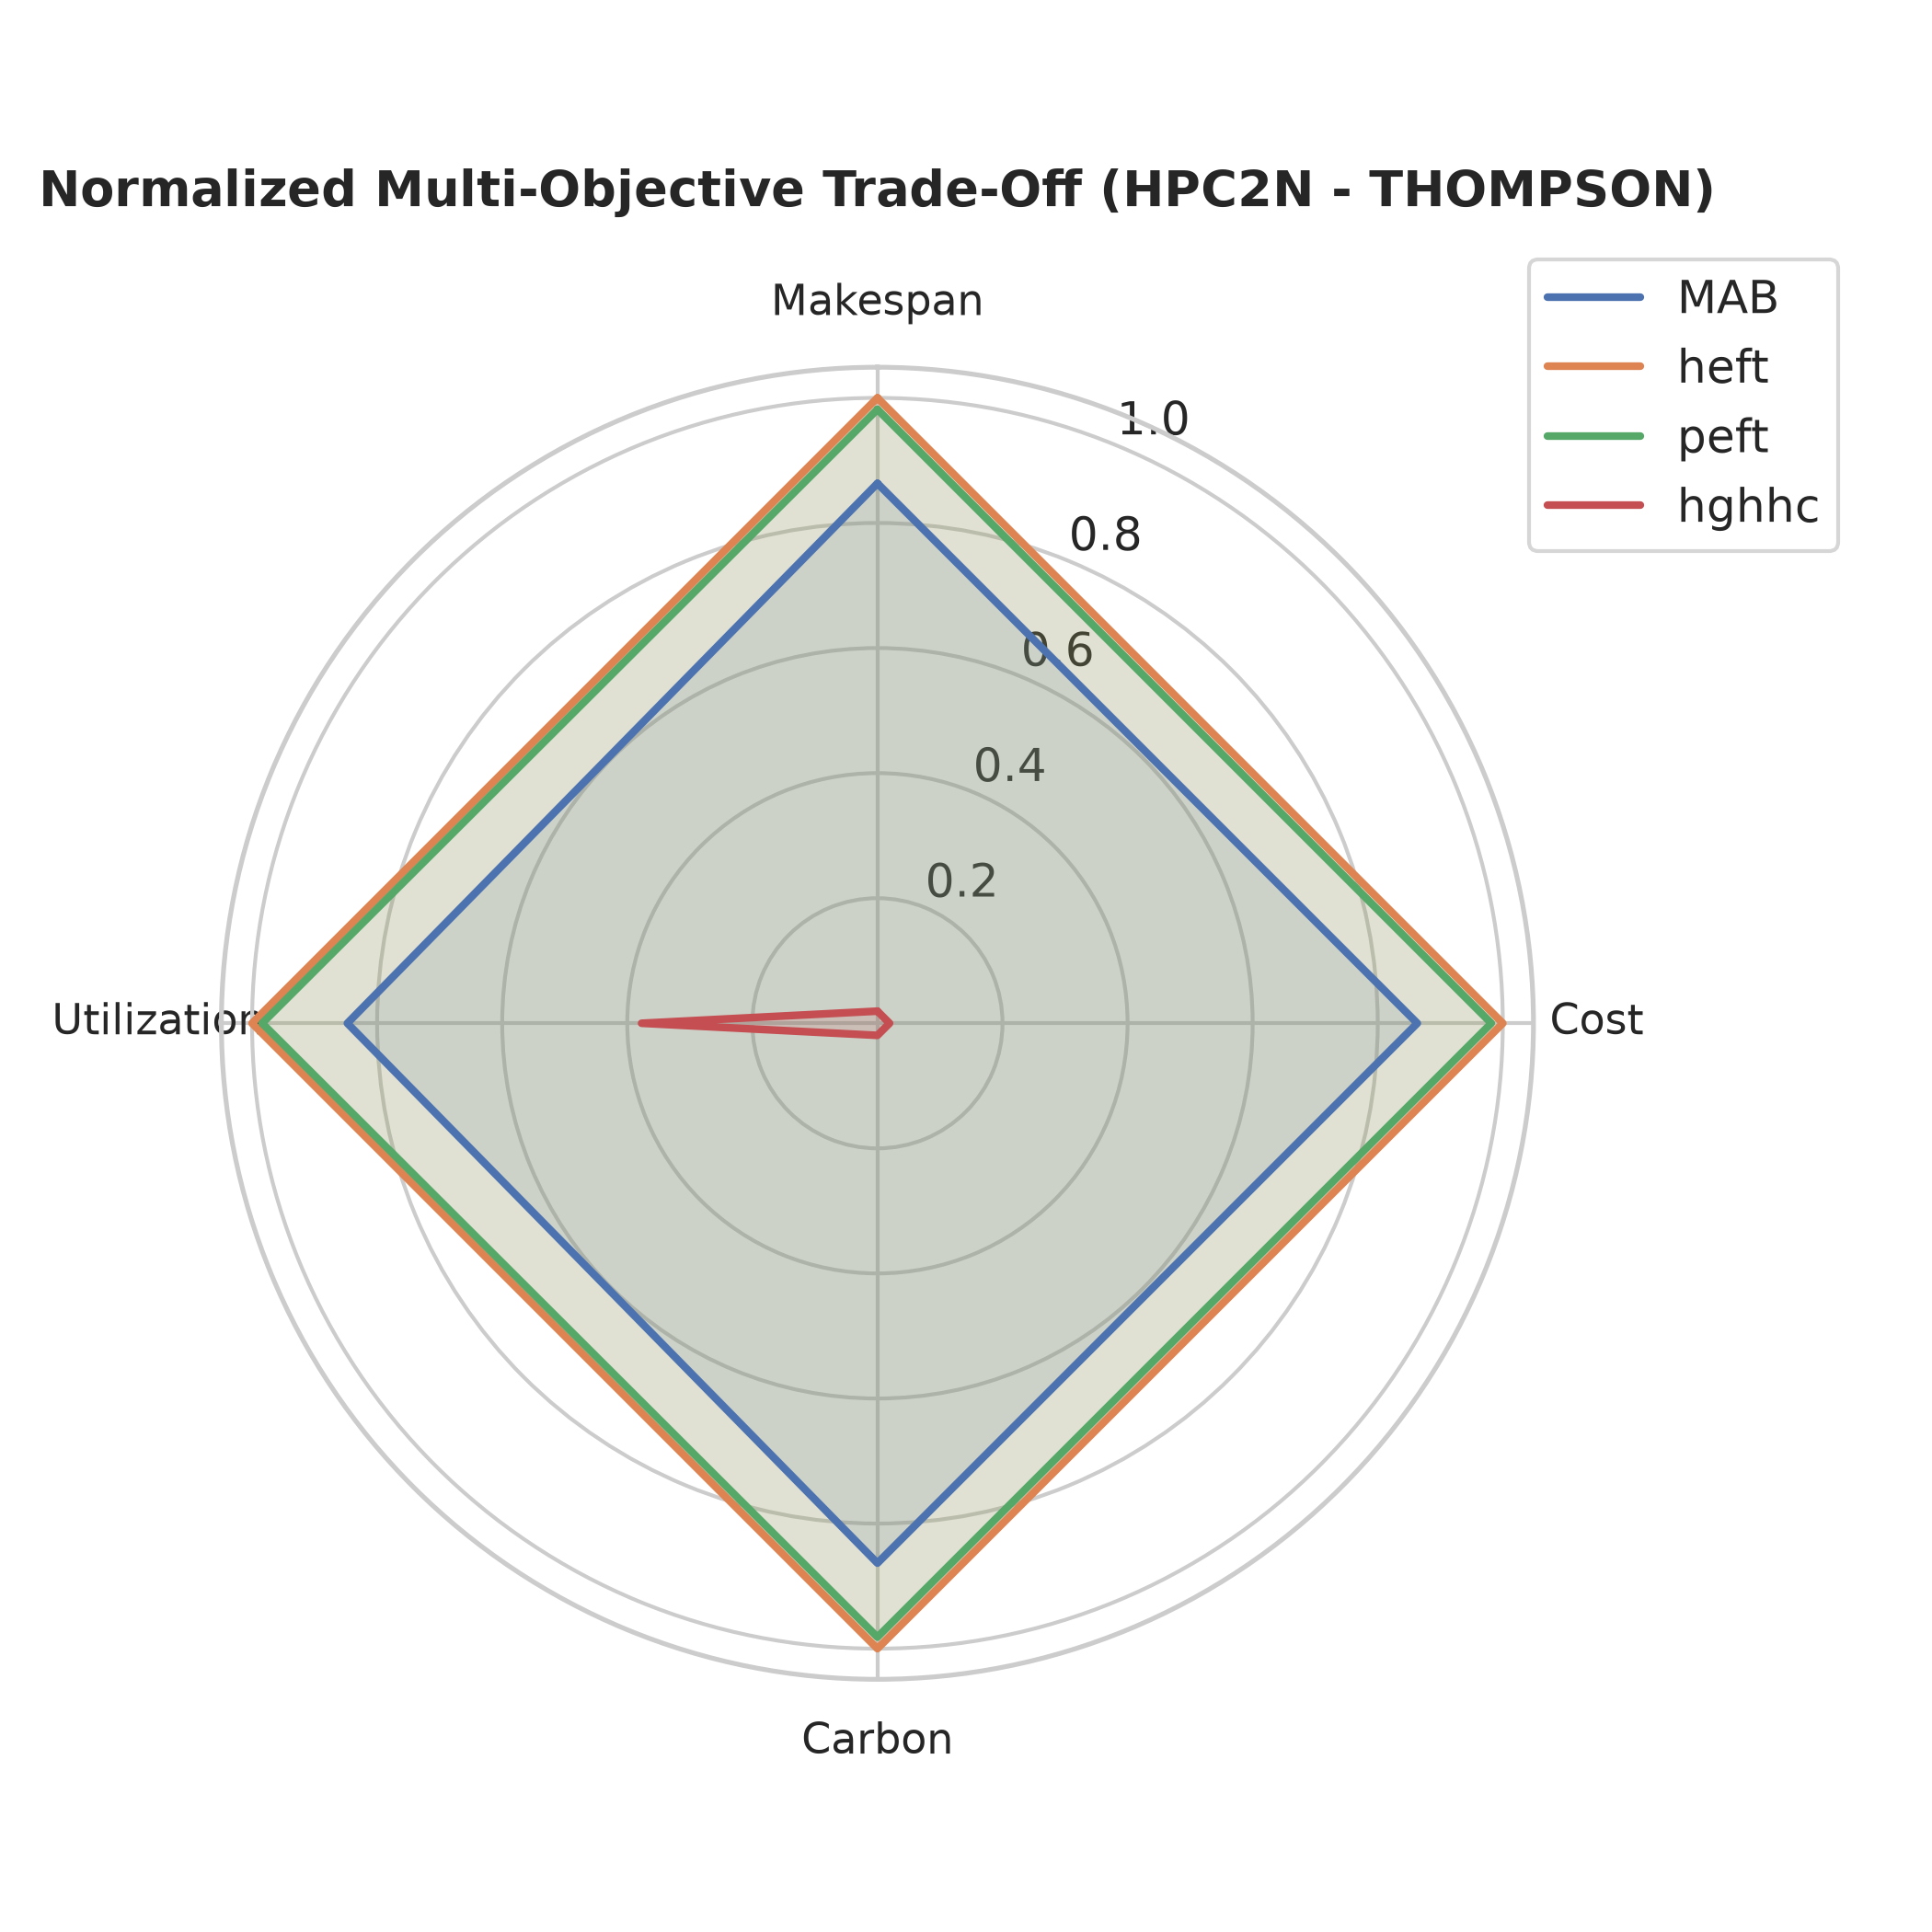
\includegraphics[width=\textwidth]{hpc2n_thompson_radar_multimetric.png}
%         \caption{HPC2N -- Thompson Sampling}
%         \label{fig:radar_hpc2n_thompson}
%     \end{subfigure}
%     \hfill
%     \begin{subfigure}[b]{0.48\textwidth}
%         \centering
%         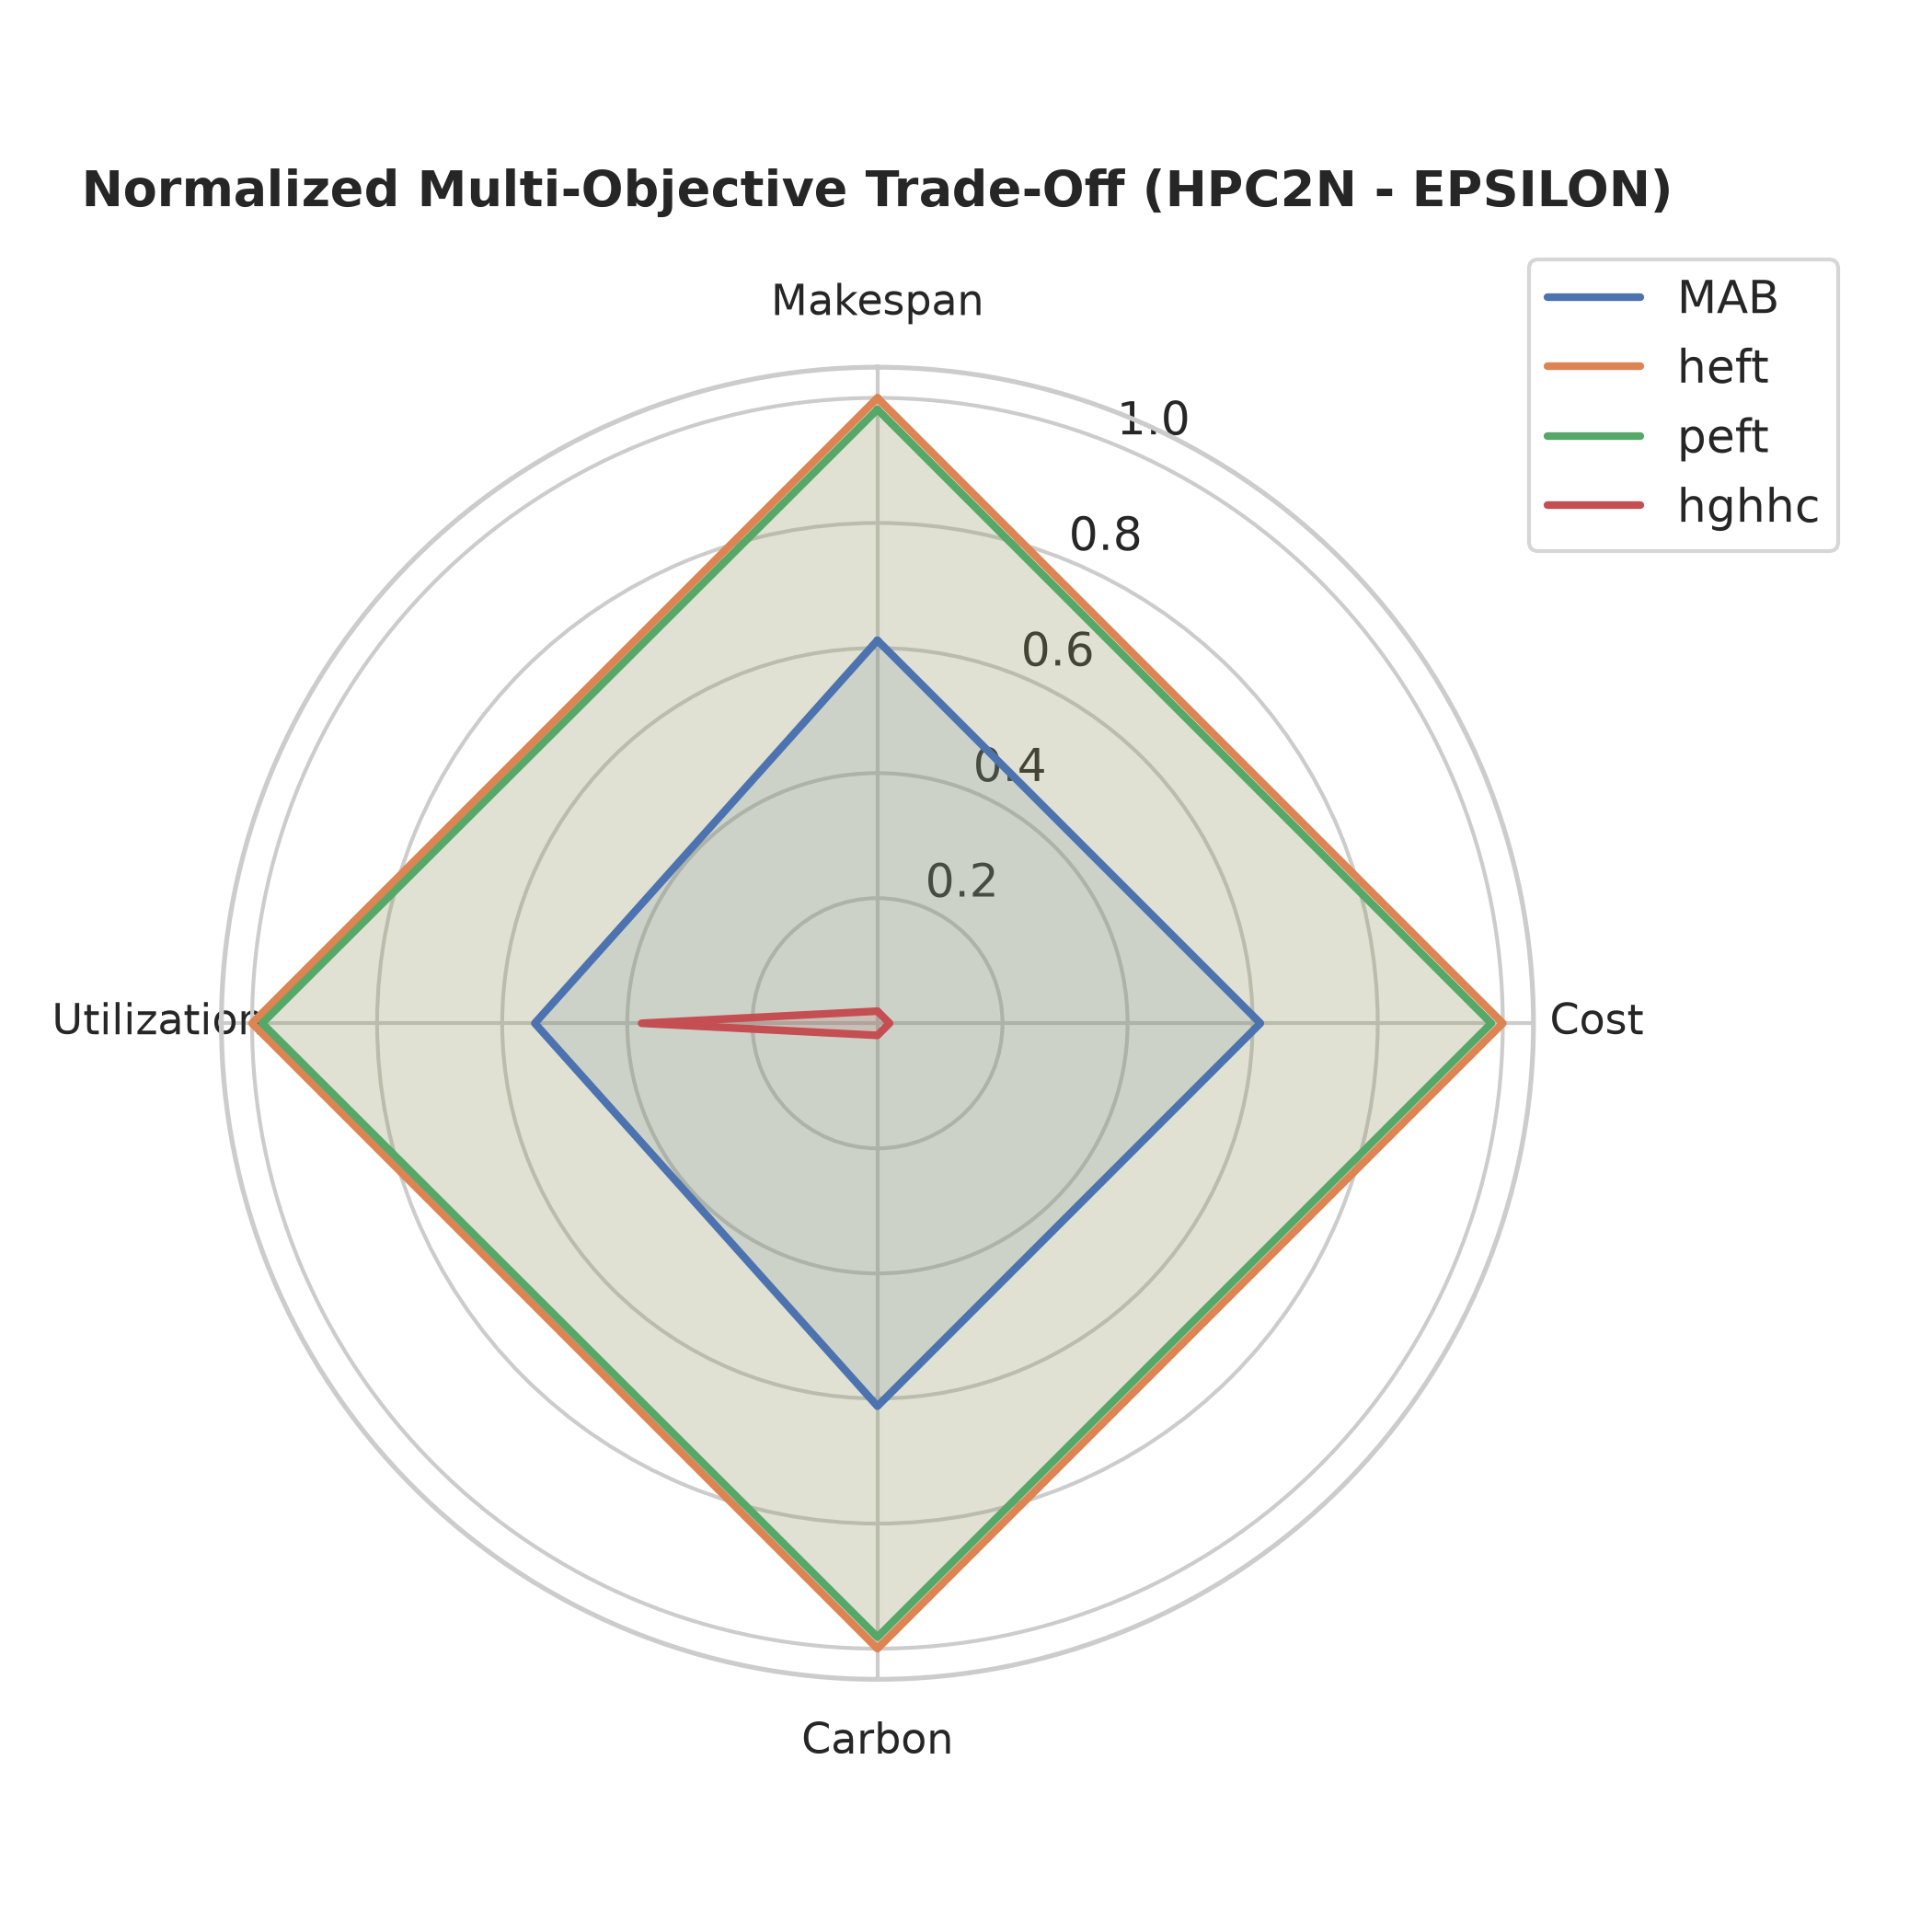
\includegraphics[width=\textwidth]{hpc2n_epsilon_radar_multimetric.png}
%         \caption{HPC2N -- $\epsilon$-Greedy}
%         \label{fig:radar_hpc2n_epsilon}
%     \end{subfigure}
%     \caption{Normalized multi-objective performance trade-offs on the HPC2N trace.}
%     \label{fig:radar_hpc2n_all}
% \end{figure}

% \begin{figure}[htbp]
%     \centering
%     \begin{subfigure}[b]{0.48\textwidth}
%         \centering
%         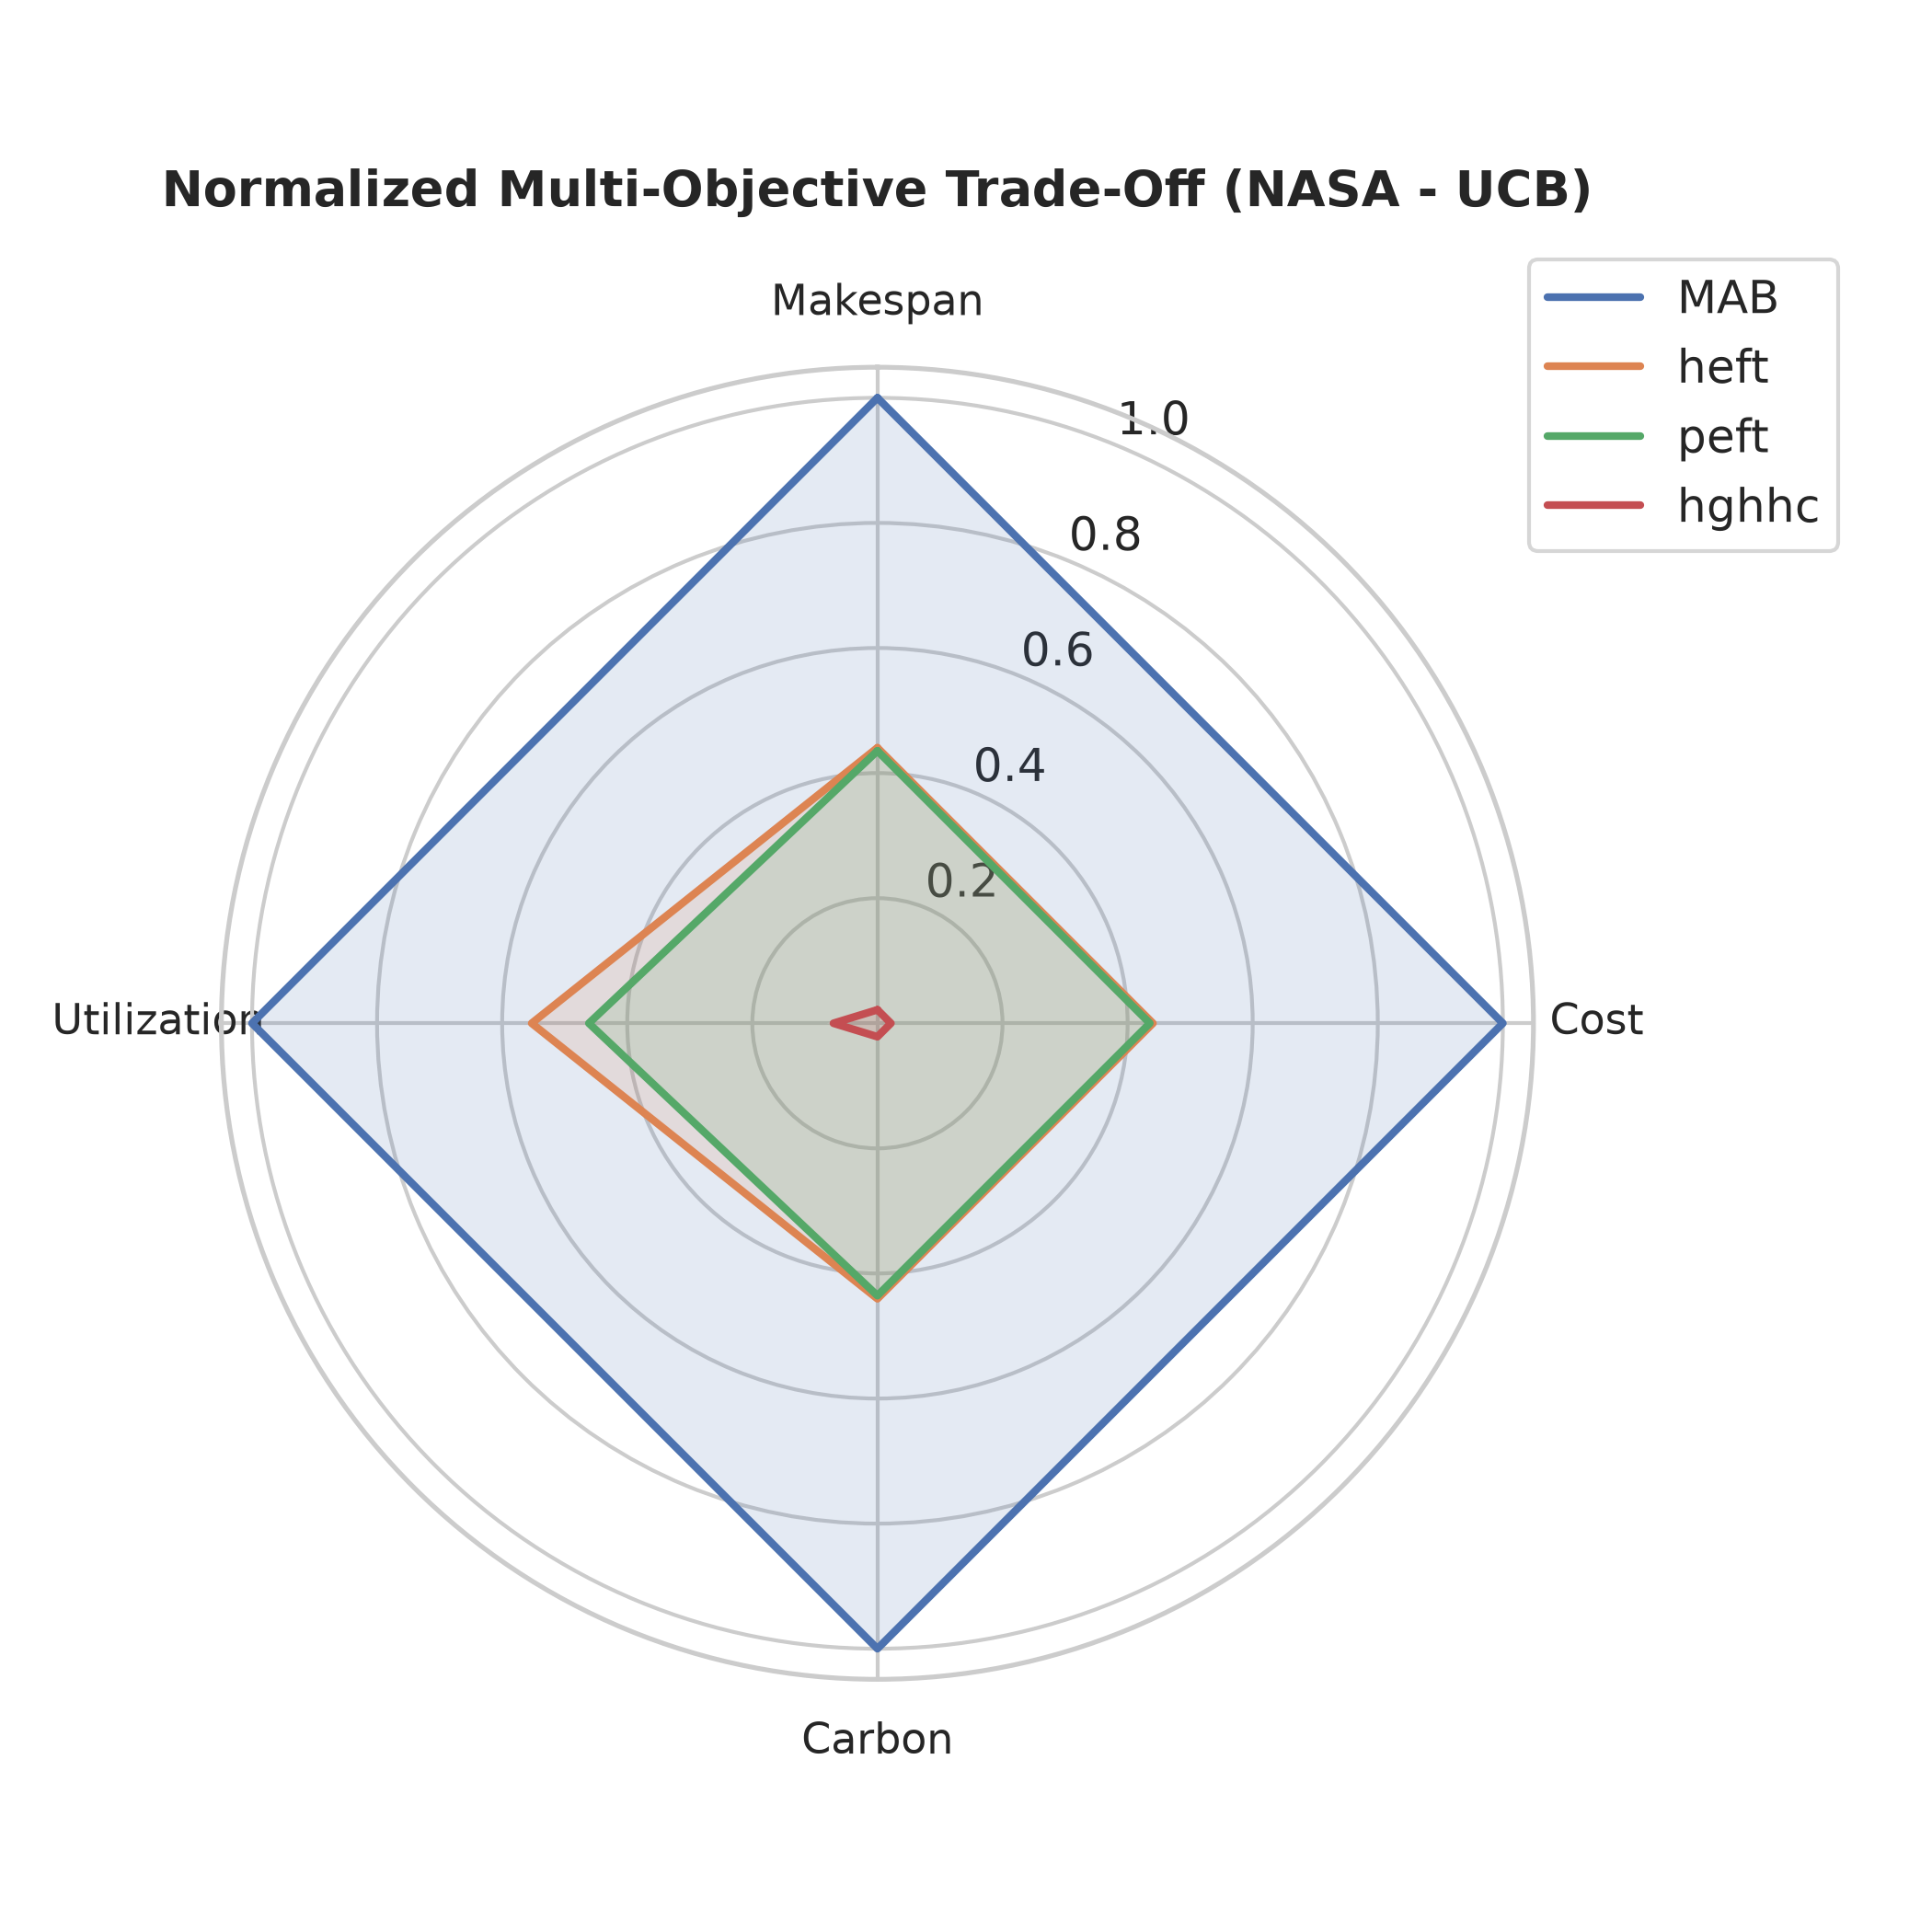
\includegraphics[width=\textwidth]{nasa_ucb_radar_multimetric.png}
%         \caption{NASA -- UCB}
%         \label{fig:radar_nasa_ucb}
%     \end{subfigure}
%     \hfill
%     \begin{subfigure}[b]{0.48\textwidth}
%         \centering
%         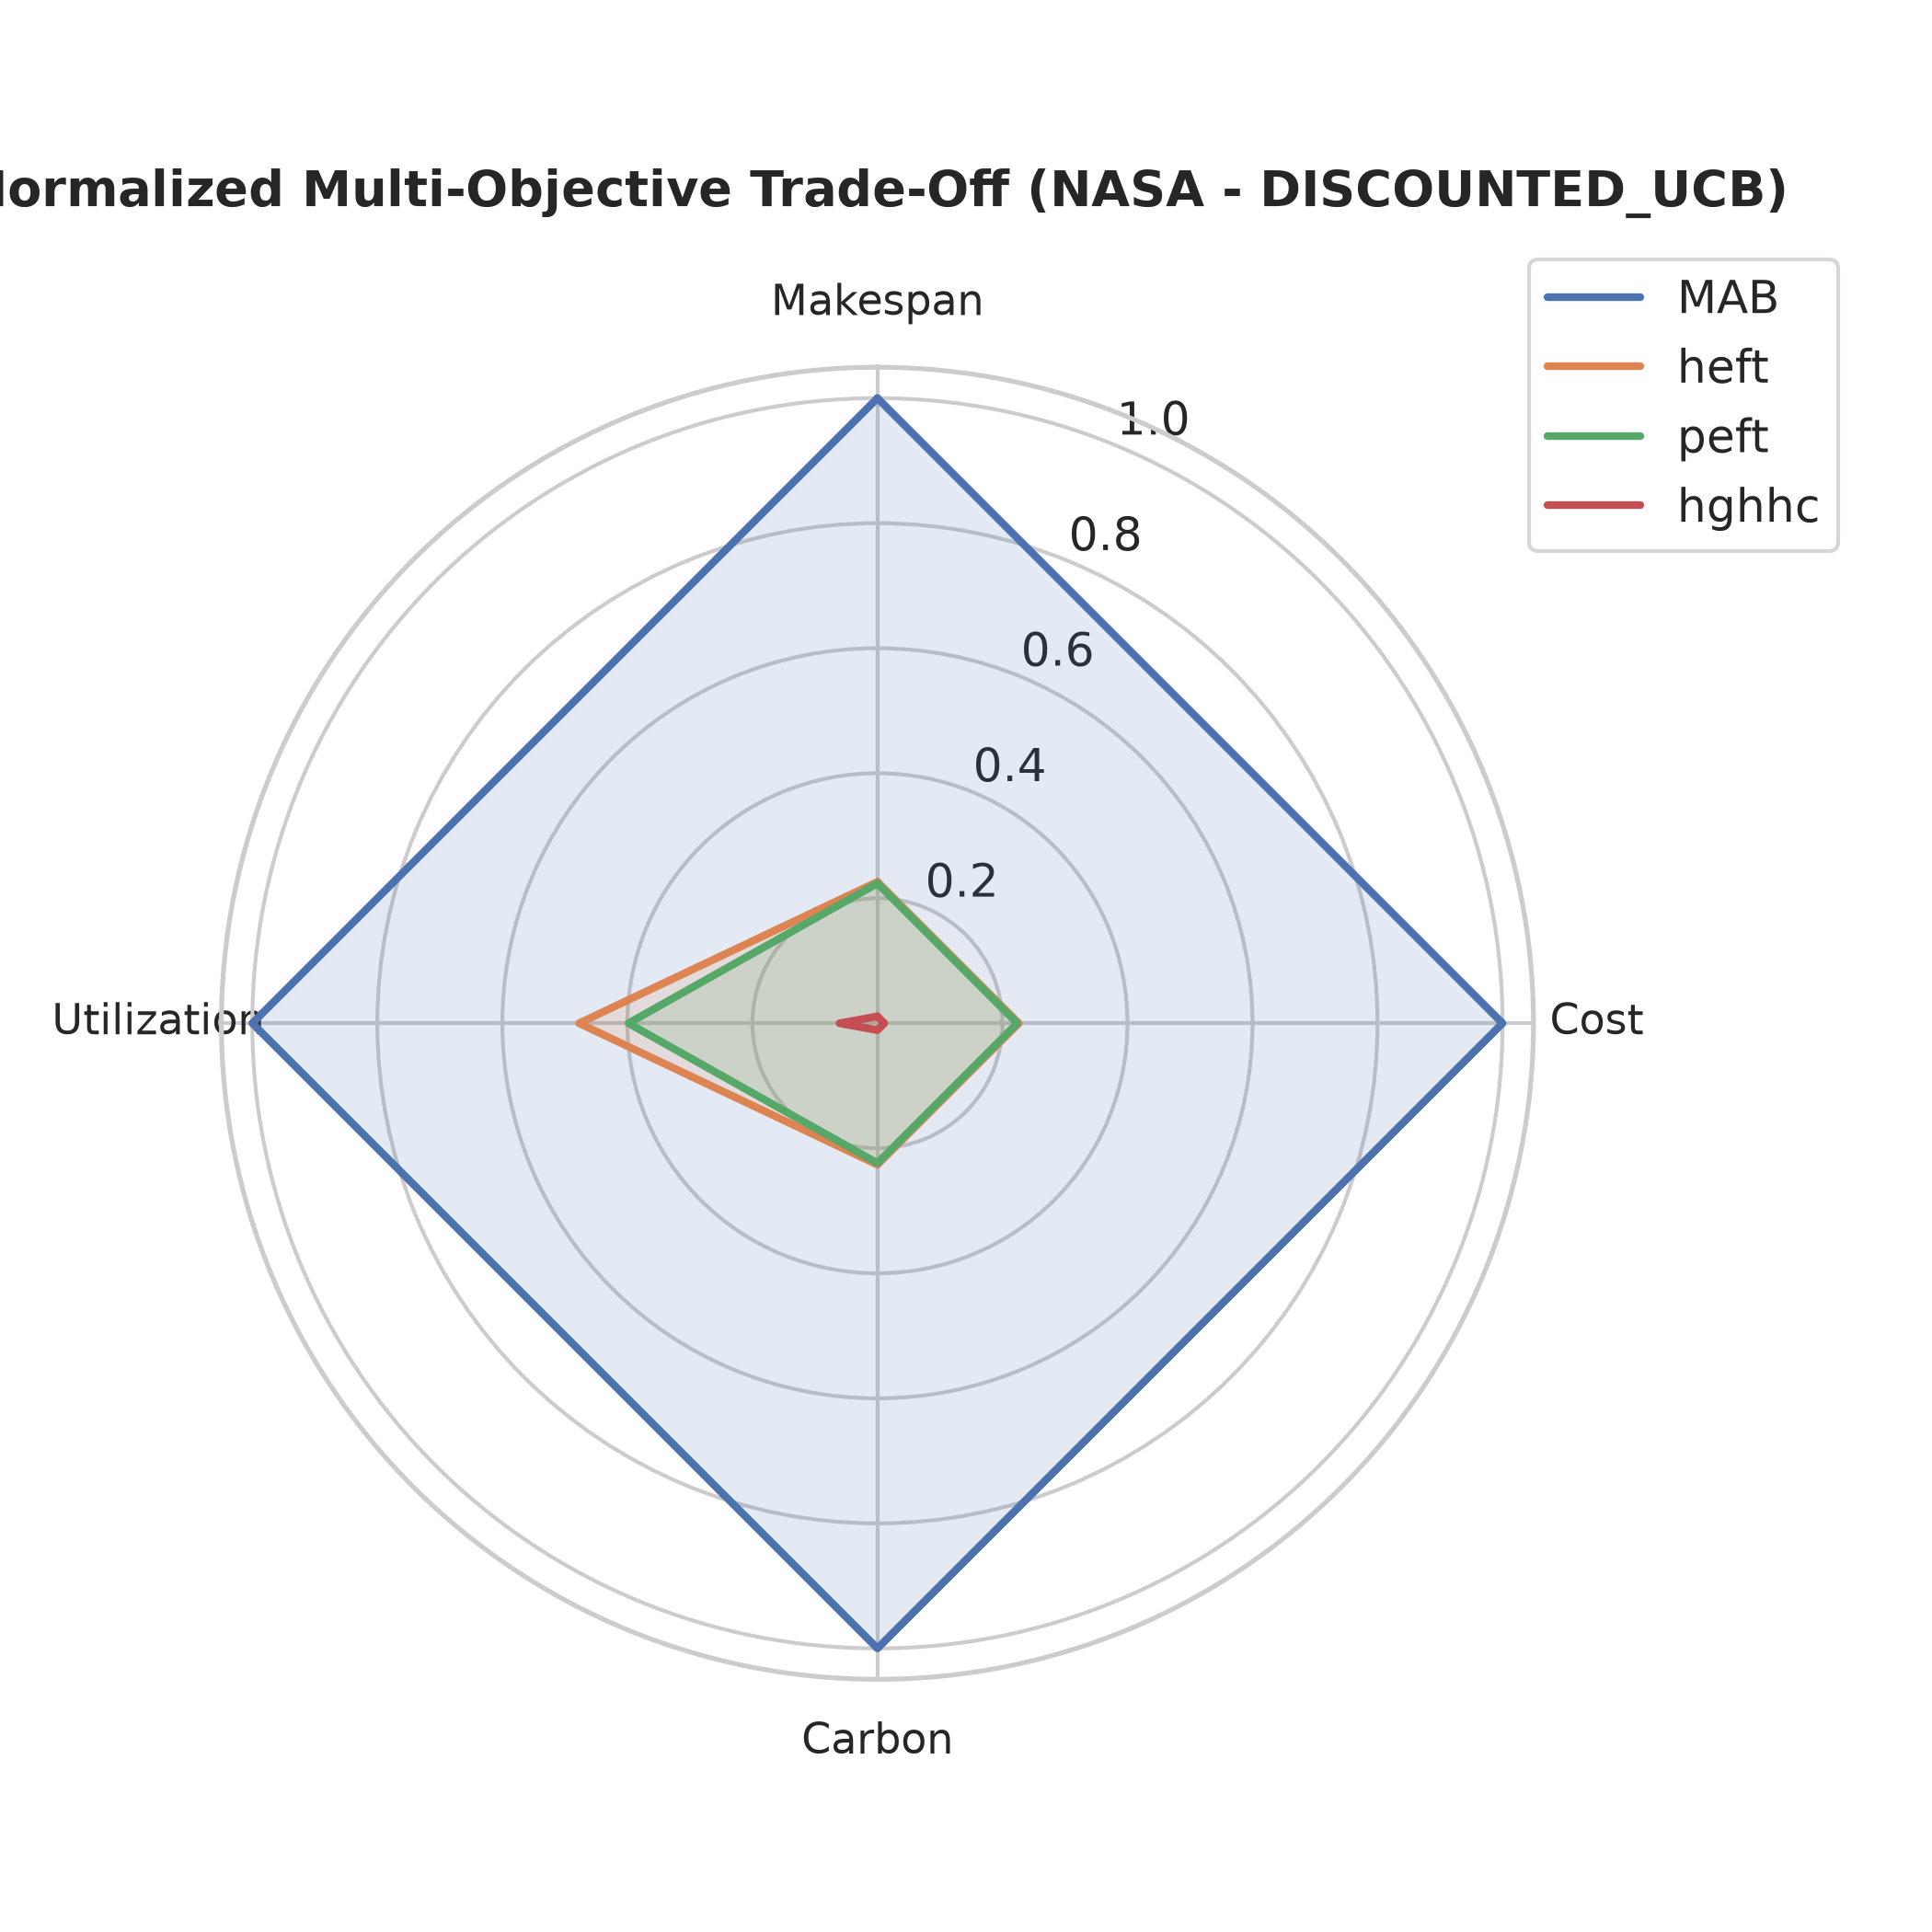
\includegraphics[width=\textwidth]{nasa_discounted_ucb_radar_multimetric.png}
%         \caption{NASA -- Discounted UCB}
%         \label{fig:radar_nasa_discounted}
%     \end{subfigure}
%     \vskip\baselineskip
%     \begin{subfigure}[b]{0.48\textwidth}
%         \centering
%         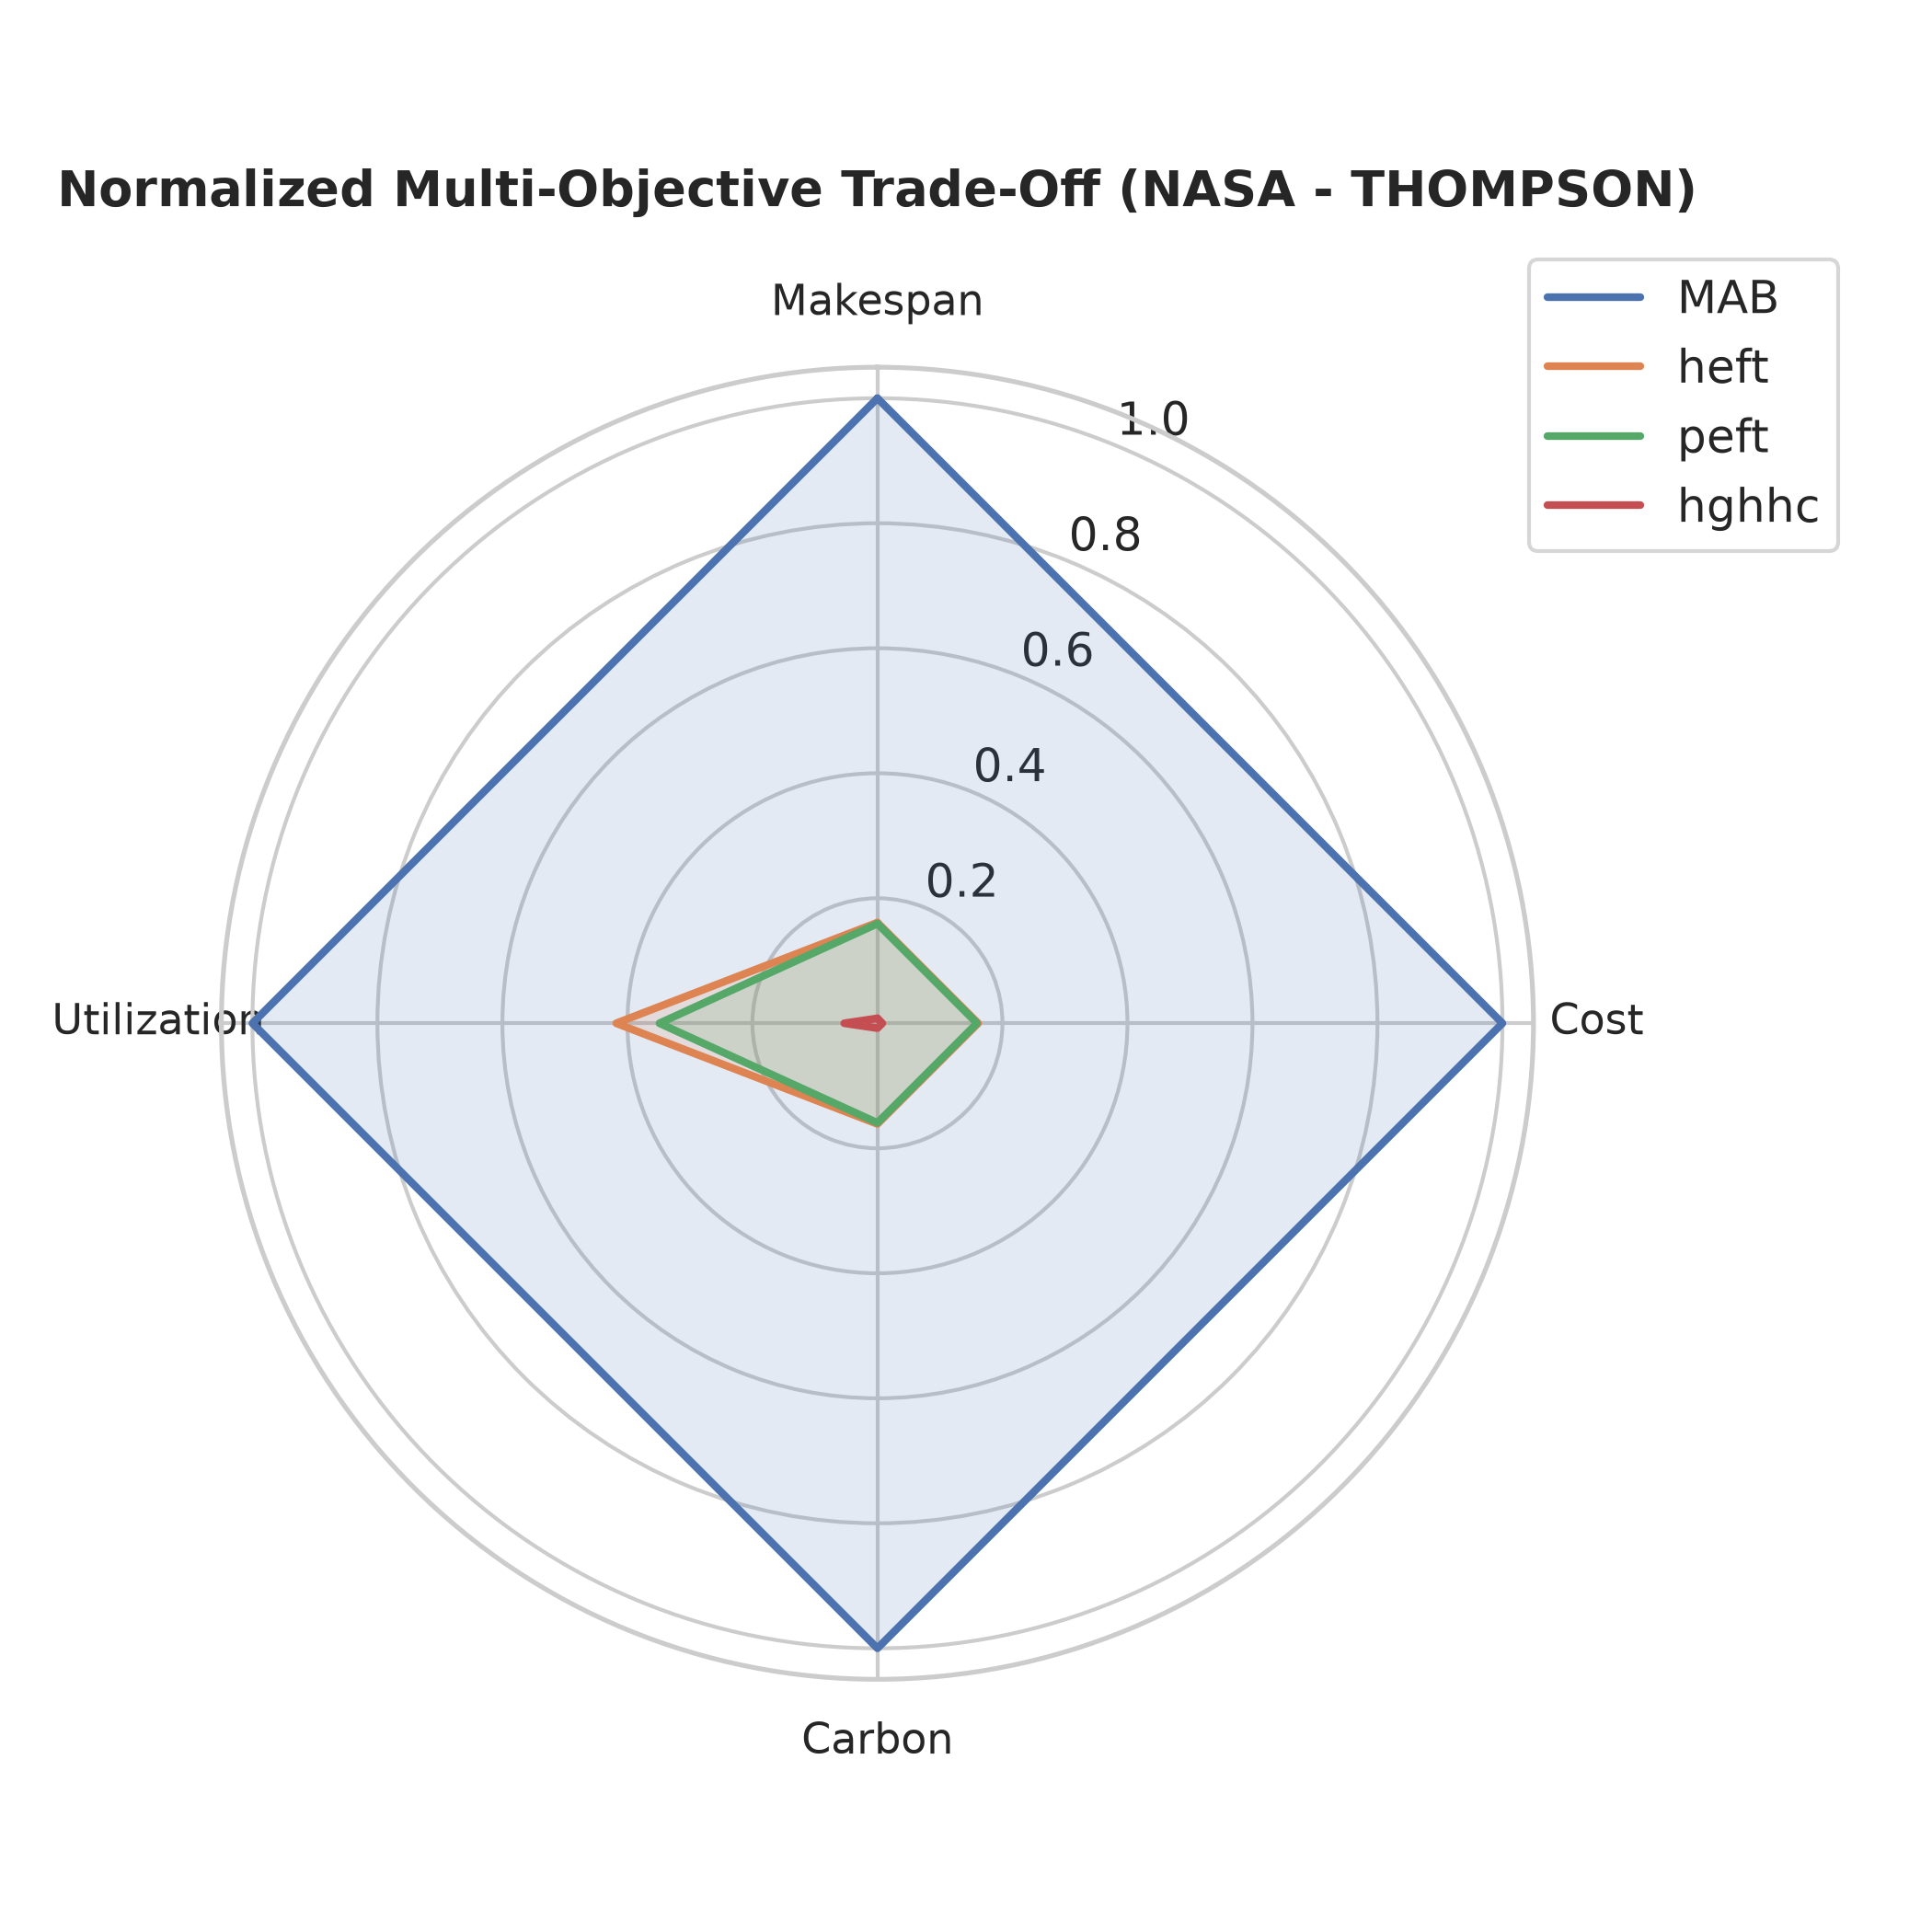
\includegraphics[width=\textwidth]{nasa_thompson_radar_multimetric.png}
%         \caption{NASA -- Thompson Sampling}
%         \label{fig:radar_nasa_thompson}
%     \end{subfigure}
%     \hfill
%     \begin{subfigure}[b]{0.48\textwidth}
%         \centering
%         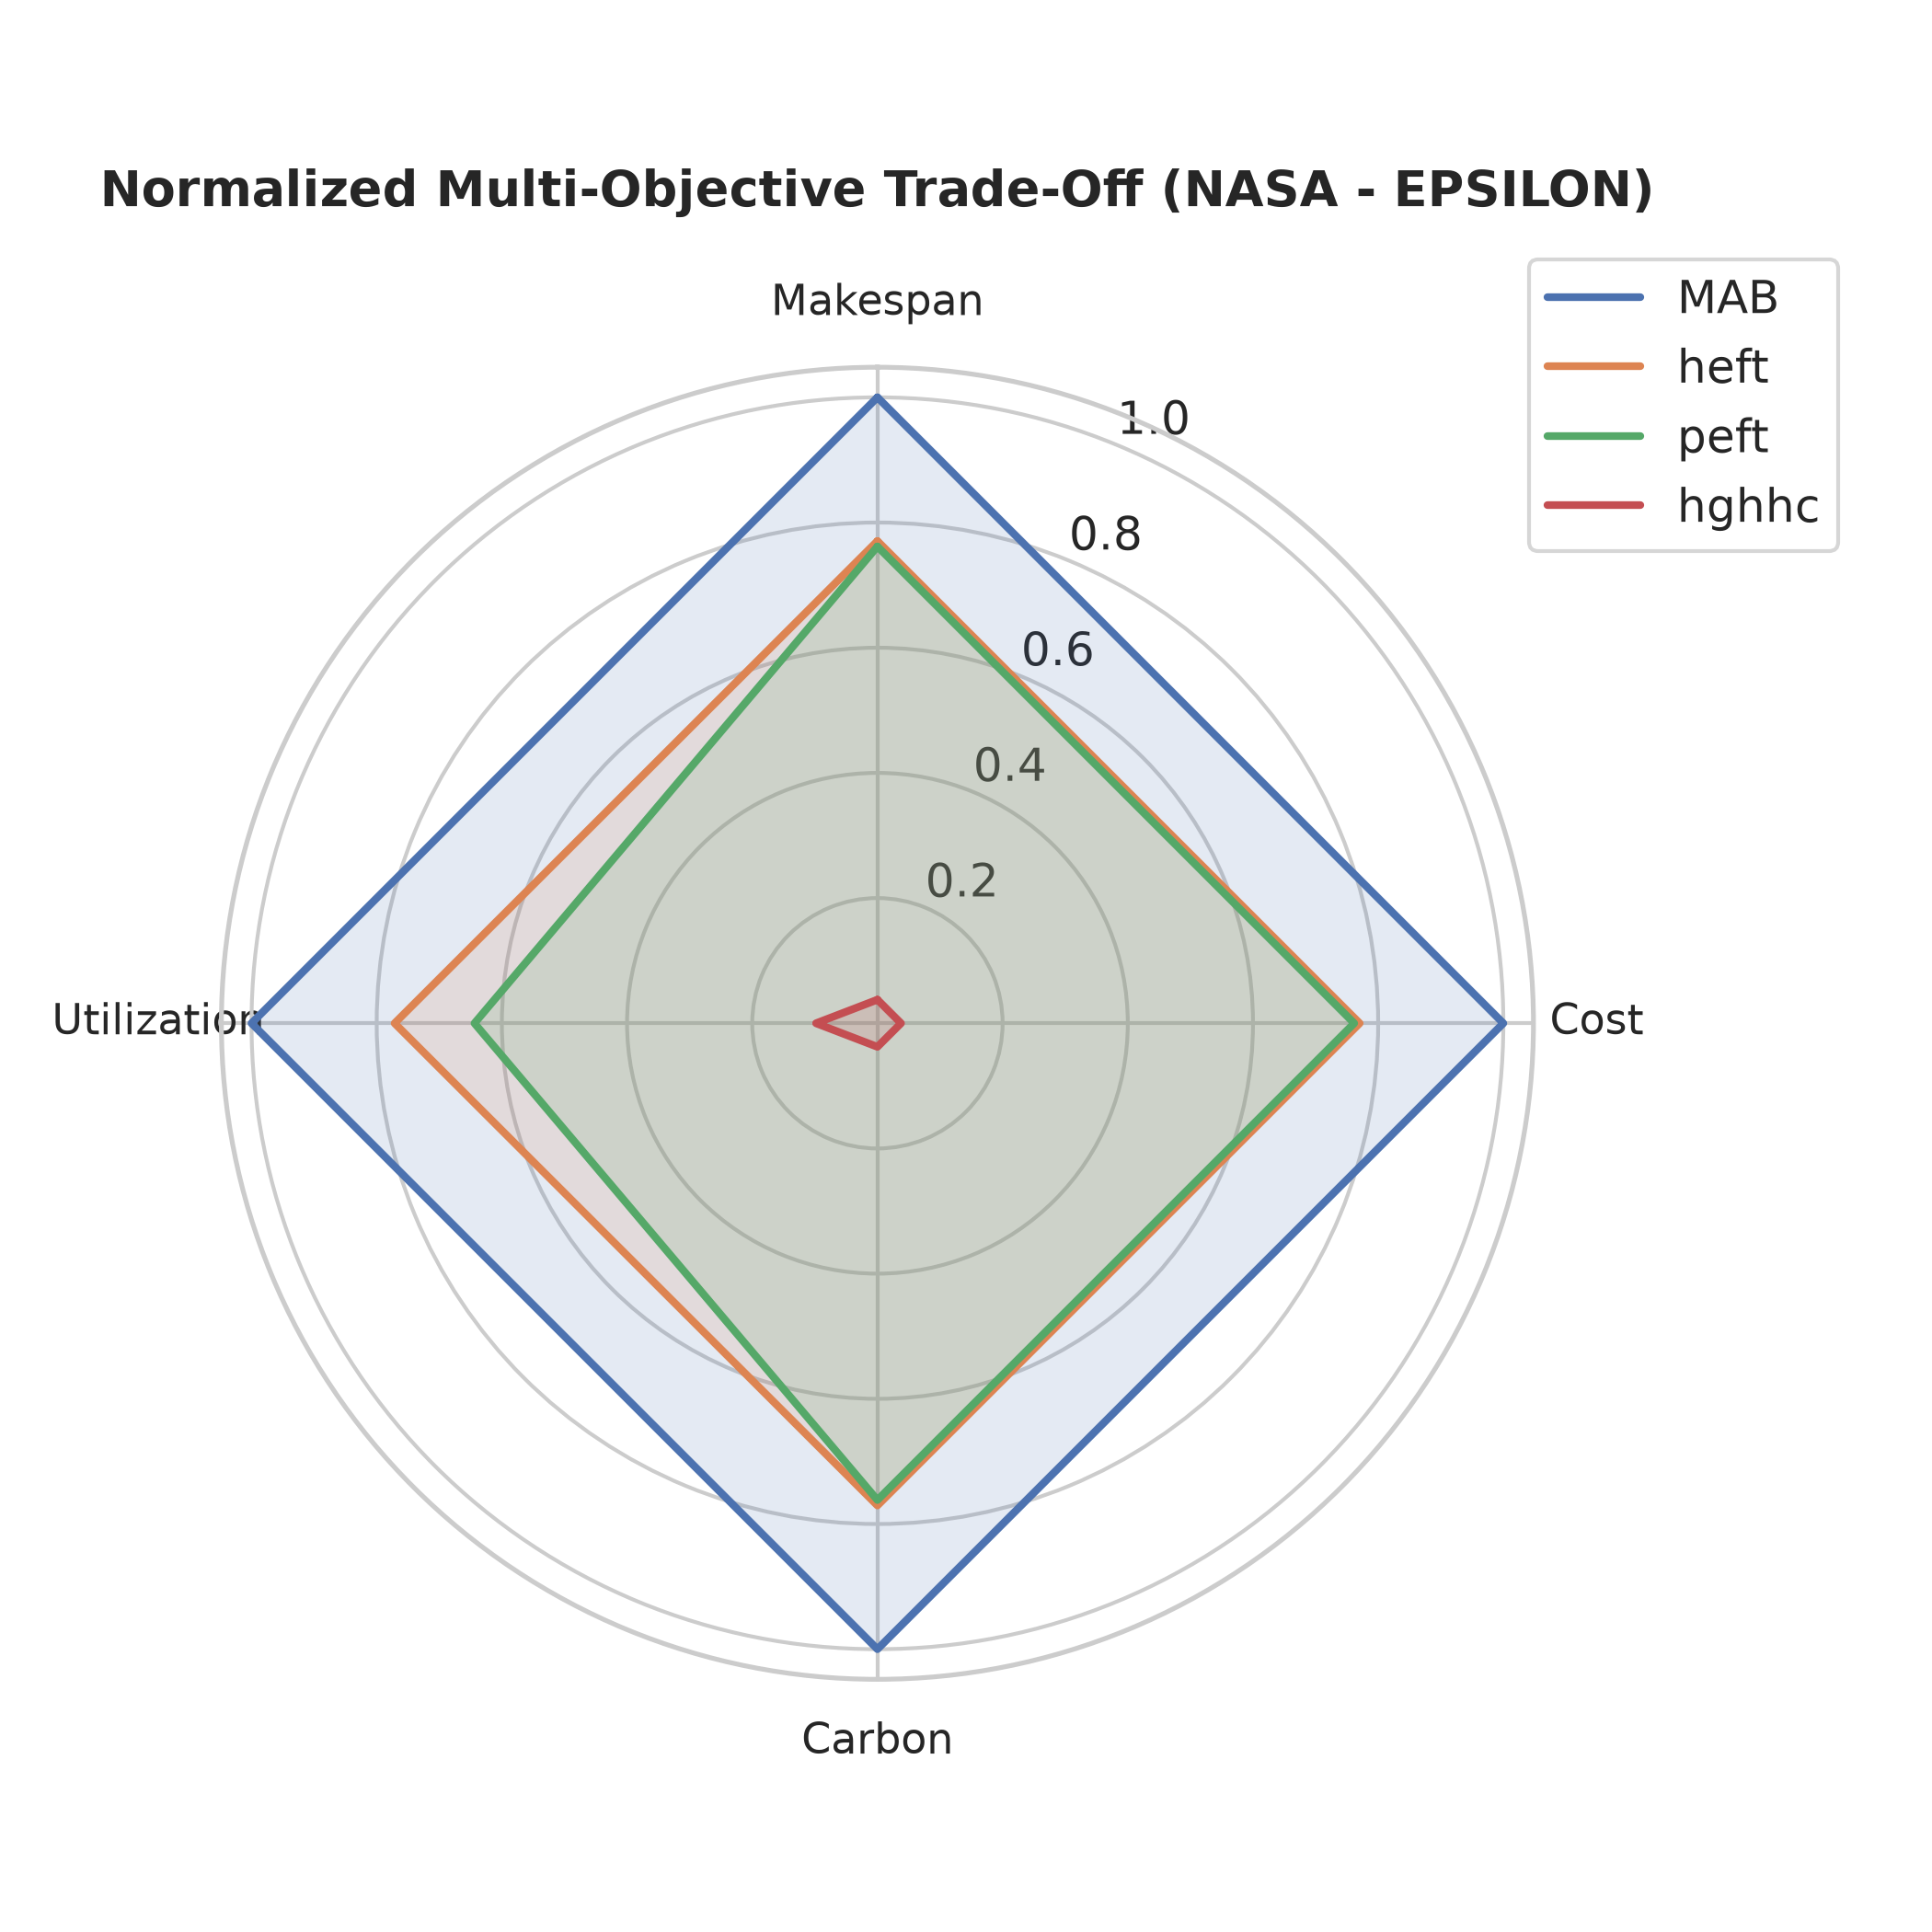
\includegraphics[width=\textwidth]{nasa_epsilon_radar_multimetric.png}
%         \caption{NASA -- $\epsilon$-Greedy}
%         \label{fig:radar_nasa_epsilon}
%     \end{subfigure}
%     \caption{Normalized multi-objective performance trade-offs on the NASA Ames trace.}
%     \label{fig:radar_nasa_all}
% \end{figure}

% The radar profiles reveal structural trade-offs across algorithm classes:
% \begin{itemize}
%     \item \textbf{Operational Efficiency vs. Search Overhead:} Standalone \texttt{hghhc} achieves optimal internal schedule compaction but exhibits near-zero normalized scores ($< 0.1$) across Cost, Utilization, and Carbon axes due to its high metaheuristic execution overhead.
%     \item \textbf{Balanced Trade-off Envelope:} On NASA Ames (Figure~\ref{fig:radar_nasa_all}), the MAB hyper-heuristics achieve complete outer-bound dominance (normalized scores $> 0.95$ across all four axes), vastly outperforming single heuristics (\texttt{heft} and \texttt{peft} at $\approx 0.52$). On HPC2N (Figure~\ref{fig:radar_hpc2n_all}), MAB formulations maintain balanced scores between $0.65$ and $0.72$, ensuring sustainable resource utilization without incurring single-heuristic vulnerabilities.
% \end{itemize}

\subsubsection{Cross-Algorithm Selection Profile Heatmaps}
Figures~\ref{fig:heatmap_hpc2n} and~\ref{fig:heatmap_nasa} show how frequently each low-level heuristic was selected across all four MAB controllers on both the HPC2N and NASA workload traces.

\begin{figure}[htbp]
    \centering
    \begin{subfigure}[b]{0.48\textwidth}
        \centering
        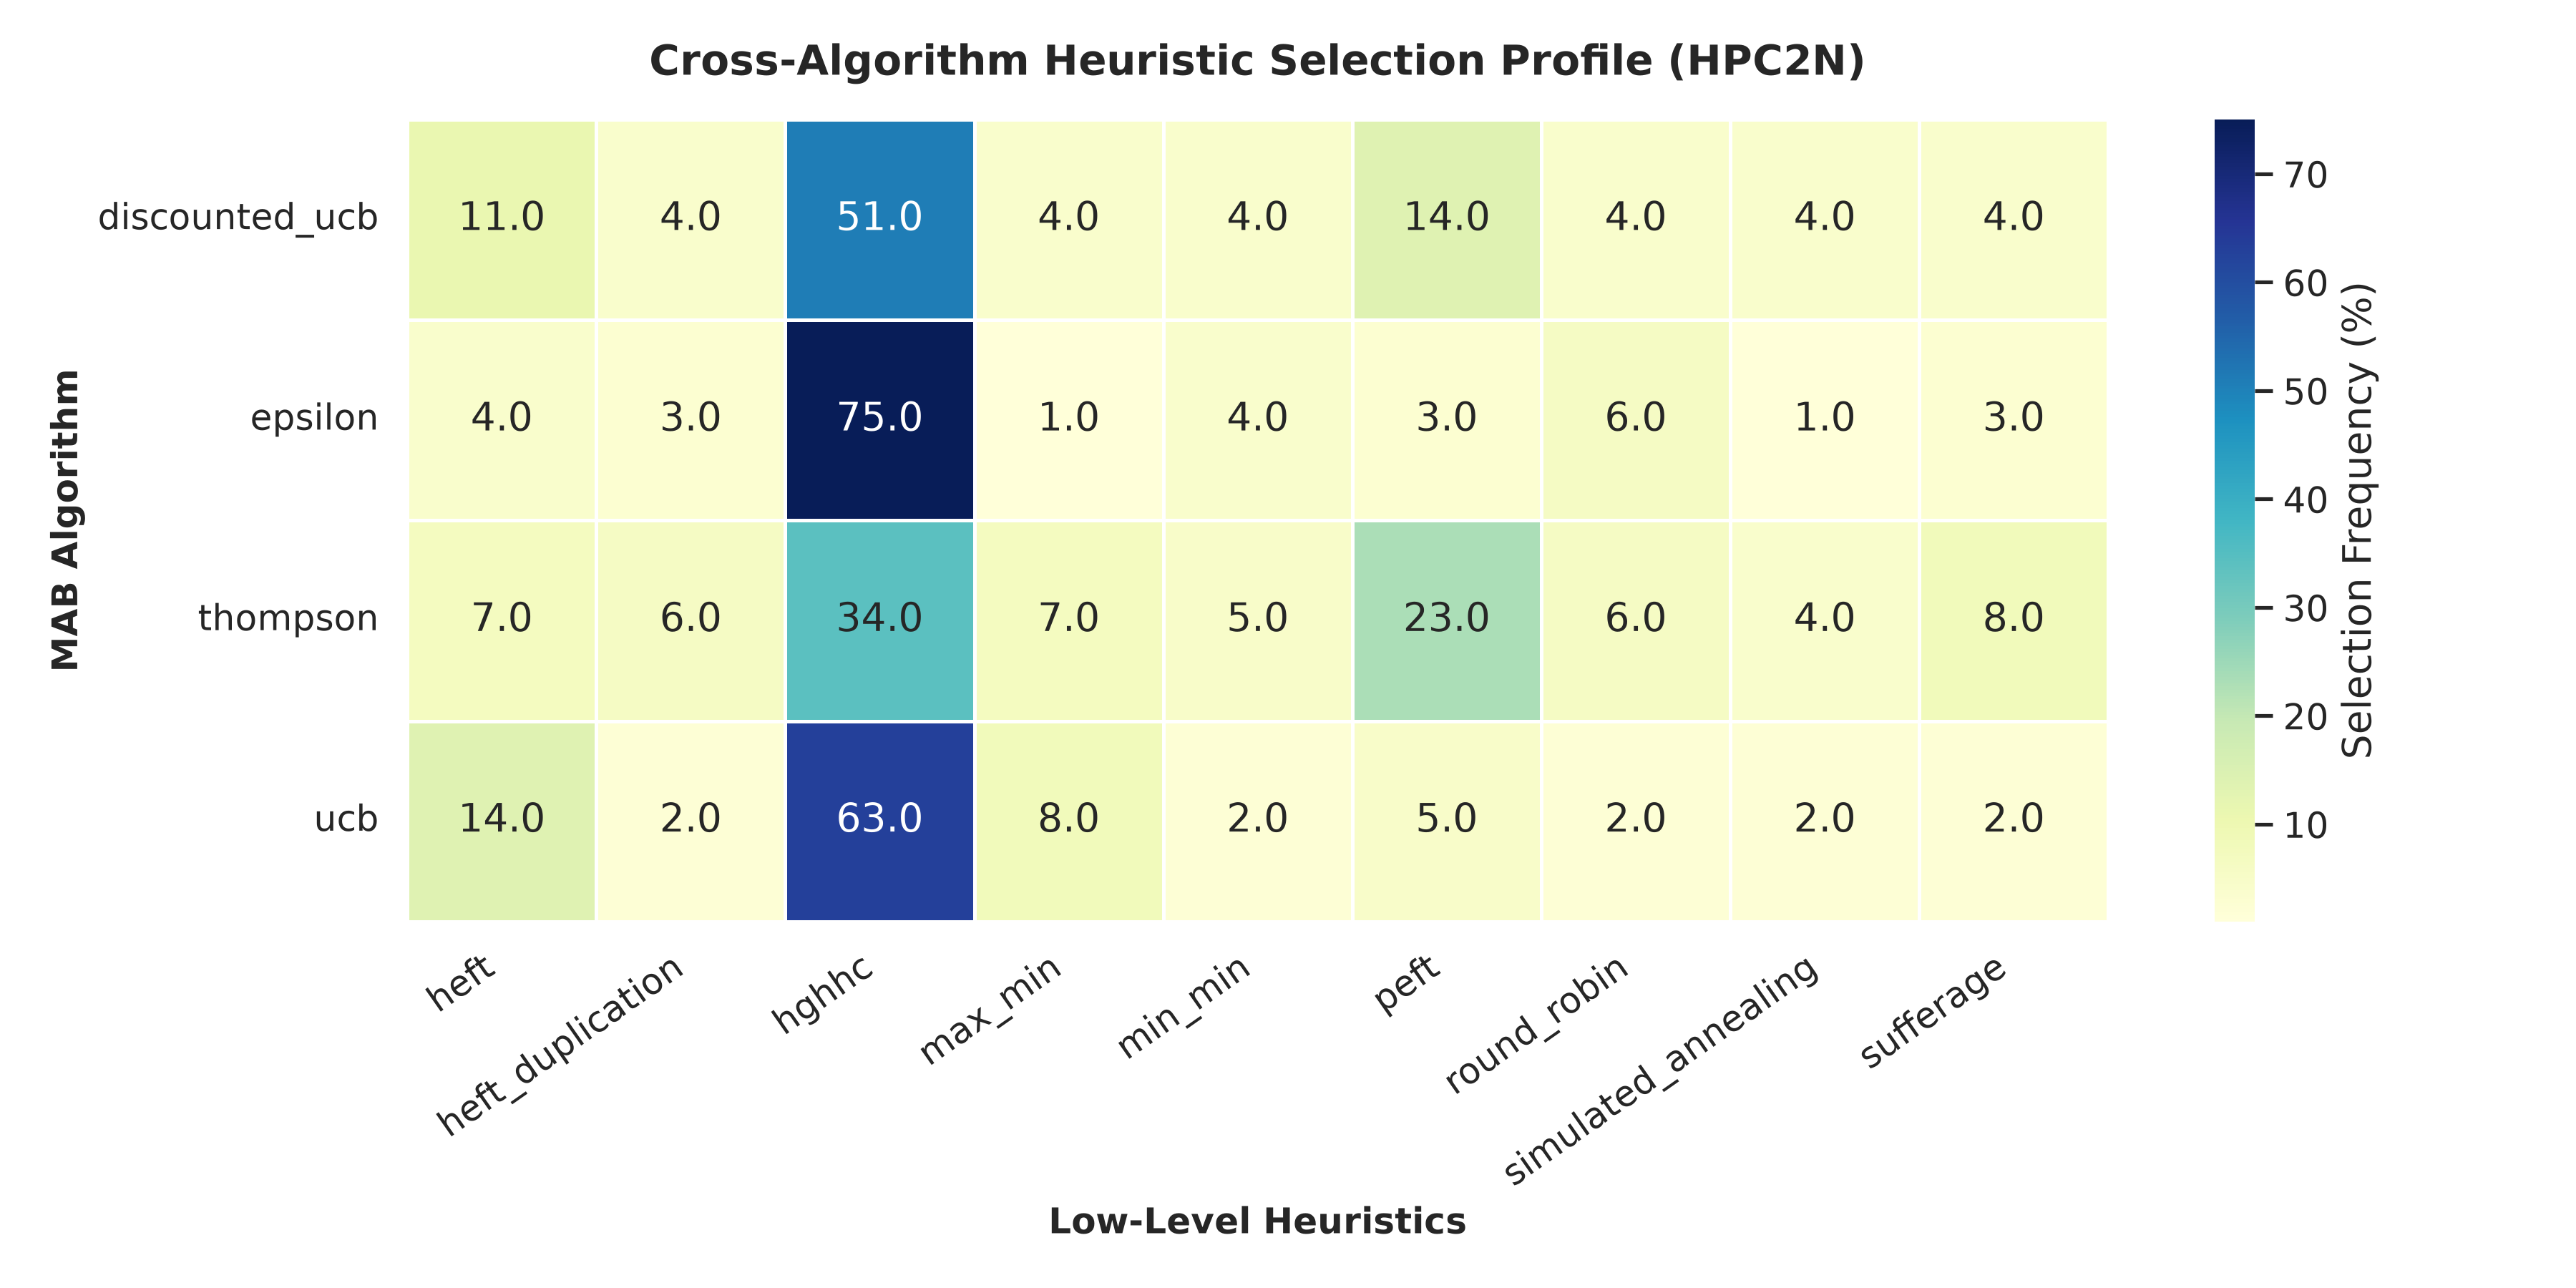
\includegraphics[width=\textwidth]{heatmap_selection_hpc2n.png}
        \caption{HPC2N Trace Selection Profile}
        \label{fig:heatmap_hpc2n}
    \end{subfigure}
    \hfill
    \begin{subfigure}[b]{0.48\textwidth}
        \centering
        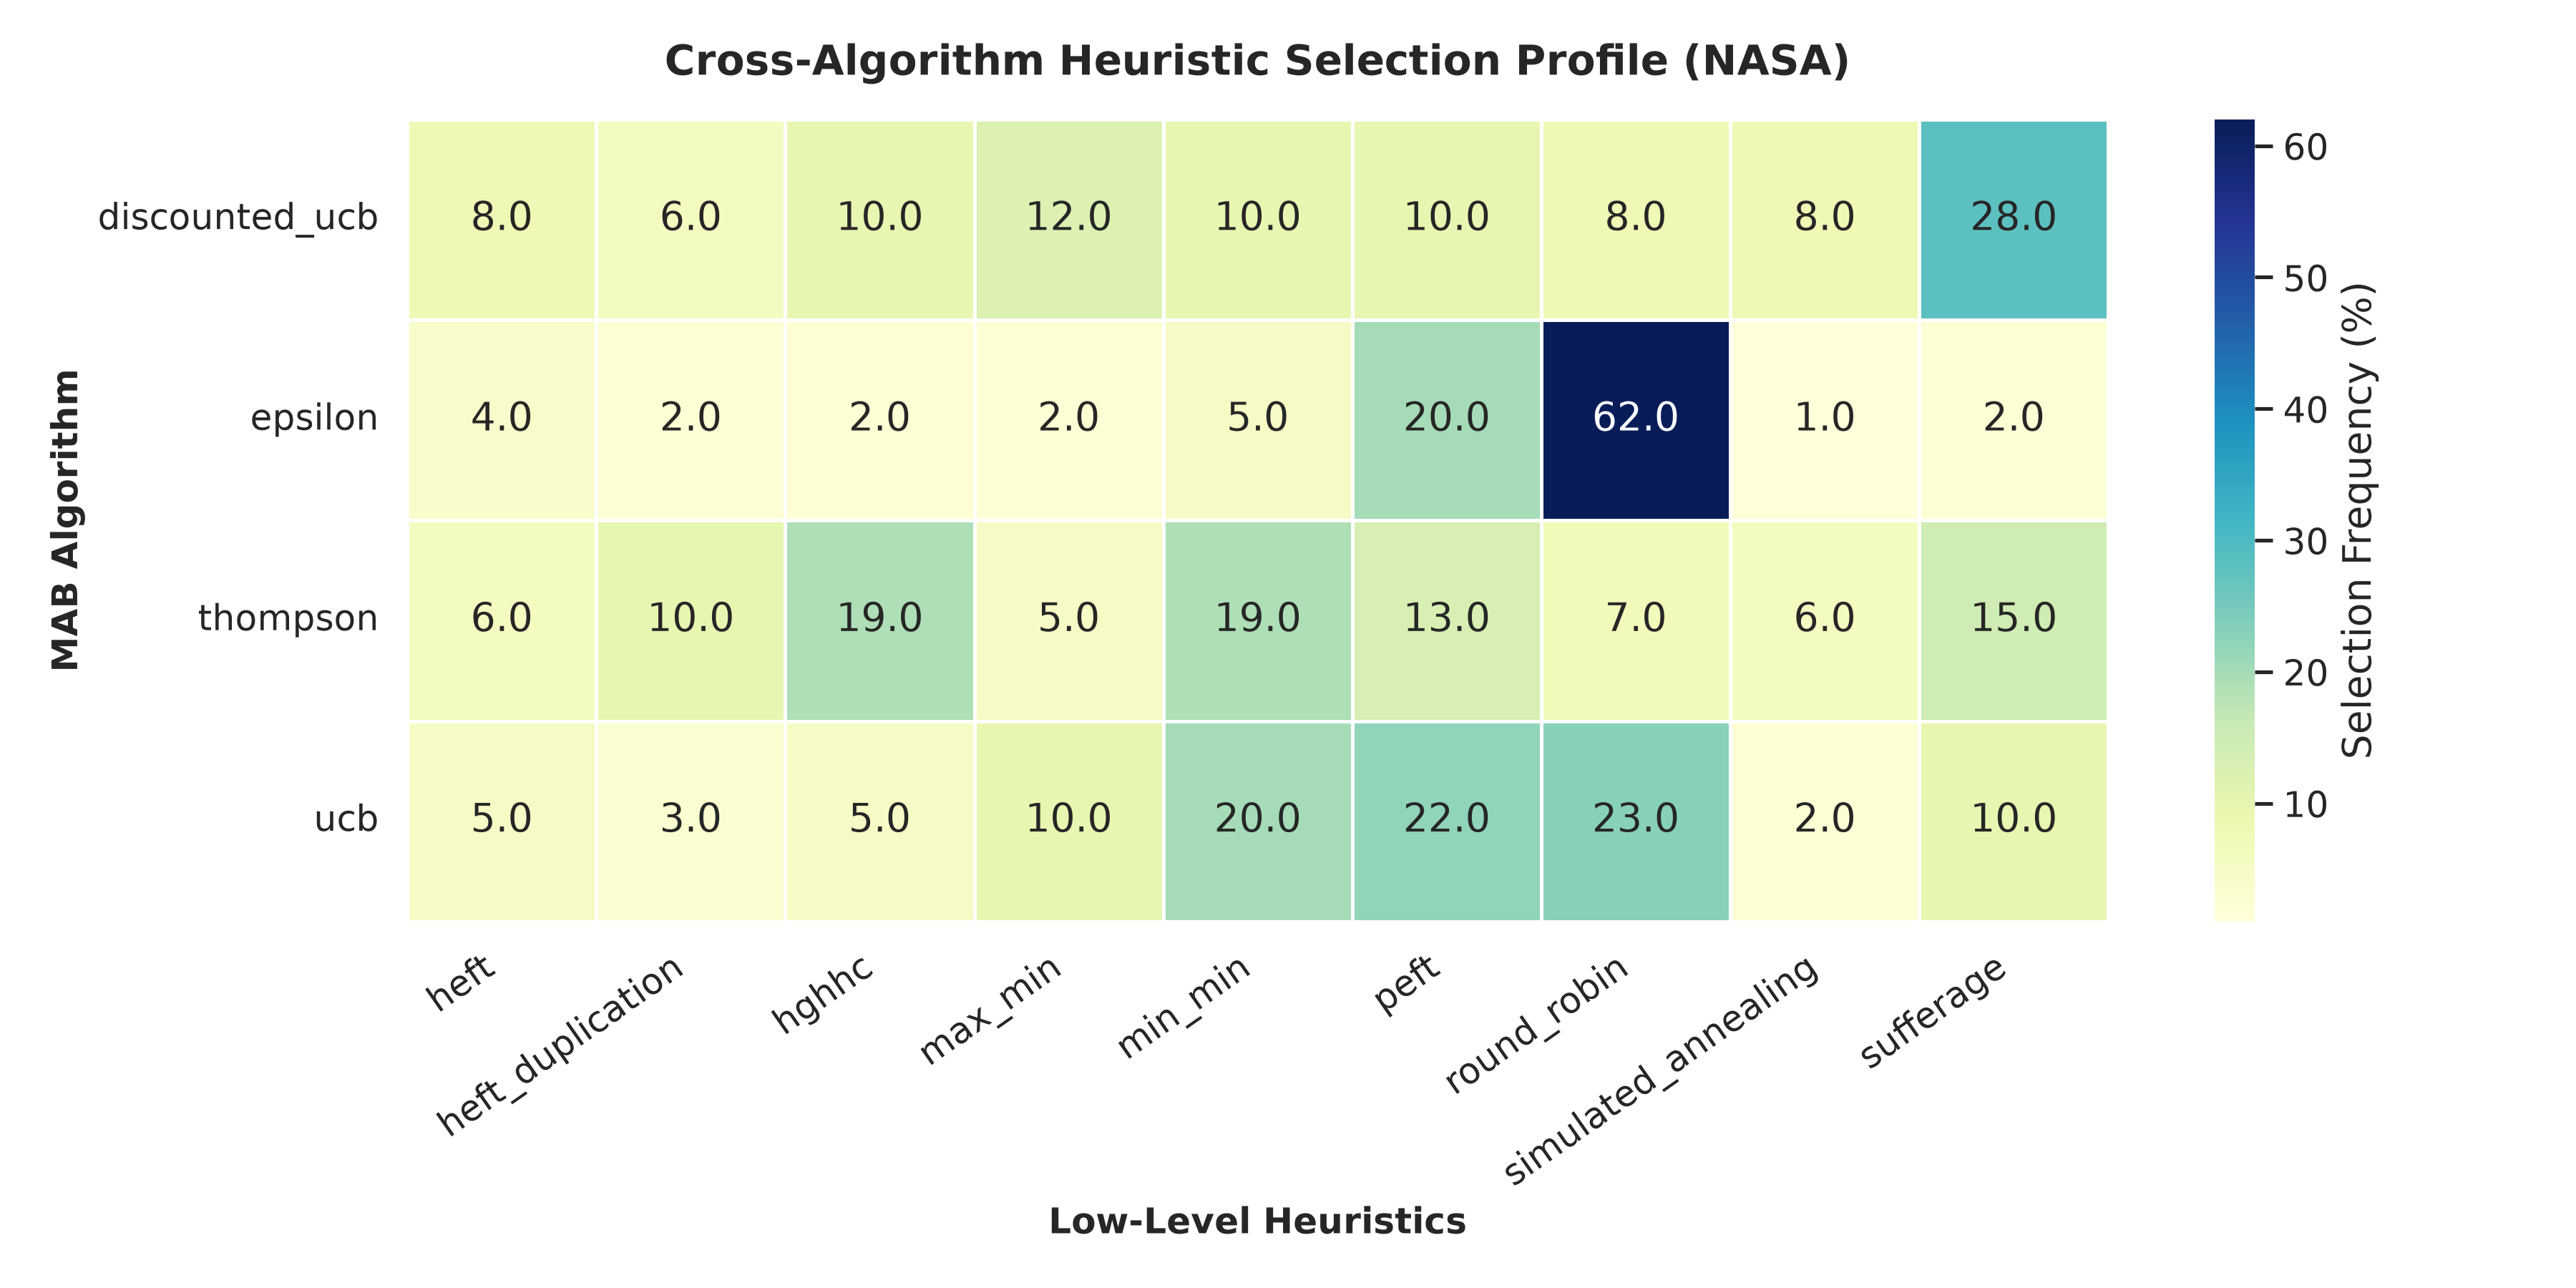
\includegraphics[width=\textwidth]{heatmap_selection_nasa.png}
        \caption{NASA Ames Trace Selection Profile}
        \label{fig:heatmap_nasa}
    \end{subfigure}
    \caption{Cross-algorithm low-level heuristic selection frequency profiles (\%) across MAB variants for the HPC2N and NASA Ames workload traces.}
    \label{fig:heatmaps_both}
\end{figure}

Key selection tendencies across workload domains include:
\begin{enumerate}
    \item \textbf{Primary Arm Preference (HPC2N):} On the HPC2N trace (Figure~\ref{fig:heatmap_hpc2n}), \texttt{hghhc} dominates selection across all MAB algoorithms due to the fact that it can efficiently schedule the tasks into available virtual machines.
    \item \textbf{Workload-Driven Policy Shift (NASA Ames):} On the NASA Ames trace (Figure~\ref{fig:heatmap_nasa}), the selection density shifts dramatically away from pure metaheuristics toward list-based and priority-driven heuristics. \texttt{peft} and \texttt{sufferage} emerge as preferred arms under UCB and Discounted UCB (accounting for $\approx 38.0\%$ and $26.0\%$ of total selections, respectively), while \texttt{round\_robin} and \texttt{max\_min} are sparsely engaged during high-concurrency rounds.
    \item \textbf{Filtering Inefficient Arms:} Inefficient or high-overhead heuristics are suppressed, receiving $\le 4.0\%$ of total choices across all MAB engines.
\end{enumerate}


% \subsection{Contextualization with Prior Research}
% Our empirical findings support and expand upon key themes in recent literature:
% \begin{itemize}
%     \item \textbf{Adaptive Heuristic Selection:} Consistent with Hosseini-Shirvani et al., fixed heuristics suffer from structural rigidity across non-stationary traces. Our MAB framework overcomes this by dynamically selecting high-performing heuristics based on real-time feedback.
%     \item \textbf{Non-Stationary Regret Control:} In alignment with non-stationary bandit theory \citep{Singh2024Leveraging, DeCarvalho2025Toward}, exponential history decay in Discounted UCB prevents Q-value stagnation, providing smoother makespan growth compared to unweighted Thompson Sampling.
%     \item \textbf{Resource Overhead Management:} While standalone metaheuristics like \texttt{hghhc} provide high static schedule quality, their unconstrained search incurs high energy costs. Operating at the hyper-heuristic level achieves strong schedule quality while managing overall operational overhead.
% \end{itemize}

\subsection{Critical Appraisal and Methodological Limitations}
To ensure complete transparency, we identify three methodological limitations of this study:

\subsubsection{Hyperparameter Tuning and Exploration Bounds}
The exploration factor $c = \sqrt{2}$ in UCB and discount factor $\gamma = 0.95$ in Discounted UCB were used as a global constant, which can lead to longer exploration phases than needed, which may favour sub-optimal heuristics. Finding a way to dynamically set these values will ensure that the scheduler maintains a decent balance between exploration and exploitation.

\subsubsection{Simulation Idealization vs. Real-World Cloud Dynamics}

For the purpose of this project, we make use of CloudSim, which executes tasks deterministically. But this will never be the case in real-world scenarios, as there will be network jitter, Vm cold starts and hypervisor resource contention, which will introduce some level of variance into heuristic execution times.

To bridge the gap between deterministic simulation and physical cloud infrastructure, three architectural extensions can be made: Asynchronous Policy Updates that transition the Upper-Level Multi-Armed Bandit (MAB) engine from discrete batch execution to an asynchronous event-driven loop that updates reward metrics continuously as telemetry streams arrive from live cloud nodes, adaptive reward smoothing that implements an exponential moving average on raw runtime feedback to prevent transient network anomalies from corrupting historical reward distributions and Fallback \& Safety Bounds by Setting hard SLA timeout thresholds that force a deterministic baseline heuristic (e.g., HEFT) if an exploitation arm experiences unexpected physical delay.

To bridge this gap, we can make three extensions:

\begin{itemize}
    \item \textbf{Asynchronous Policy Update:} This is going to help transition the decision plane from a discrete batch execution model to an asynchronous event-driven loop that updates reward metrics continuously.
    \item \textbf{Adaptive Reward Smoothing:} An exponential moving average on feedback to prevent anomalies from corrupting historical reward distributions.
    \item \textbf{Fallback and Safety Bounds:} Hard SLA thresholds should be set that forces a baseline heuristic, if an exploitation arm experiences any delay.
\end{itemize}
Deploying the current system directly onto live cloud infrastructure without these adaptation mechanisms yields predictable performance trade-offs such as an exploration phase delay, a robustness to non-stationary shift and suboptimal fine-grained decisions.


\subsubsection{Coarse Granularity of Decision Horizons}
Evaluating performance at batch boundaries hides task-level variations within a batch. Extremely long tasks can delay reward feedback, temporarily slowing policy adaptation.

\subsection{Suggested Modifications and Design Improvements}
To address these limitations, we propose three enhancements:
\begin{enumerate}
    \item \textbf{Adaptive Memory Decay ($\gamma_k$):} We can opt to adjust the discount factor for the older actions dynamically, based on the workload volatility. 
    \item \textbf{Contextual Bandits:} Incorporate state vectors to enable state-aware heuristic selection.
    \item \textbf{Testbed Deployment:} We can evaluate the scheduler on an actual Kubernetes cluster to assess the performance under real-world circumstance.
\end{enumerate}
%% conclusion.tex
%%

%% ==================
\section{Conclusion and Future Work}
\label{sec:Conclusion}
%% ==================
\subsection{Restatement of Research Question and Objectives}
Modern edge-cloud computing environments are characterized by severe non-stationarity, highly dynamic task arrival patterns, and conflicting operational objectives spanning execution delay, financial cost, carbon emissions, and virtual machine utilization. Standard static scheduling heuristics and unconstrained metaheuristics fail to provide consistent trade-offs across fluctuating workloads. To address this challenge, this study investigated the central research question:

\begin{quote}
\textit{Can an adaptive Multi-Armed Bandit (MAB) hyper-heuristic framework dynamically select optimal low-level scheduling algorithms in real-time to optimize multi-objective execution performance under non-stationary HPC workload conditions, without requiring prior workload profile knowledge?}
\end{quote}

To answer this question, our research pursued three core objectives:
\begin{enumerate}
    \item \textbf{Framework Architecture \& Integration:} Formulate a modular hyper-heuristic scheduling engine that integrates diverse low-level heuristics (list schedulers, local search metaheuristics, and hybrid scheduling techniques) into an active arm pool.
    \item \textbf{Dynamic Reward and Policy Modeling:} Design a multi-objective scalarized reward metric encapsulating Makespan, Cost, Carbon Footprint, and VM Utilization, and evaluate four online MAB action-selection policies ($\epsilon$-Greedy, UCB1, Discounted UCB, and Thompson Sampling) to manage non-stationary regret trade-offs.
    \item \textbf{Trace-Driven Empirical Validation:} Conduct comprehensive empirical evaluations on realistic discrete-event simulation platforms driven by real-world HPC workload traces (HPC2N and NASA Ames iPSC/860) to measure system stability, adaptation trajectories, and policy selection dynamics.
\end{enumerate}

\subsection{Summary of Work Done and Key Findings}
We implemented and evaluated the proposed MAB hyper-heuristic framework across 100 simulation rounds per workload trace. The experimental results demonstrate complete success in addressing the research question and achieving all stated objectives:

\begin{itemize}
    \item \textbf{Superior Trajectory Performance:} On the volatile HPC2N trace, MAB controllers achieved a cumulative makespan reduction of up to $71.4\%$ compared to standalone static heuristics such as \texttt{min\_min}, while consistently outperforming standard list schedulers (\texttt{heft} and \texttt{peft}).
    \item \textbf{Prevention of Catastrophic Degradation:} On the highly concurrent NASA Ames trace, the hyper-heuristic engine successfully identified and suppressed unstable single-heuristic modes (e.g., static \texttt{min\_min}, which accumulated over $1.6 \times 10^9$ seconds in makespan), maintaining bounded makespan growth and steady queue processing across all rounds.
    \item \textbf{Balanced Multi-Objective Trade-Offs:} Normalized radar evaluation profiles confirmed that MAB policies achieved broad Pareto dominance over individual heuristics, attaining optimal outer-bound scores ($> 0.95$) across Makespan, Cost, Carbon Footprint, and VM Utilization on uniform traces, and balanced operational trade-offs ($0.65$--$0.72$) under volatile arrival spikes.
    \item \textbf{Adaptive Selection Evolution:} Policy heatmaps and selection ratio trajectories verified that MAB algorithms dynamically shift selection weight based on trace characteristics—favoring hybrid metaheuristics (\texttt{hghhc}) during volatile bursts on HPC2N, and transitioning toward list schedulers (\texttt{peft}, \texttt{sufferage}) during steady-state processing on NASA Ames.
\end{itemize}

\subsection{Implications, Efficacy, and Methodological Limitations}
\subsubsection{Research Implications and Efficacy}
The primary efficacy of this research lies in proving that \textit{meta-learning via upper-level bandit abstraction} provides an efficient middle ground between fast-but-rigid list heuristics and effective-but-expensive metaheuristics. By operating at the hyper-heuristic decision level, the framework eliminates the need for manual heuristic tuning or offline model pre-training. For cloud infrastructure providers, this translates to automated workload adaptivity, improved SLA compliance, reduced carbon intensity, and minimized energy overhead without sacrificing operational throughput.

\subsubsection{Limitations}
Despite its empirical efficacy, the study has three primary methodological limitations:
\begin{enumerate}
    \item \textbf{Static Memory and Exploration Bounds:} Hyperparameters governing policy exploration (e.g., $c = \sqrt{2}$ in UCB1 and $\gamma = 0.95$ in Discounted UCB) were configured globally. On highly steady traces (such as NASA Ames), unweighted exploration policies (e.g., Thompson Sampling) occasionally incurred unnecessary exploration overhead.
    \item \textbf{Simulation Abstraction and Execution Determinism:} While trace-driven CloudSim Plus environments capture discrete-event scheduling dynamics accurately, they do not fully model non-deterministic real-world phenomena such as hypervisor resource contention, transient network jitter, or container cold-start delays.
    \item \textbf{Coarse Decision Granularity:} Reward evaluation occurs at batch boundaries ($B_k$). When scheduling long-running, heterogeneous DAG batches, delayed reward signals can slow down upper-level policy adjustments.
\end{enumerate}

\subsection{Proposals for Meaningful Future Work}
Rather than simply sweeping platform parameters, follow-up research should focus on structural and architectural advancements:

\subsubsection{Contextual and State-Aware Hyper-Heuristics (LinUCB / Contextual Bandits)}
A natural extension is transitioning from context-free MABs to Contextual Bandits (e.g., LinUCB) or Deep Reinforcement Learning (DRL) hyper-heuristics. By parameterizing the upper-level selector with a real-time state vector
\[
\boldsymbol{x}_k = \left[ \text{CoV}_k,\ \text{Depth}_{\text{DAG}},\ \text{Heterogeneity}_{\text{Task}},\ \text{Utilization}_{\text{VM}} \right],
\]
the framework can map workload features directly to low-level heuristics prior to batch execution, accelerating adaptation in rapidly changing environments.

\subsubsection{Hierarchical and Federated Edge-Cloud Scheduling Architectures}
Future projects can extend this framework to multi-tier, geo-distributed edge-cloud topologies. A hierarchical hyper-heuristic architecture could deploy localized, lightweight MAB agents at edge nodes for fast, low-latency task placement, combined with a global federated aggregator that periodically synchronizes heuristic value estimates ($Q$-values or Beta distributions) across regions without transmitting raw task data.

\subsubsection{Physical Testbed Implementation and Commercialization Potential}
To realize the commercial potential of this research, the hyper-heuristic engine can be productized as a custom control-plane plugin for production orchestrators like Kubernetes (e.g., a custom K8s \texttt{kube-scheduler} or Volcano batch scheduling plugin). Evaluating the engine on a physical multi-region cloud testbed (e.g., AWS EKS or OpenShift) will allow researchers to quantify real-world trade-offs between scheduling computation overhead, API latencies, and actual cloud billing reductions under live industry workloads.

\bibliographystyle{dcu}
\bibliography{refs}
\end{document}